\documentclass[twoside]{book}

% Packages required by doxygen
\usepackage{fixltx2e}
\usepackage{calc}
\usepackage{doxygen}
\usepackage[export]{adjustbox} % also loads graphicx
\usepackage{graphicx}
\usepackage[utf8]{inputenc}
\usepackage{makeidx}
\usepackage{multicol}
\usepackage{multirow}
\PassOptionsToPackage{warn}{textcomp}
\usepackage{textcomp}
\usepackage[nointegrals]{wasysym}
\usepackage[table]{xcolor}

% Font selection
\usepackage[T1]{fontenc}
\usepackage[scaled=.90]{helvet}
\usepackage{courier}
\usepackage{amssymb}
\usepackage{sectsty}
\renewcommand{\familydefault}{\sfdefault}
\allsectionsfont{%
  \fontseries{bc}\selectfont%
  \color{darkgray}%
}
\renewcommand{\DoxyLabelFont}{%
  \fontseries{bc}\selectfont%
  \color{darkgray}%
}
\newcommand{\+}{\discretionary{\mbox{\scriptsize$\hookleftarrow$}}{}{}}

% Page & text layout
\usepackage{geometry}
\geometry{%
  a4paper,%
  top=2.5cm,%
  bottom=2.5cm,%
  left=2.5cm,%
  right=2.5cm%
}
\tolerance=750
\hfuzz=15pt
\hbadness=750
\setlength{\emergencystretch}{15pt}
\setlength{\parindent}{0cm}
\setlength{\parskip}{3ex plus 2ex minus 2ex}
\makeatletter
\renewcommand{\paragraph}{%
  \@startsection{paragraph}{4}{0ex}{-1.0ex}{1.0ex}{%
    \normalfont\normalsize\bfseries\SS@parafont%
  }%
}
\renewcommand{\subparagraph}{%
  \@startsection{subparagraph}{5}{0ex}{-1.0ex}{1.0ex}{%
    \normalfont\normalsize\bfseries\SS@subparafont%
  }%
}
\makeatother

% Headers & footers
\usepackage{fancyhdr}
\pagestyle{fancyplain}
\fancyhead[LE]{\fancyplain{}{\bfseries\thepage}}
\fancyhead[CE]{\fancyplain{}{}}
\fancyhead[RE]{\fancyplain{}{\bfseries\leftmark}}
\fancyhead[LO]{\fancyplain{}{\bfseries\rightmark}}
\fancyhead[CO]{\fancyplain{}{}}
\fancyhead[RO]{\fancyplain{}{\bfseries\thepage}}
\fancyfoot[LE]{\fancyplain{}{}}
\fancyfoot[CE]{\fancyplain{}{}}
\fancyfoot[RE]{\fancyplain{}{\bfseries\scriptsize Generated by Doxygen }}
\fancyfoot[LO]{\fancyplain{}{\bfseries\scriptsize Generated by Doxygen }}
\fancyfoot[CO]{\fancyplain{}{}}
\fancyfoot[RO]{\fancyplain{}{}}
\renewcommand{\footrulewidth}{0.4pt}
\renewcommand{\chaptermark}[1]{%
  \markboth{#1}{}%
}
\renewcommand{\sectionmark}[1]{%
  \markright{\thesection\ #1}%
}

% Indices & bibliography
\usepackage{natbib}
\usepackage[titles]{tocloft}
\setcounter{tocdepth}{3}
\setcounter{secnumdepth}{5}
\makeindex

% Hyperlinks (required, but should be loaded last)
\usepackage{ifpdf}
\ifpdf
  \usepackage[pdftex,pagebackref=true]{hyperref}
\else
  \usepackage[ps2pdf,pagebackref=true]{hyperref}
\fi
\hypersetup{%
  colorlinks=true,%
  linkcolor=blue,%
  citecolor=blue,%
  unicode%
}

% Custom commands
\newcommand{\clearemptydoublepage}{%
  \newpage{\pagestyle{empty}\cleardoublepage}%
}

\usepackage{caption}
\captionsetup{labelsep=space,justification=centering,font={bf},singlelinecheck=off,skip=4pt,position=top}

%===== C O N T E N T S =====

\begin{document}

% Titlepage & ToC
\hypersetup{pageanchor=false,
             bookmarksnumbered=true,
             pdfencoding=unicode
            }
\pagenumbering{roman}
\begin{titlepage}
\vspace*{7cm}
\begin{center}%
{\Large My Project }\\
\vspace*{1cm}
{\large Generated by Doxygen 1.8.11}\\
\end{center}
\end{titlepage}
\clearemptydoublepage
\tableofcontents
\clearemptydoublepage
\pagenumbering{arabic}
\hypersetup{pageanchor=true}

%--- Begin generated contents ---
\chapter{Class Index}
\section{Class List}
Here are the classes, structs, unions and interfaces with brief descriptions\+:\begin{DoxyCompactList}
\item\contentsline{section}{\hyperlink{struct__CouleurRGB__}{\+\_\+\+Couleur\+R\+G\+B\+\_\+} }{\pageref{struct__CouleurRGB__}}{}
\item\contentsline{section}{\hyperlink{struct__CouleurRGBg__}{\+\_\+\+Couleur\+R\+G\+Bg\+\_\+} }{\pageref{struct__CouleurRGBg__}}{}
\item\contentsline{section}{\hyperlink{structanim}{anim} }{\pageref{structanim}}{}
\item\contentsline{section}{\hyperlink{structbackground}{background} }{\pageref{structbackground}}{}
\item\contentsline{section}{\hyperlink{structCoordinate}{Coordinate} }{\pageref{structCoordinate}}{}
\item\contentsline{section}{\hyperlink{structEnnemi}{Ennemi} }{\pageref{structEnnemi}}{}
\item\contentsline{section}{\hyperlink{structEnnemii}{Ennemii} }{\pageref{structEnnemii}}{}
\item\contentsline{section}{\hyperlink{structEO}{EO} }{\pageref{structEO}}{}
\item\contentsline{section}{\hyperlink{structPlayer}{Player} }{\pageref{structPlayer}}{}
\end{DoxyCompactList}

\chapter{File Index}
\section{File List}
Here is a list of all files with brief descriptions\+:\begin{DoxyCompactList}
\item\contentsline{section}{\hyperlink{afficher__background_8c}{afficher\+\_\+background.\+c} }{\pageref{afficher__background_8c}}{}
\item\contentsline{section}{\hyperlink{Afficher__Ennemi_8c}{Afficher\+\_\+\+Ennemi.\+c} }{\pageref{Afficher__Ennemi_8c}}{}
\item\contentsline{section}{\hyperlink{Afficher__Ennemi_8h}{Afficher\+\_\+\+Ennemi.\+h} }{\pageref{Afficher__Ennemi_8h}}{}
\item\contentsline{section}{\hyperlink{Afficher__objets_8c}{Afficher\+\_\+objets.\+c} }{\pageref{Afficher__objets_8c}}{}
\item\contentsline{section}{\hyperlink{Animer__Personnage_8c}{Animer\+\_\+\+Personnage.\+c} }{\pageref{Animer__Personnage_8c}}{}
\item\contentsline{section}{\hyperlink{Animer__Personnage_8h}{Animer\+\_\+\+Personnage.\+h} }{\pageref{Animer__Personnage_8h}}{}
\item\contentsline{section}{\hyperlink{collision_8c}{collision.\+c} }{\pageref{collision_8c}}{}
\item\contentsline{section}{\hyperlink{collision__bounding__box_8c}{collision\+\_\+bounding\+\_\+box.\+c} }{\pageref{collision__bounding__box_8c}}{}
\item\contentsline{section}{\hyperlink{collision__bounding__box_8h}{collision\+\_\+bounding\+\_\+box.\+h} }{\pageref{collision__bounding__box_8h}}{}
\item\contentsline{section}{\hyperlink{Collision__trigo_8c}{Collision\+\_\+trigo.\+c} }{\pageref{Collision__trigo_8c}}{}
\item\contentsline{section}{\hyperlink{Collision__trigo_8h}{Collision\+\_\+trigo.\+h} }{\pageref{Collision__trigo_8h}}{}
\item\contentsline{section}{\hyperlink{Defs_8h}{Defs.\+h} }{\pageref{Defs_8h}}{}
\item\contentsline{section}{\hyperlink{Ennemi_8h}{Ennemi.\+h} }{\pageref{Ennemi_8h}}{}
\item\contentsline{section}{\hyperlink{Init__Ennemi_8c}{Init\+\_\+\+Ennemi.\+c} }{\pageref{Init__Ennemi_8c}}{}
\item\contentsline{section}{\hyperlink{Init__Ennemi_8h}{Init\+\_\+\+Ennemi.\+h} }{\pageref{Init__Ennemi_8h}}{}
\item\contentsline{section}{\hyperlink{Init__Ennemi1_8c}{Init\+\_\+\+Ennemi1.\+c} }{\pageref{Init__Ennemi1_8c}}{}
\item\contentsline{section}{\hyperlink{Init__Ennemi1_8h}{Init\+\_\+\+Ennemi1.\+h} }{\pageref{Init__Ennemi1_8h}}{}
\item\contentsline{section}{\hyperlink{initialiser__background_8c}{initialiser\+\_\+background.\+c} }{\pageref{initialiser__background_8c}}{}
\item\contentsline{section}{\hyperlink{initialiser__ojbets_8c}{initialiser\+\_\+ojbets.\+c} }{\pageref{initialiser__ojbets_8c}}{}
\item\contentsline{section}{\hyperlink{jouer_8c}{jouer.\+c} \\*Testing Program }{\pageref{jouer_8c}}{}
\item\contentsline{section}{\hyperlink{jouer_8h}{jouer.\+h} }{\pageref{jouer_8h}}{}
\item\contentsline{section}{\hyperlink{main_8c}{main.\+c} }{\pageref{main_8c}}{}
\item\contentsline{section}{\hyperlink{main_8h}{main.\+h} }{\pageref{main_8h}}{}
\item\contentsline{section}{\hyperlink{manette_8c}{manette.\+c} }{\pageref{manette_8c}}{}
\item\contentsline{section}{\hyperlink{manette_8h}{manette.\+h} }{\pageref{manette_8h}}{}
\item\contentsline{section}{\hyperlink{mvtaleatoire_8c}{mvtaleatoire.\+c} }{\pageref{mvtaleatoire_8c}}{}
\item\contentsline{section}{\hyperlink{mvtaleatoire_8h}{mvtaleatoire.\+h} }{\pageref{mvtaleatoire_8h}}{}
\item\contentsline{section}{\hyperlink{options_8c}{options.\+c} }{\pageref{options_8c}}{}
\item\contentsline{section}{\hyperlink{options_8h}{options.\+h} }{\pageref{options_8h}}{}
\item\contentsline{section}{\hyperlink{Perfect__Collision_8c}{Perfect\+\_\+\+Collision.\+c} }{\pageref{Perfect__Collision_8c}}{}
\item\contentsline{section}{\hyperlink{Perfect__Collision_8h}{Perfect\+\_\+\+Collision.\+h} }{\pageref{Perfect__Collision_8h}}{}
\item\contentsline{section}{\hyperlink{perso_8c}{perso.\+c} }{\pageref{perso_8c}}{}
\item\contentsline{section}{\hyperlink{perso_8h}{perso.\+h} }{\pageref{perso_8h}}{}
\item\contentsline{section}{\hyperlink{quiz_8c}{quiz.\+c} }{\pageref{quiz_8c}}{}
\item\contentsline{section}{\hyperlink{quiz_8h}{quiz.\+h} }{\pageref{quiz_8h}}{}
\item\contentsline{section}{\hyperlink{quiz2_8c}{quiz2.\+c} }{\pageref{quiz2_8c}}{}
\item\contentsline{section}{\hyperlink{scrolling_8c}{scrolling.\+c} }{\pageref{scrolling_8c}}{}
\item\contentsline{section}{\hyperlink{scrolling_8h}{scrolling.\+h} }{\pageref{scrolling_8h}}{}
\item\contentsline{section}{\hyperlink{vitesse__acceleration_8c}{vitesse\+\_\+acceleration.\+c} }{\pageref{vitesse__acceleration_8c}}{}
\item\contentsline{section}{\hyperlink{vitesse__acceleration_8h}{vitesse\+\_\+acceleration.\+h} }{\pageref{vitesse__acceleration_8h}}{}
\end{DoxyCompactList}

\chapter{Class Documentation}
\hypertarget{struct__CouleurRGB__}{}\section{\+\_\+\+Couleur\+R\+G\+B\+\_\+ Struct Reference}
\label{struct__CouleurRGB__}\index{\+\_\+\+Couleur\+R\+G\+B\+\_\+@{\+\_\+\+Couleur\+R\+G\+B\+\_\+}}
\subsection*{Public Attributes}
\begin{DoxyCompactItemize}
\item 
Uint8 \hyperlink{struct__CouleurRGB___abc4afca053df5840867de93efc9e389f}{r}
\item 
Uint8 \hyperlink{struct__CouleurRGB___a87f11d82876a1d585c151d3680d6f3ed}{g}
\item 
Uint8 \hyperlink{struct__CouleurRGB___a19e6b70fca1af281ed0a24c6939904d7}{b}
\end{DoxyCompactItemize}


\subsection{Member Data Documentation}
\index{\+\_\+\+Couleur\+R\+G\+B\+\_\+@{\+\_\+\+Couleur\+R\+G\+B\+\_\+}!b@{b}}
\index{b@{b}!\+\_\+\+Couleur\+R\+G\+B\+\_\+@{\+\_\+\+Couleur\+R\+G\+B\+\_\+}}
\subsubsection[{\texorpdfstring{b}{b}}]{\setlength{\rightskip}{0pt plus 5cm}Uint8 \+\_\+\+Couleur\+R\+G\+B\+\_\+\+::b}\hypertarget{struct__CouleurRGB___a19e6b70fca1af281ed0a24c6939904d7}{}\label{struct__CouleurRGB___a19e6b70fca1af281ed0a24c6939904d7}
\index{\+\_\+\+Couleur\+R\+G\+B\+\_\+@{\+\_\+\+Couleur\+R\+G\+B\+\_\+}!g@{g}}
\index{g@{g}!\+\_\+\+Couleur\+R\+G\+B\+\_\+@{\+\_\+\+Couleur\+R\+G\+B\+\_\+}}
\subsubsection[{\texorpdfstring{g}{g}}]{\setlength{\rightskip}{0pt plus 5cm}Uint8 \+\_\+\+Couleur\+R\+G\+B\+\_\+\+::g}\hypertarget{struct__CouleurRGB___a87f11d82876a1d585c151d3680d6f3ed}{}\label{struct__CouleurRGB___a87f11d82876a1d585c151d3680d6f3ed}
\index{\+\_\+\+Couleur\+R\+G\+B\+\_\+@{\+\_\+\+Couleur\+R\+G\+B\+\_\+}!r@{r}}
\index{r@{r}!\+\_\+\+Couleur\+R\+G\+B\+\_\+@{\+\_\+\+Couleur\+R\+G\+B\+\_\+}}
\subsubsection[{\texorpdfstring{r}{r}}]{\setlength{\rightskip}{0pt plus 5cm}Uint8 \+\_\+\+Couleur\+R\+G\+B\+\_\+\+::r}\hypertarget{struct__CouleurRGB___abc4afca053df5840867de93efc9e389f}{}\label{struct__CouleurRGB___abc4afca053df5840867de93efc9e389f}


The documentation for this struct was generated from the following file\+:\begin{DoxyCompactItemize}
\item 
\hyperlink{main_8c}{main.\+c}\end{DoxyCompactItemize}

\hypertarget{struct__CouleurRGBg__}{}\section{\+\_\+\+Couleur\+R\+G\+Bg\+\_\+ Struct Reference}
\label{struct__CouleurRGBg__}\index{\+\_\+\+Couleur\+R\+G\+Bg\+\_\+@{\+\_\+\+Couleur\+R\+G\+Bg\+\_\+}}
\subsection*{Public Attributes}
\begin{DoxyCompactItemize}
\item 
Uint8 \hyperlink{struct__CouleurRGBg___a78637edb967962efad62bc43d6438dd7}{r}
\item 
Uint8 \hyperlink{struct__CouleurRGBg___a25ae1d0bfe8aea8aff118aff66be1a0e}{g}
\item 
Uint8 \hyperlink{struct__CouleurRGBg___a139a29be9ccb5fac1a3505fc8af081b9}{b}
\end{DoxyCompactItemize}


\subsection{Member Data Documentation}
\index{\+\_\+\+Couleur\+R\+G\+Bg\+\_\+@{\+\_\+\+Couleur\+R\+G\+Bg\+\_\+}!b@{b}}
\index{b@{b}!\+\_\+\+Couleur\+R\+G\+Bg\+\_\+@{\+\_\+\+Couleur\+R\+G\+Bg\+\_\+}}
\subsubsection[{\texorpdfstring{b}{b}}]{\setlength{\rightskip}{0pt plus 5cm}Uint8 \+\_\+\+Couleur\+R\+G\+Bg\+\_\+\+::b}\hypertarget{struct__CouleurRGBg___a139a29be9ccb5fac1a3505fc8af081b9}{}\label{struct__CouleurRGBg___a139a29be9ccb5fac1a3505fc8af081b9}
\index{\+\_\+\+Couleur\+R\+G\+Bg\+\_\+@{\+\_\+\+Couleur\+R\+G\+Bg\+\_\+}!g@{g}}
\index{g@{g}!\+\_\+\+Couleur\+R\+G\+Bg\+\_\+@{\+\_\+\+Couleur\+R\+G\+Bg\+\_\+}}
\subsubsection[{\texorpdfstring{g}{g}}]{\setlength{\rightskip}{0pt plus 5cm}Uint8 \+\_\+\+Couleur\+R\+G\+Bg\+\_\+\+::g}\hypertarget{struct__CouleurRGBg___a25ae1d0bfe8aea8aff118aff66be1a0e}{}\label{struct__CouleurRGBg___a25ae1d0bfe8aea8aff118aff66be1a0e}
\index{\+\_\+\+Couleur\+R\+G\+Bg\+\_\+@{\+\_\+\+Couleur\+R\+G\+Bg\+\_\+}!r@{r}}
\index{r@{r}!\+\_\+\+Couleur\+R\+G\+Bg\+\_\+@{\+\_\+\+Couleur\+R\+G\+Bg\+\_\+}}
\subsubsection[{\texorpdfstring{r}{r}}]{\setlength{\rightskip}{0pt plus 5cm}Uint8 \+\_\+\+Couleur\+R\+G\+Bg\+\_\+\+::r}\hypertarget{struct__CouleurRGBg___a78637edb967962efad62bc43d6438dd7}{}\label{struct__CouleurRGBg___a78637edb967962efad62bc43d6438dd7}


The documentation for this struct was generated from the following file\+:\begin{DoxyCompactItemize}
\item 
\hyperlink{options_8c}{options.\+c}\end{DoxyCompactItemize}

\hypertarget{structanim}{}\section{anim Struct Reference}
\label{structanim}\index{anim@{anim}}


{\ttfamily \#include $<$main.\+h$>$}

\subsection*{Public Attributes}
\begin{DoxyCompactItemize}
\item 
S\+D\+L\+\_\+\+Surface $\ast$ \hyperlink{structanim_a23dbd46b836e4a3cea6d8abb423963f4}{Anim} \mbox{[}22\mbox{]}
\end{DoxyCompactItemize}


\subsection{Member Data Documentation}
\index{anim@{anim}!Anim@{Anim}}
\index{Anim@{Anim}!anim@{anim}}
\subsubsection[{\texorpdfstring{Anim}{Anim}}]{\setlength{\rightskip}{0pt plus 5cm}S\+D\+L\+\_\+\+Surface$\ast$ anim\+::\+Anim\mbox{[}22\mbox{]}}\hypertarget{structanim_a23dbd46b836e4a3cea6d8abb423963f4}{}\label{structanim_a23dbd46b836e4a3cea6d8abb423963f4}


The documentation for this struct was generated from the following file\+:\begin{DoxyCompactItemize}
\item 
\hyperlink{main_8h}{main.\+h}\end{DoxyCompactItemize}

\hypertarget{structbackground}{}\section{background Struct Reference}
\label{structbackground}\index{background@{background}}


{\ttfamily \#include $<$jouer.\+h$>$}

\subsection*{Public Attributes}
\begin{DoxyCompactItemize}
\item 
S\+D\+L\+\_\+\+Surface $\ast$ \hyperlink{structbackground_a321e7102a3c80e33d40a276f09b8e3f6}{image}
\item 
S\+D\+L\+\_\+\+Rect \hyperlink{structbackground_ad439c2936039aabe3bdc580b6d6f66f0}{positionecran}
\item 
Mix\+\_\+\+Music $\ast$ \hyperlink{structbackground_a8f0644304ef942f20fae345fd7782af3}{music}
\item 
S\+D\+L\+\_\+\+Rect \hyperlink{structbackground_a71bbbffa05a377b142caee07ffa54833}{camera}
\end{DoxyCompactItemize}


\subsection{Member Data Documentation}
\index{background@{background}!camera@{camera}}
\index{camera@{camera}!background@{background}}
\subsubsection[{\texorpdfstring{camera}{camera}}]{\setlength{\rightskip}{0pt plus 5cm}S\+D\+L\+\_\+\+Rect background\+::camera}\hypertarget{structbackground_a71bbbffa05a377b142caee07ffa54833}{}\label{structbackground_a71bbbffa05a377b142caee07ffa54833}
\index{background@{background}!image@{image}}
\index{image@{image}!background@{background}}
\subsubsection[{\texorpdfstring{image}{image}}]{\setlength{\rightskip}{0pt plus 5cm}S\+D\+L\+\_\+\+Surface$\ast$ background\+::image}\hypertarget{structbackground_a321e7102a3c80e33d40a276f09b8e3f6}{}\label{structbackground_a321e7102a3c80e33d40a276f09b8e3f6}
\index{background@{background}!music@{music}}
\index{music@{music}!background@{background}}
\subsubsection[{\texorpdfstring{music}{music}}]{\setlength{\rightskip}{0pt plus 5cm}Mix\+\_\+\+Music$\ast$ background\+::music}\hypertarget{structbackground_a8f0644304ef942f20fae345fd7782af3}{}\label{structbackground_a8f0644304ef942f20fae345fd7782af3}
\index{background@{background}!positionecran@{positionecran}}
\index{positionecran@{positionecran}!background@{background}}
\subsubsection[{\texorpdfstring{positionecran}{positionecran}}]{\setlength{\rightskip}{0pt plus 5cm}S\+D\+L\+\_\+\+Rect background\+::positionecran}\hypertarget{structbackground_ad439c2936039aabe3bdc580b6d6f66f0}{}\label{structbackground_ad439c2936039aabe3bdc580b6d6f66f0}


The documentation for this struct was generated from the following file\+:\begin{DoxyCompactItemize}
\item 
\hyperlink{jouer_8h}{jouer.\+h}\end{DoxyCompactItemize}

\hypertarget{structCoordinate}{}\section{Coordinate Struct Reference}
\label{structCoordinate}\index{Coordinate@{Coordinate}}


{\ttfamily \#include $<$jouer.\+h$>$}

\subsection*{Public Attributes}
\begin{DoxyCompactItemize}
\item 
int \hyperlink{structCoordinate_aec4cc10f8f54cb0270096af93fd9e1d6}{X}
\item 
int \hyperlink{structCoordinate_ae378244497aa6e51b1d74cdbfc452031}{Y}
\end{DoxyCompactItemize}


\subsection{Member Data Documentation}
\index{Coordinate@{Coordinate}!X@{X}}
\index{X@{X}!Coordinate@{Coordinate}}
\subsubsection[{\texorpdfstring{X}{X}}]{\setlength{\rightskip}{0pt plus 5cm}int Coordinate\+::X}\hypertarget{structCoordinate_aec4cc10f8f54cb0270096af93fd9e1d6}{}\label{structCoordinate_aec4cc10f8f54cb0270096af93fd9e1d6}
\index{Coordinate@{Coordinate}!Y@{Y}}
\index{Y@{Y}!Coordinate@{Coordinate}}
\subsubsection[{\texorpdfstring{Y}{Y}}]{\setlength{\rightskip}{0pt plus 5cm}int Coordinate\+::Y}\hypertarget{structCoordinate_ae378244497aa6e51b1d74cdbfc452031}{}\label{structCoordinate_ae378244497aa6e51b1d74cdbfc452031}


The documentation for this struct was generated from the following file\+:\begin{DoxyCompactItemize}
\item 
\hyperlink{jouer_8h}{jouer.\+h}\end{DoxyCompactItemize}

\hypertarget{structEnnemi}{}\section{Ennemi Struct Reference}
\label{structEnnemi}\index{Ennemi@{Ennemi}}


{\ttfamily \#include $<$Ennemi.\+h$>$}

\subsection*{Public Attributes}
\begin{DoxyCompactItemize}
\item 
S\+D\+L\+\_\+\+Surface $\ast$ \hyperlink{structEnnemi_a9f9ca5ef77c582955a8a1a91557a2c71}{Anim\+\_\+\+Ennemi}
\item 
S\+D\+L\+\_\+\+Rect \hyperlink{structEnnemi_a59466475e7528c44d63fbb4a7cbab2d6}{Pos\+\_\+\+Ennemi}
\item 
int \hyperlink{structEnnemi_a5fcc1b018d910c113d7f1cf2771fb900}{direction}
\end{DoxyCompactItemize}


\subsection{Member Data Documentation}
\index{Ennemi@{Ennemi}!Anim\+\_\+\+Ennemi@{Anim\+\_\+\+Ennemi}}
\index{Anim\+\_\+\+Ennemi@{Anim\+\_\+\+Ennemi}!Ennemi@{Ennemi}}
\subsubsection[{\texorpdfstring{Anim\+\_\+\+Ennemi}{Anim_Ennemi}}]{\setlength{\rightskip}{0pt plus 5cm}S\+D\+L\+\_\+\+Surface$\ast$ Ennemi\+::\+Anim\+\_\+\+Ennemi}\hypertarget{structEnnemi_a9f9ca5ef77c582955a8a1a91557a2c71}{}\label{structEnnemi_a9f9ca5ef77c582955a8a1a91557a2c71}
\index{Ennemi@{Ennemi}!direction@{direction}}
\index{direction@{direction}!Ennemi@{Ennemi}}
\subsubsection[{\texorpdfstring{direction}{direction}}]{\setlength{\rightskip}{0pt plus 5cm}int Ennemi\+::direction}\hypertarget{structEnnemi_a5fcc1b018d910c113d7f1cf2771fb900}{}\label{structEnnemi_a5fcc1b018d910c113d7f1cf2771fb900}
\index{Ennemi@{Ennemi}!Pos\+\_\+\+Ennemi@{Pos\+\_\+\+Ennemi}}
\index{Pos\+\_\+\+Ennemi@{Pos\+\_\+\+Ennemi}!Ennemi@{Ennemi}}
\subsubsection[{\texorpdfstring{Pos\+\_\+\+Ennemi}{Pos_Ennemi}}]{\setlength{\rightskip}{0pt plus 5cm}S\+D\+L\+\_\+\+Rect Ennemi\+::\+Pos\+\_\+\+Ennemi}\hypertarget{structEnnemi_a59466475e7528c44d63fbb4a7cbab2d6}{}\label{structEnnemi_a59466475e7528c44d63fbb4a7cbab2d6}


The documentation for this struct was generated from the following file\+:\begin{DoxyCompactItemize}
\item 
\hyperlink{Ennemi_8h}{Ennemi.\+h}\end{DoxyCompactItemize}

\hypertarget{structEnnemii}{}\section{Ennemii Struct Reference}
\label{structEnnemii}\index{Ennemii@{Ennemii}}


{\ttfamily \#include $<$main.\+h$>$}

\subsection*{Public Attributes}
\begin{DoxyCompactItemize}
\item 
S\+D\+L\+\_\+\+Surface $\ast$ \hyperlink{structEnnemii_a2190c09b70916b8caf24da98f183e9aa}{Anim\+\_\+\+Ennemi} \mbox{[}48\mbox{]}
\end{DoxyCompactItemize}


\subsection{Member Data Documentation}
\index{Ennemii@{Ennemii}!Anim\+\_\+\+Ennemi@{Anim\+\_\+\+Ennemi}}
\index{Anim\+\_\+\+Ennemi@{Anim\+\_\+\+Ennemi}!Ennemii@{Ennemii}}
\subsubsection[{\texorpdfstring{Anim\+\_\+\+Ennemi}{Anim_Ennemi}}]{\setlength{\rightskip}{0pt plus 5cm}S\+D\+L\+\_\+\+Surface$\ast$ Ennemii\+::\+Anim\+\_\+\+Ennemi\mbox{[}48\mbox{]}}\hypertarget{structEnnemii_a2190c09b70916b8caf24da98f183e9aa}{}\label{structEnnemii_a2190c09b70916b8caf24da98f183e9aa}


The documentation for this struct was generated from the following file\+:\begin{DoxyCompactItemize}
\item 
\hyperlink{main_8h}{main.\+h}\end{DoxyCompactItemize}

\hypertarget{structEO}{}\section{EO Struct Reference}
\label{structEO}\index{EO@{EO}}


{\ttfamily \#include $<$jouer.\+h$>$}

\subsection*{Public Attributes}
\begin{DoxyCompactItemize}
\item 
S\+D\+L\+\_\+\+Surface $\ast$ \hyperlink{structEO_a440e261b4a7362bbdd45bf0d508c1d7e}{objett}
\item 
S\+D\+L\+\_\+\+Surface $\ast$ \hyperlink{structEO_ad31ed54635cf3fe538735cad72b6b193}{surf1}
\item 
S\+D\+L\+\_\+\+Rect \hyperlink{structEO_ac7eceabf11ec9d5d46fa4797f12808cf}{positionsurf1}
\item 
S\+D\+L\+\_\+\+Rect \hyperlink{structEO_ab237ce3fb3169facada2f9794297d6cd}{positionobjett}
\end{DoxyCompactItemize}


\subsection{Member Data Documentation}
\index{EO@{EO}!objett@{objett}}
\index{objett@{objett}!EO@{EO}}
\subsubsection[{\texorpdfstring{objett}{objett}}]{\setlength{\rightskip}{0pt plus 5cm}S\+D\+L\+\_\+\+Surface$\ast$ E\+O\+::objett}\hypertarget{structEO_a440e261b4a7362bbdd45bf0d508c1d7e}{}\label{structEO_a440e261b4a7362bbdd45bf0d508c1d7e}
\index{EO@{EO}!positionobjett@{positionobjett}}
\index{positionobjett@{positionobjett}!EO@{EO}}
\subsubsection[{\texorpdfstring{positionobjett}{positionobjett}}]{\setlength{\rightskip}{0pt plus 5cm}S\+D\+L\+\_\+\+Rect E\+O\+::positionobjett}\hypertarget{structEO_ab237ce3fb3169facada2f9794297d6cd}{}\label{structEO_ab237ce3fb3169facada2f9794297d6cd}
\index{EO@{EO}!positionsurf1@{positionsurf1}}
\index{positionsurf1@{positionsurf1}!EO@{EO}}
\subsubsection[{\texorpdfstring{positionsurf1}{positionsurf1}}]{\setlength{\rightskip}{0pt plus 5cm}S\+D\+L\+\_\+\+Rect E\+O\+::positionsurf1}\hypertarget{structEO_ac7eceabf11ec9d5d46fa4797f12808cf}{}\label{structEO_ac7eceabf11ec9d5d46fa4797f12808cf}
\index{EO@{EO}!surf1@{surf1}}
\index{surf1@{surf1}!EO@{EO}}
\subsubsection[{\texorpdfstring{surf1}{surf1}}]{\setlength{\rightskip}{0pt plus 5cm}S\+D\+L\+\_\+\+Surface$\ast$ E\+O\+::surf1}\hypertarget{structEO_ad31ed54635cf3fe538735cad72b6b193}{}\label{structEO_ad31ed54635cf3fe538735cad72b6b193}


The documentation for this struct was generated from the following file\+:\begin{DoxyCompactItemize}
\item 
\hyperlink{jouer_8h}{jouer.\+h}\end{DoxyCompactItemize}

\hypertarget{structPlayer}{}\section{Player Struct Reference}
\label{structPlayer}\index{Player@{Player}}


{\ttfamily \#include $<$jouer.\+h$>$}

\subsection*{Public Attributes}
\begin{DoxyCompactItemize}
\item 
S\+D\+L\+\_\+\+Surface $\ast$ \hyperlink{structPlayer_ac75433ddad666299d69a01bfabb2e5e6}{perso}
\item 
S\+D\+L\+\_\+\+Rect \hyperlink{structPlayer_ad53069059454d7d755241d247ef53215}{Pos\+\_\+perso}
\item 
S\+D\+L\+\_\+\+Surface $\ast$ \hyperlink{structPlayer_a343c0b631f941347922fcb1828b508a4}{perso\+\_\+mv\+\_\+right} \mbox{[}5\mbox{]}
\item 
S\+D\+L\+\_\+\+Surface $\ast$ \hyperlink{structPlayer_abd6034b75ee049e0255aa195195eddea}{perso\+\_\+idle} \mbox{[}2\mbox{]}
\item 
S\+D\+L\+\_\+\+Surface $\ast$ \hyperlink{structPlayer_aa487fd8aaa37832a45f9c453780527b5}{perso\+\_\+attack\+\_\+right} \mbox{[}5\mbox{]}
\item 
S\+D\+L\+\_\+\+Surface $\ast$ \hyperlink{structPlayer_a22eef4acd39a8509b89ea0f2192cb23a}{perso\+\_\+mv\+\_\+left} \mbox{[}5\mbox{]}
\item 
S\+D\+L\+\_\+\+Surface $\ast$ \hyperlink{structPlayer_a90a9f5b3c9b085833c37b8988bf22019}{perso\+\_\+attack\+\_\+left} \mbox{[}5\mbox{]}
\item 
S\+D\+L\+\_\+\+Rect \hyperlink{structPlayer_a1bacd571de4e88c588acc680d35a1951}{position\+Health}
\item 
S\+D\+L\+\_\+\+Surface $\ast$ \hyperlink{structPlayer_a8546b278600e85d8282c844e6d9b55a9}{Player\+\_\+\+Health} \mbox{[}3\mbox{]}
\item 
int \hyperlink{structPlayer_ae1855b9023f45e44bb961c870924e871}{nmb\+\_\+mv}
\item 
int \hyperlink{structPlayer_a46d866a8e46a5bd24c54a07ca1d5661a}{nmb\+\_\+attack}
\item 
int \hyperlink{structPlayer_a70687e65c047bdcf53daadc3c06778f7}{P\+\_\+health}
\item 
int \hyperlink{structPlayer_a42ac1807ed94d9075f828ddcb0d4adc8}{vitesse}
\item 
int \hyperlink{structPlayer_ac707fbe9ef7f1fbec4f0ead3d131ea27}{A\+C\+C\+E\+L\+E\+R\+A\+T\+I\+ON}
\end{DoxyCompactItemize}


\subsection{Member Data Documentation}
\index{Player@{Player}!A\+C\+C\+E\+L\+E\+R\+A\+T\+I\+ON@{A\+C\+C\+E\+L\+E\+R\+A\+T\+I\+ON}}
\index{A\+C\+C\+E\+L\+E\+R\+A\+T\+I\+ON@{A\+C\+C\+E\+L\+E\+R\+A\+T\+I\+ON}!Player@{Player}}
\subsubsection[{\texorpdfstring{A\+C\+C\+E\+L\+E\+R\+A\+T\+I\+ON}{ACCELERATION}}]{\setlength{\rightskip}{0pt plus 5cm}int Player\+::\+A\+C\+C\+E\+L\+E\+R\+A\+T\+I\+ON}\hypertarget{structPlayer_ac707fbe9ef7f1fbec4f0ead3d131ea27}{}\label{structPlayer_ac707fbe9ef7f1fbec4f0ead3d131ea27}
\index{Player@{Player}!nmb\+\_\+attack@{nmb\+\_\+attack}}
\index{nmb\+\_\+attack@{nmb\+\_\+attack}!Player@{Player}}
\subsubsection[{\texorpdfstring{nmb\+\_\+attack}{nmb_attack}}]{\setlength{\rightskip}{0pt plus 5cm}int Player\+::nmb\+\_\+attack}\hypertarget{structPlayer_a46d866a8e46a5bd24c54a07ca1d5661a}{}\label{structPlayer_a46d866a8e46a5bd24c54a07ca1d5661a}
\index{Player@{Player}!nmb\+\_\+mv@{nmb\+\_\+mv}}
\index{nmb\+\_\+mv@{nmb\+\_\+mv}!Player@{Player}}
\subsubsection[{\texorpdfstring{nmb\+\_\+mv}{nmb_mv}}]{\setlength{\rightskip}{0pt plus 5cm}int Player\+::nmb\+\_\+mv}\hypertarget{structPlayer_ae1855b9023f45e44bb961c870924e871}{}\label{structPlayer_ae1855b9023f45e44bb961c870924e871}
\index{Player@{Player}!P\+\_\+health@{P\+\_\+health}}
\index{P\+\_\+health@{P\+\_\+health}!Player@{Player}}
\subsubsection[{\texorpdfstring{P\+\_\+health}{P_health}}]{\setlength{\rightskip}{0pt plus 5cm}int Player\+::\+P\+\_\+health}\hypertarget{structPlayer_a70687e65c047bdcf53daadc3c06778f7}{}\label{structPlayer_a70687e65c047bdcf53daadc3c06778f7}
\index{Player@{Player}!perso@{perso}}
\index{perso@{perso}!Player@{Player}}
\subsubsection[{\texorpdfstring{perso}{perso}}]{\setlength{\rightskip}{0pt plus 5cm}S\+D\+L\+\_\+\+Surface$\ast$ Player\+::perso}\hypertarget{structPlayer_ac75433ddad666299d69a01bfabb2e5e6}{}\label{structPlayer_ac75433ddad666299d69a01bfabb2e5e6}
\index{Player@{Player}!perso\+\_\+attack\+\_\+left@{perso\+\_\+attack\+\_\+left}}
\index{perso\+\_\+attack\+\_\+left@{perso\+\_\+attack\+\_\+left}!Player@{Player}}
\subsubsection[{\texorpdfstring{perso\+\_\+attack\+\_\+left}{perso_attack_left}}]{\setlength{\rightskip}{0pt plus 5cm}S\+D\+L\+\_\+\+Surface$\ast$ Player\+::perso\+\_\+attack\+\_\+left\mbox{[}5\mbox{]}}\hypertarget{structPlayer_a90a9f5b3c9b085833c37b8988bf22019}{}\label{structPlayer_a90a9f5b3c9b085833c37b8988bf22019}
\index{Player@{Player}!perso\+\_\+attack\+\_\+right@{perso\+\_\+attack\+\_\+right}}
\index{perso\+\_\+attack\+\_\+right@{perso\+\_\+attack\+\_\+right}!Player@{Player}}
\subsubsection[{\texorpdfstring{perso\+\_\+attack\+\_\+right}{perso_attack_right}}]{\setlength{\rightskip}{0pt plus 5cm}S\+D\+L\+\_\+\+Surface$\ast$ Player\+::perso\+\_\+attack\+\_\+right\mbox{[}5\mbox{]}}\hypertarget{structPlayer_aa487fd8aaa37832a45f9c453780527b5}{}\label{structPlayer_aa487fd8aaa37832a45f9c453780527b5}
\index{Player@{Player}!perso\+\_\+idle@{perso\+\_\+idle}}
\index{perso\+\_\+idle@{perso\+\_\+idle}!Player@{Player}}
\subsubsection[{\texorpdfstring{perso\+\_\+idle}{perso_idle}}]{\setlength{\rightskip}{0pt plus 5cm}S\+D\+L\+\_\+\+Surface$\ast$ Player\+::perso\+\_\+idle\mbox{[}2\mbox{]}}\hypertarget{structPlayer_abd6034b75ee049e0255aa195195eddea}{}\label{structPlayer_abd6034b75ee049e0255aa195195eddea}
\index{Player@{Player}!perso\+\_\+mv\+\_\+left@{perso\+\_\+mv\+\_\+left}}
\index{perso\+\_\+mv\+\_\+left@{perso\+\_\+mv\+\_\+left}!Player@{Player}}
\subsubsection[{\texorpdfstring{perso\+\_\+mv\+\_\+left}{perso_mv_left}}]{\setlength{\rightskip}{0pt plus 5cm}S\+D\+L\+\_\+\+Surface$\ast$ Player\+::perso\+\_\+mv\+\_\+left\mbox{[}5\mbox{]}}\hypertarget{structPlayer_a22eef4acd39a8509b89ea0f2192cb23a}{}\label{structPlayer_a22eef4acd39a8509b89ea0f2192cb23a}
\index{Player@{Player}!perso\+\_\+mv\+\_\+right@{perso\+\_\+mv\+\_\+right}}
\index{perso\+\_\+mv\+\_\+right@{perso\+\_\+mv\+\_\+right}!Player@{Player}}
\subsubsection[{\texorpdfstring{perso\+\_\+mv\+\_\+right}{perso_mv_right}}]{\setlength{\rightskip}{0pt plus 5cm}S\+D\+L\+\_\+\+Surface$\ast$ Player\+::perso\+\_\+mv\+\_\+right\mbox{[}5\mbox{]}}\hypertarget{structPlayer_a343c0b631f941347922fcb1828b508a4}{}\label{structPlayer_a343c0b631f941347922fcb1828b508a4}
\index{Player@{Player}!Player\+\_\+\+Health@{Player\+\_\+\+Health}}
\index{Player\+\_\+\+Health@{Player\+\_\+\+Health}!Player@{Player}}
\subsubsection[{\texorpdfstring{Player\+\_\+\+Health}{Player_Health}}]{\setlength{\rightskip}{0pt plus 5cm}S\+D\+L\+\_\+\+Surface$\ast$ Player\+::\+Player\+\_\+\+Health\mbox{[}3\mbox{]}}\hypertarget{structPlayer_a8546b278600e85d8282c844e6d9b55a9}{}\label{structPlayer_a8546b278600e85d8282c844e6d9b55a9}
\index{Player@{Player}!Pos\+\_\+perso@{Pos\+\_\+perso}}
\index{Pos\+\_\+perso@{Pos\+\_\+perso}!Player@{Player}}
\subsubsection[{\texorpdfstring{Pos\+\_\+perso}{Pos_perso}}]{\setlength{\rightskip}{0pt plus 5cm}S\+D\+L\+\_\+\+Rect Player\+::\+Pos\+\_\+perso}\hypertarget{structPlayer_ad53069059454d7d755241d247ef53215}{}\label{structPlayer_ad53069059454d7d755241d247ef53215}
\index{Player@{Player}!position\+Health@{position\+Health}}
\index{position\+Health@{position\+Health}!Player@{Player}}
\subsubsection[{\texorpdfstring{position\+Health}{positionHealth}}]{\setlength{\rightskip}{0pt plus 5cm}S\+D\+L\+\_\+\+Rect Player\+::position\+Health}\hypertarget{structPlayer_a1bacd571de4e88c588acc680d35a1951}{}\label{structPlayer_a1bacd571de4e88c588acc680d35a1951}
\index{Player@{Player}!vitesse@{vitesse}}
\index{vitesse@{vitesse}!Player@{Player}}
\subsubsection[{\texorpdfstring{vitesse}{vitesse}}]{\setlength{\rightskip}{0pt plus 5cm}int Player\+::vitesse}\hypertarget{structPlayer_a42ac1807ed94d9075f828ddcb0d4adc8}{}\label{structPlayer_a42ac1807ed94d9075f828ddcb0d4adc8}


The documentation for this struct was generated from the following file\+:\begin{DoxyCompactItemize}
\item 
\hyperlink{jouer_8h}{jouer.\+h}\end{DoxyCompactItemize}

\chapter{File Documentation}
\hypertarget{afficher__background_8c}{}\section{afficher\+\_\+background.\+c File Reference}
\label{afficher__background_8c}\index{afficher\+\_\+background.\+c@{afficher\+\_\+background.\+c}}
{\ttfamily \#include $<$stdlib.\+h$>$}\\*
{\ttfamily \#include $<$stdio.\+h$>$}\\*
{\ttfamily \#include $<$S\+D\+L/\+S\+D\+L.\+h$>$}\\*
{\ttfamily \#include \char`\"{}jouer.\+h\char`\"{}}\\*
Include dependency graph for afficher\+\_\+background.\+c\+:
\nopagebreak
\begin{figure}[H]
\begin{center}
\leavevmode
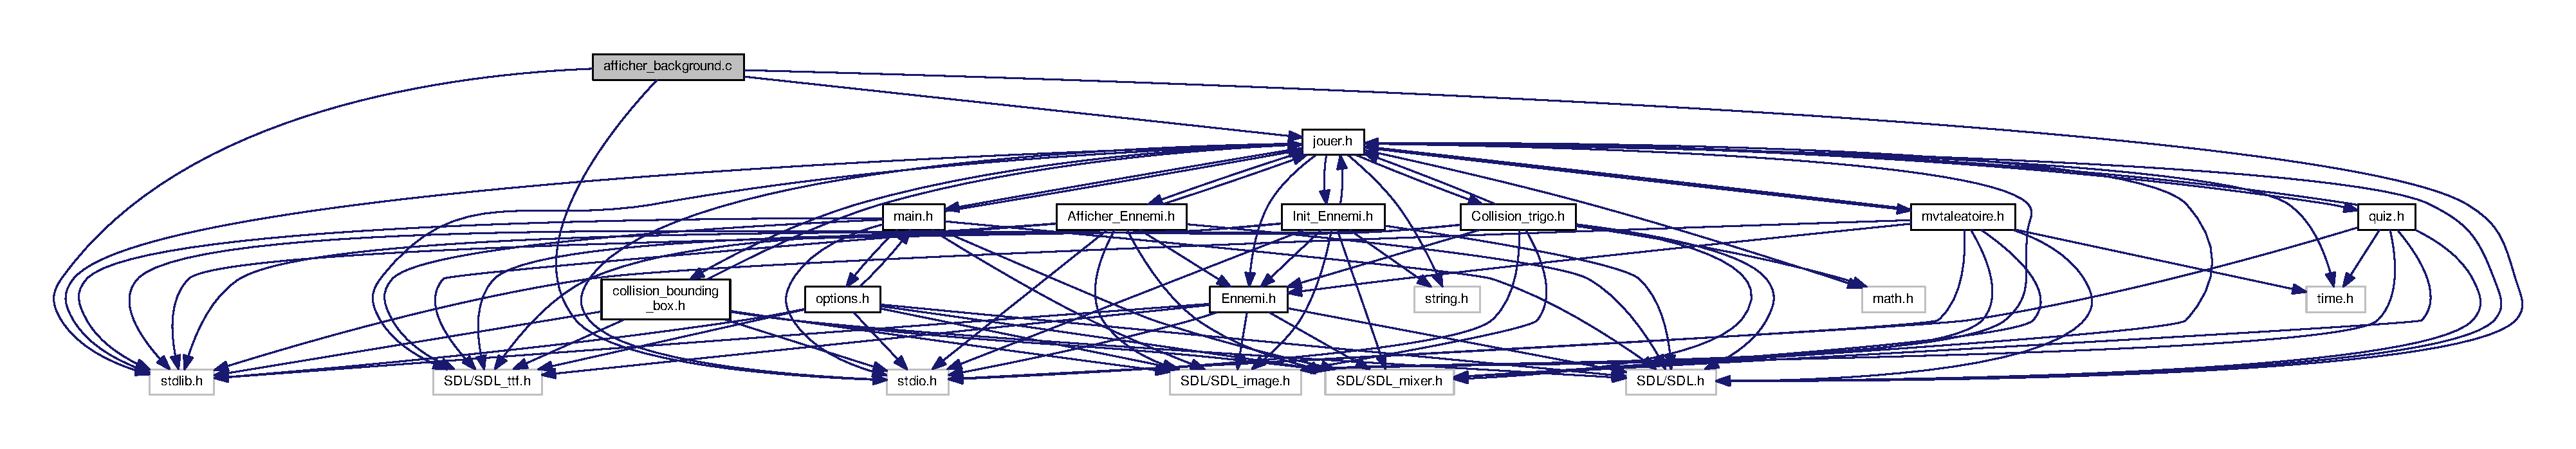
\includegraphics[width=350pt]{afficher__background_8c__incl}
\end{center}
\end{figure}
\subsection*{Functions}
\begin{DoxyCompactItemize}
\item 
void \hyperlink{afficher__background_8c_ad5e245ac884b3a5bc774dca864a5e0c0}{afficher} (S\+D\+L\+\_\+\+Surface $\ast$ecran, \hyperlink{structbackground}{background} $\ast$b)
\end{DoxyCompactItemize}


\subsection{Function Documentation}
\index{afficher\+\_\+background.\+c@{afficher\+\_\+background.\+c}!afficher@{afficher}}
\index{afficher@{afficher}!afficher\+\_\+background.\+c@{afficher\+\_\+background.\+c}}
\subsubsection[{\texorpdfstring{afficher(\+S\+D\+L\+\_\+\+Surface $\ast$ecran, background $\ast$b)}{afficher(SDL_Surface *ecran, background *b)}}]{\setlength{\rightskip}{0pt plus 5cm}void afficher (
\begin{DoxyParamCaption}
\item[{S\+D\+L\+\_\+\+Surface $\ast$}]{ecran, }
\item[{{\bf background} $\ast$}]{b}
\end{DoxyParamCaption}
)}\hypertarget{afficher__background_8c_ad5e245ac884b3a5bc774dca864a5e0c0}{}\label{afficher__background_8c_ad5e245ac884b3a5bc774dca864a5e0c0}


Here is the caller graph for this function\+:
\nopagebreak
\begin{figure}[H]
\begin{center}
\leavevmode
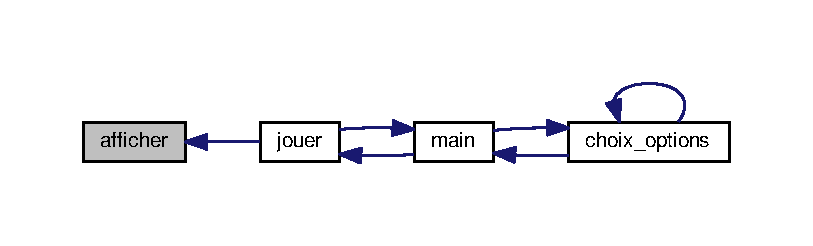
\includegraphics[width=350pt]{afficher__background_8c_ad5e245ac884b3a5bc774dca864a5e0c0_icgraph}
\end{center}
\end{figure}



\hypertarget{Afficher__Ennemi_8c}{}\section{Afficher\+\_\+\+Ennemi.\+c File Reference}
\label{Afficher__Ennemi_8c}\index{Afficher\+\_\+\+Ennemi.\+c@{Afficher\+\_\+\+Ennemi.\+c}}
{\ttfamily \#include $<$stdlib.\+h$>$}\\*
{\ttfamily \#include $<$stdio.\+h$>$}\\*
{\ttfamily \#include $<$S\+D\+L/\+S\+D\+L.\+h$>$}\\*
{\ttfamily \#include \char`\"{}Afficher\+\_\+\+Ennemi.\+h\char`\"{}}\\*
Include dependency graph for Afficher\+\_\+\+Ennemi.\+c\+:
\nopagebreak
\begin{figure}[H]
\begin{center}
\leavevmode
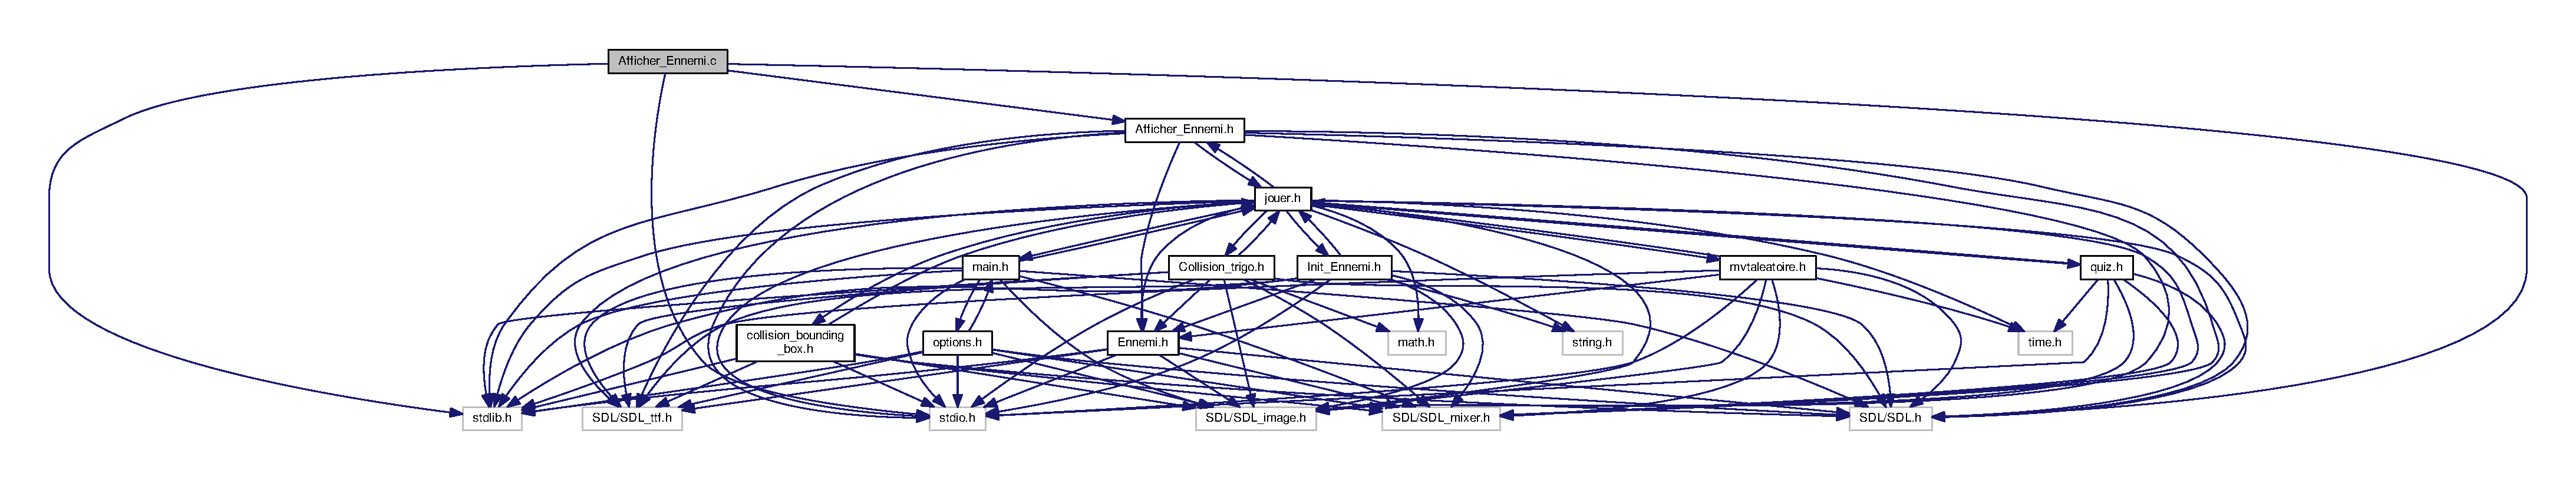
\includegraphics[width=350pt]{Afficher__Ennemi_8c__incl}
\end{center}
\end{figure}
\subsection*{Functions}
\begin{DoxyCompactItemize}
\item 
void \hyperlink{Afficher__Ennemi_8c_a5bd3b2cfb590a56ce994b524cd23e1aa}{Afficher\+\_\+\+Ennemi} (\hyperlink{structEnnemi}{Ennemi} Mob, S\+D\+L\+\_\+\+Surface $\ast$ecran)
\end{DoxyCompactItemize}


\subsection{Function Documentation}
\index{Afficher\+\_\+\+Ennemi.\+c@{Afficher\+\_\+\+Ennemi.\+c}!Afficher\+\_\+\+Ennemi@{Afficher\+\_\+\+Ennemi}}
\index{Afficher\+\_\+\+Ennemi@{Afficher\+\_\+\+Ennemi}!Afficher\+\_\+\+Ennemi.\+c@{Afficher\+\_\+\+Ennemi.\+c}}
\subsubsection[{\texorpdfstring{Afficher\+\_\+\+Ennemi(\+Ennemi Mob, S\+D\+L\+\_\+\+Surface $\ast$ecran)}{Afficher_Ennemi(Ennemi Mob, SDL_Surface *ecran)}}]{\setlength{\rightskip}{0pt plus 5cm}void Afficher\+\_\+\+Ennemi (
\begin{DoxyParamCaption}
\item[{{\bf Ennemi}}]{Mob, }
\item[{S\+D\+L\+\_\+\+Surface $\ast$}]{ecran}
\end{DoxyParamCaption}
)}\hypertarget{Afficher__Ennemi_8c_a5bd3b2cfb590a56ce994b524cd23e1aa}{}\label{Afficher__Ennemi_8c_a5bd3b2cfb590a56ce994b524cd23e1aa}


Here is the caller graph for this function\+:
\nopagebreak
\begin{figure}[H]
\begin{center}
\leavevmode
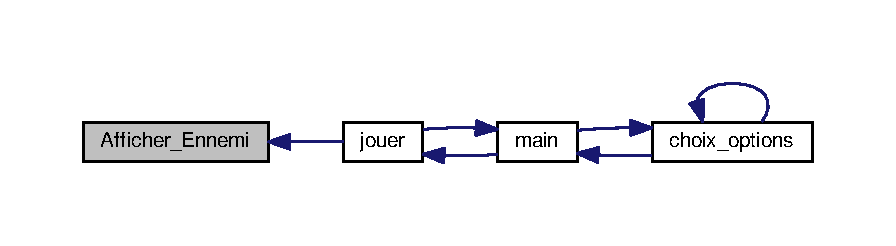
\includegraphics[width=350pt]{Afficher__Ennemi_8c_a5bd3b2cfb590a56ce994b524cd23e1aa_icgraph}
\end{center}
\end{figure}



\hypertarget{Afficher__Ennemi_8h}{}\section{Afficher\+\_\+\+Ennemi.\+h File Reference}
\label{Afficher__Ennemi_8h}\index{Afficher\+\_\+\+Ennemi.\+h@{Afficher\+\_\+\+Ennemi.\+h}}
{\ttfamily \#include $<$stdlib.\+h$>$}\\*
{\ttfamily \#include $<$stdio.\+h$>$}\\*
{\ttfamily \#include $<$S\+D\+L/\+S\+D\+L.\+h$>$}\\*
{\ttfamily \#include $<$S\+D\+L/\+S\+D\+L\+\_\+image.\+h$>$}\\*
{\ttfamily \#include $<$S\+D\+L/\+S\+D\+L\+\_\+mixer.\+h$>$}\\*
{\ttfamily \#include $<$S\+D\+L/\+S\+D\+L\+\_\+ttf.\+h$>$}\\*
{\ttfamily \#include \char`\"{}Ennemi.\+h\char`\"{}}\\*
{\ttfamily \#include \char`\"{}jouer.\+h\char`\"{}}\\*
Include dependency graph for Afficher\+\_\+\+Ennemi.\+h\+:
\nopagebreak
\begin{figure}[H]
\begin{center}
\leavevmode
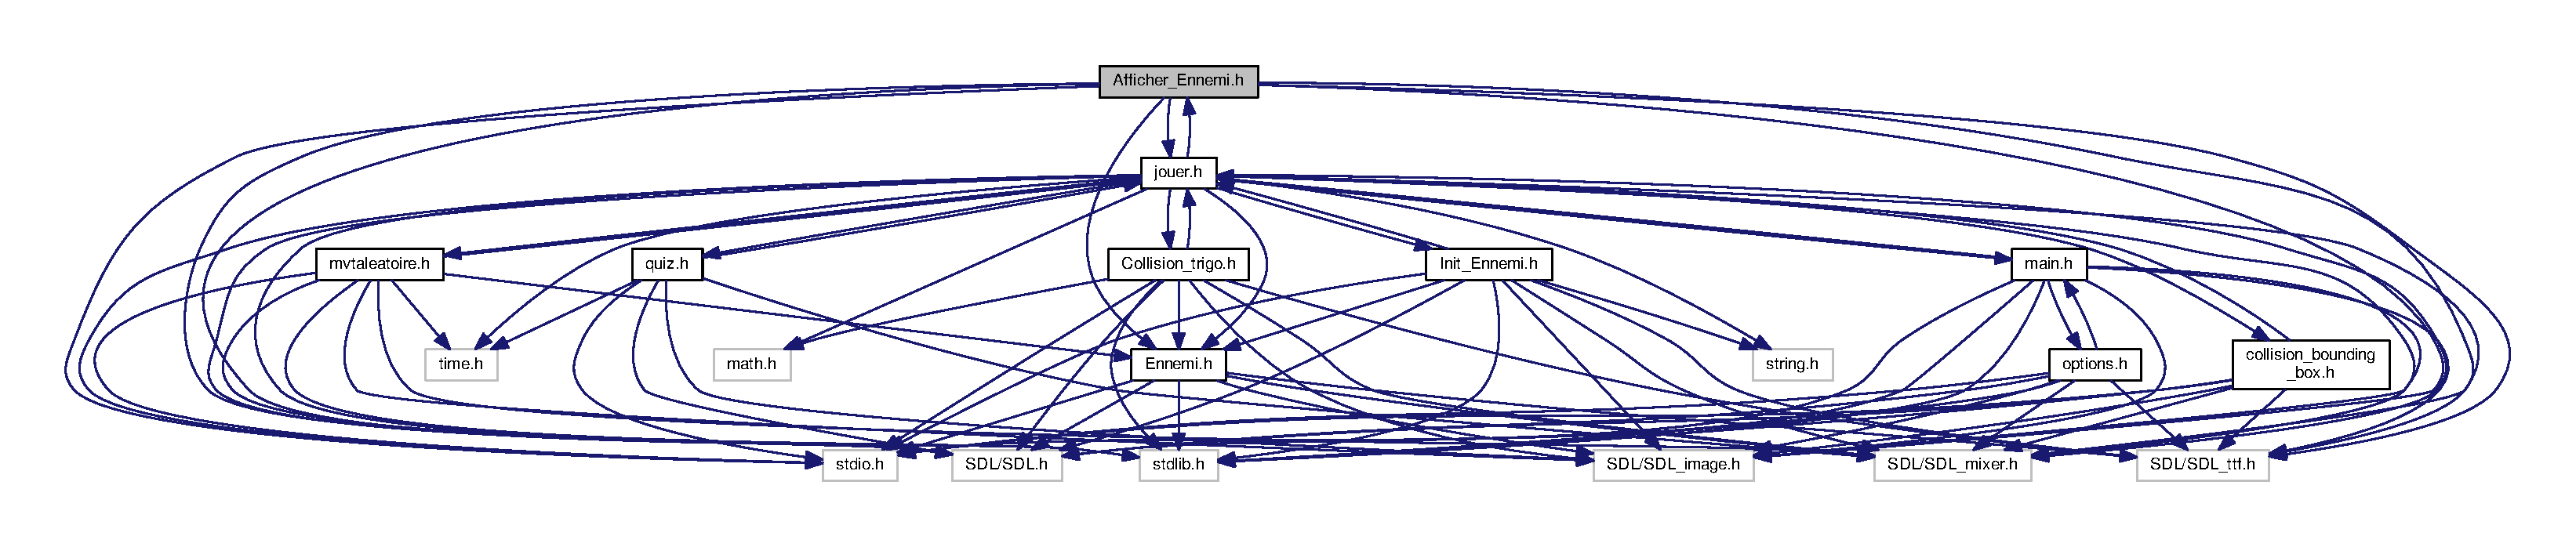
\includegraphics[width=350pt]{Afficher__Ennemi_8h__incl}
\end{center}
\end{figure}
This graph shows which files directly or indirectly include this file\+:
\nopagebreak
\begin{figure}[H]
\begin{center}
\leavevmode
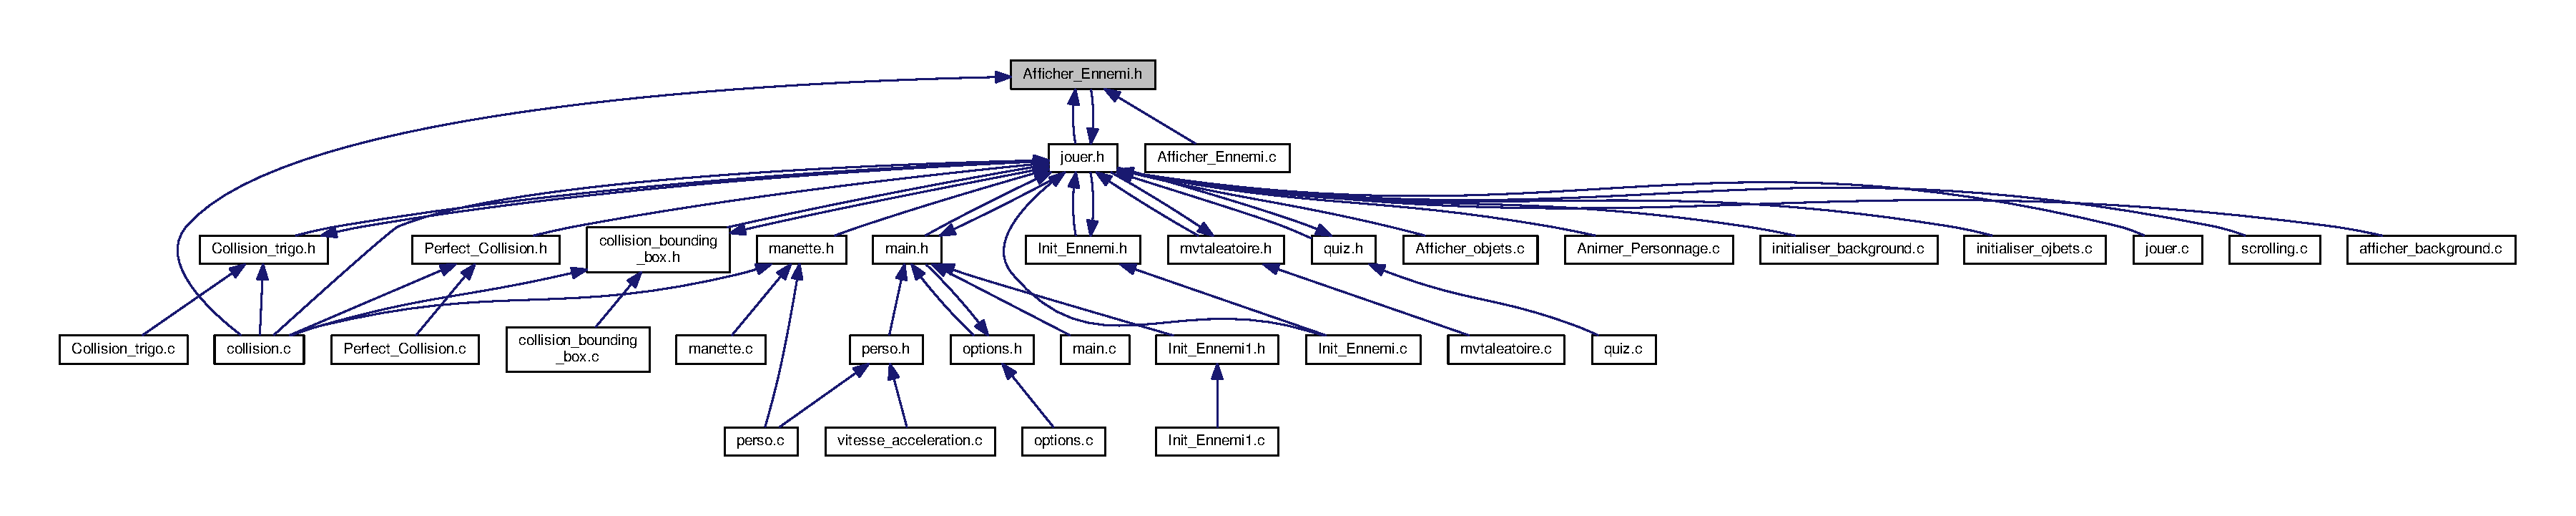
\includegraphics[width=350pt]{Afficher__Ennemi_8h__dep__incl}
\end{center}
\end{figure}
\subsection*{Functions}
\begin{DoxyCompactItemize}
\item 
void \hyperlink{Afficher__Ennemi_8h_a5bd3b2cfb590a56ce994b524cd23e1aa}{Afficher\+\_\+\+Ennemi} (\hyperlink{structEnnemi}{Ennemi} Mob, S\+D\+L\+\_\+\+Surface $\ast$ecran)
\end{DoxyCompactItemize}


\subsection{Function Documentation}
\index{Afficher\+\_\+\+Ennemi.\+h@{Afficher\+\_\+\+Ennemi.\+h}!Afficher\+\_\+\+Ennemi@{Afficher\+\_\+\+Ennemi}}
\index{Afficher\+\_\+\+Ennemi@{Afficher\+\_\+\+Ennemi}!Afficher\+\_\+\+Ennemi.\+h@{Afficher\+\_\+\+Ennemi.\+h}}
\subsubsection[{\texorpdfstring{Afficher\+\_\+\+Ennemi(\+Ennemi Mob, S\+D\+L\+\_\+\+Surface $\ast$ecran)}{Afficher_Ennemi(Ennemi Mob, SDL_Surface *ecran)}}]{\setlength{\rightskip}{0pt plus 5cm}void Afficher\+\_\+\+Ennemi (
\begin{DoxyParamCaption}
\item[{{\bf Ennemi}}]{Mob, }
\item[{S\+D\+L\+\_\+\+Surface $\ast$}]{ecran}
\end{DoxyParamCaption}
)}\hypertarget{Afficher__Ennemi_8h_a5bd3b2cfb590a56ce994b524cd23e1aa}{}\label{Afficher__Ennemi_8h_a5bd3b2cfb590a56ce994b524cd23e1aa}

\hypertarget{Afficher__objets_8c}{}\section{Afficher\+\_\+objets.\+c File Reference}
\label{Afficher__objets_8c}\index{Afficher\+\_\+objets.\+c@{Afficher\+\_\+objets.\+c}}
{\ttfamily \#include $<$stdlib.\+h$>$}\\*
{\ttfamily \#include $<$stdio.\+h$>$}\\*
{\ttfamily \#include $<$S\+D\+L/\+S\+D\+L.\+h$>$}\\*
{\ttfamily \#include \char`\"{}jouer.\+h\char`\"{}}\\*
Include dependency graph for Afficher\+\_\+objets.\+c\+:
\nopagebreak
\begin{figure}[H]
\begin{center}
\leavevmode
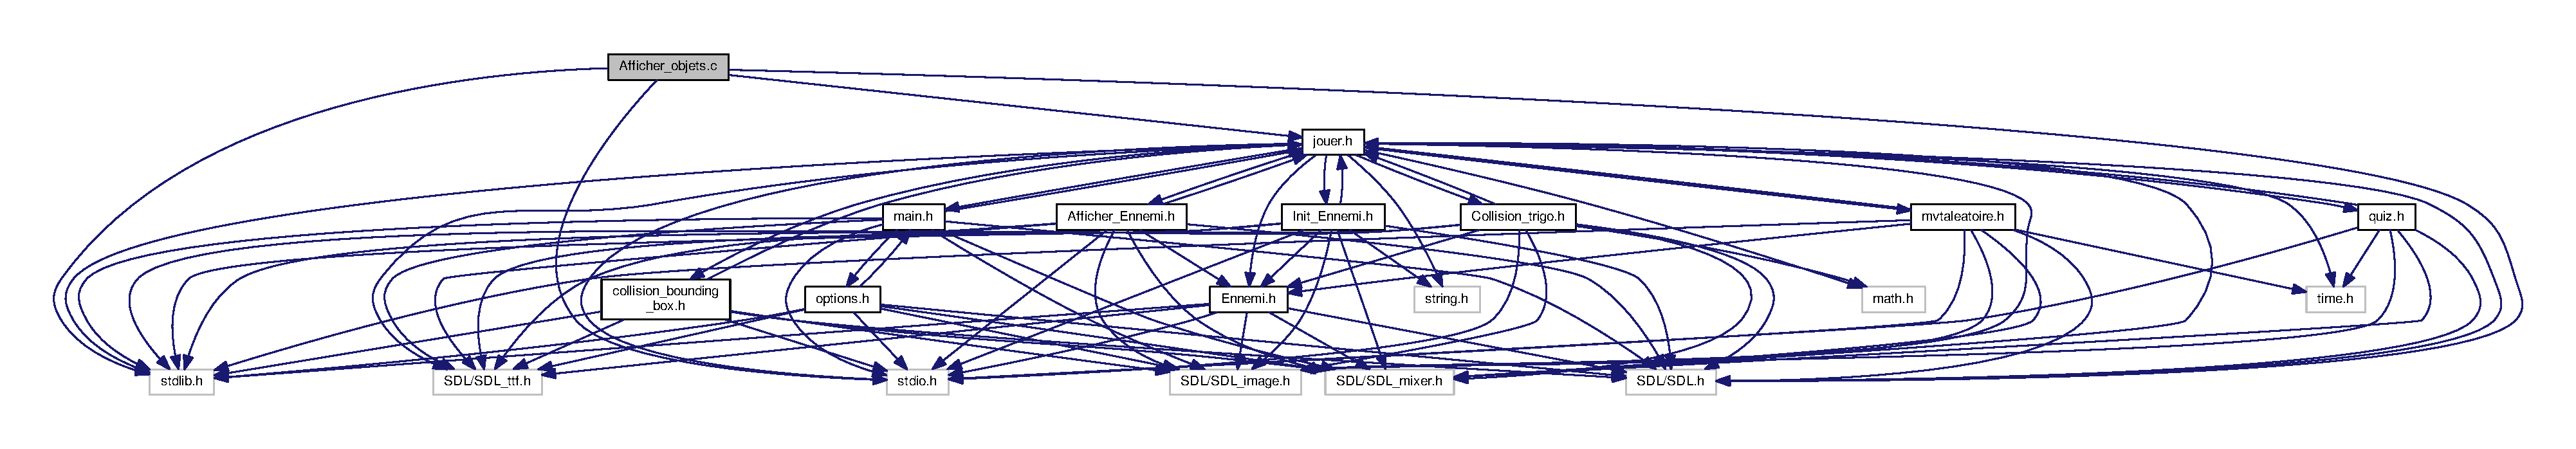
\includegraphics[width=350pt]{Afficher__objets_8c__incl}
\end{center}
\end{figure}
\subsection*{Functions}
\begin{DoxyCompactItemize}
\item 
void \hyperlink{Afficher__objets_8c_a42cab3047c025df170f86a167a498c40}{afficherobjet} (\hyperlink{structEO}{EO} $\ast$ob, \hyperlink{structEO}{EO} $\ast$clef, \hyperlink{structEO}{EO} $\ast$porte, \hyperlink{structEO}{EO} $\ast$piste, S\+D\+L\+\_\+\+Surface $\ast$ecran, \hyperlink{structbackground}{background} $\ast$b)
\end{DoxyCompactItemize}


\subsection{Function Documentation}
\index{Afficher\+\_\+objets.\+c@{Afficher\+\_\+objets.\+c}!afficherobjet@{afficherobjet}}
\index{afficherobjet@{afficherobjet}!Afficher\+\_\+objets.\+c@{Afficher\+\_\+objets.\+c}}
\subsubsection[{\texorpdfstring{afficherobjet(\+E\+O $\ast$ob, E\+O $\ast$clef, E\+O $\ast$porte, E\+O $\ast$piste, S\+D\+L\+\_\+\+Surface $\ast$ecran, background $\ast$b)}{afficherobjet(EO *ob, EO *clef, EO *porte, EO *piste, SDL_Surface *ecran, background *b)}}]{\setlength{\rightskip}{0pt plus 5cm}void afficherobjet (
\begin{DoxyParamCaption}
\item[{{\bf EO} $\ast$}]{ob, }
\item[{{\bf EO} $\ast$}]{clef, }
\item[{{\bf EO} $\ast$}]{porte, }
\item[{{\bf EO} $\ast$}]{piste, }
\item[{S\+D\+L\+\_\+\+Surface $\ast$}]{ecran, }
\item[{{\bf background} $\ast$}]{b}
\end{DoxyParamCaption}
)}\hypertarget{Afficher__objets_8c_a42cab3047c025df170f86a167a498c40}{}\label{Afficher__objets_8c_a42cab3047c025df170f86a167a498c40}


Here is the caller graph for this function\+:
\nopagebreak
\begin{figure}[H]
\begin{center}
\leavevmode
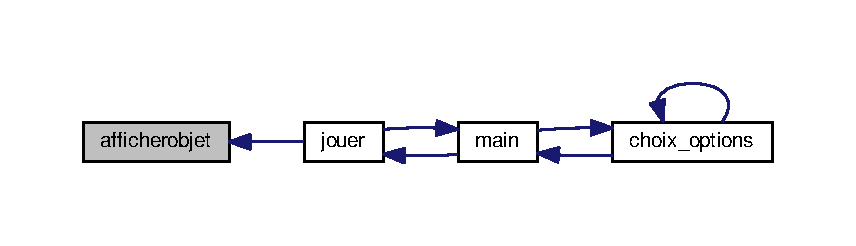
\includegraphics[width=350pt]{Afficher__objets_8c_a42cab3047c025df170f86a167a498c40_icgraph}
\end{center}
\end{figure}



\hypertarget{Animer__Personnage_8c}{}\section{Animer\+\_\+\+Personnage.\+c File Reference}
\label{Animer__Personnage_8c}\index{Animer\+\_\+\+Personnage.\+c@{Animer\+\_\+\+Personnage.\+c}}
{\ttfamily \#include $<$stdlib.\+h$>$}\\*
{\ttfamily \#include $<$stdio.\+h$>$}\\*
{\ttfamily \#include $<$S\+D\+L/\+S\+D\+L.\+h$>$}\\*
{\ttfamily \#include \char`\"{}jouer.\+h\char`\"{}}\\*
Include dependency graph for Animer\+\_\+\+Personnage.\+c\+:
\nopagebreak
\begin{figure}[H]
\begin{center}
\leavevmode
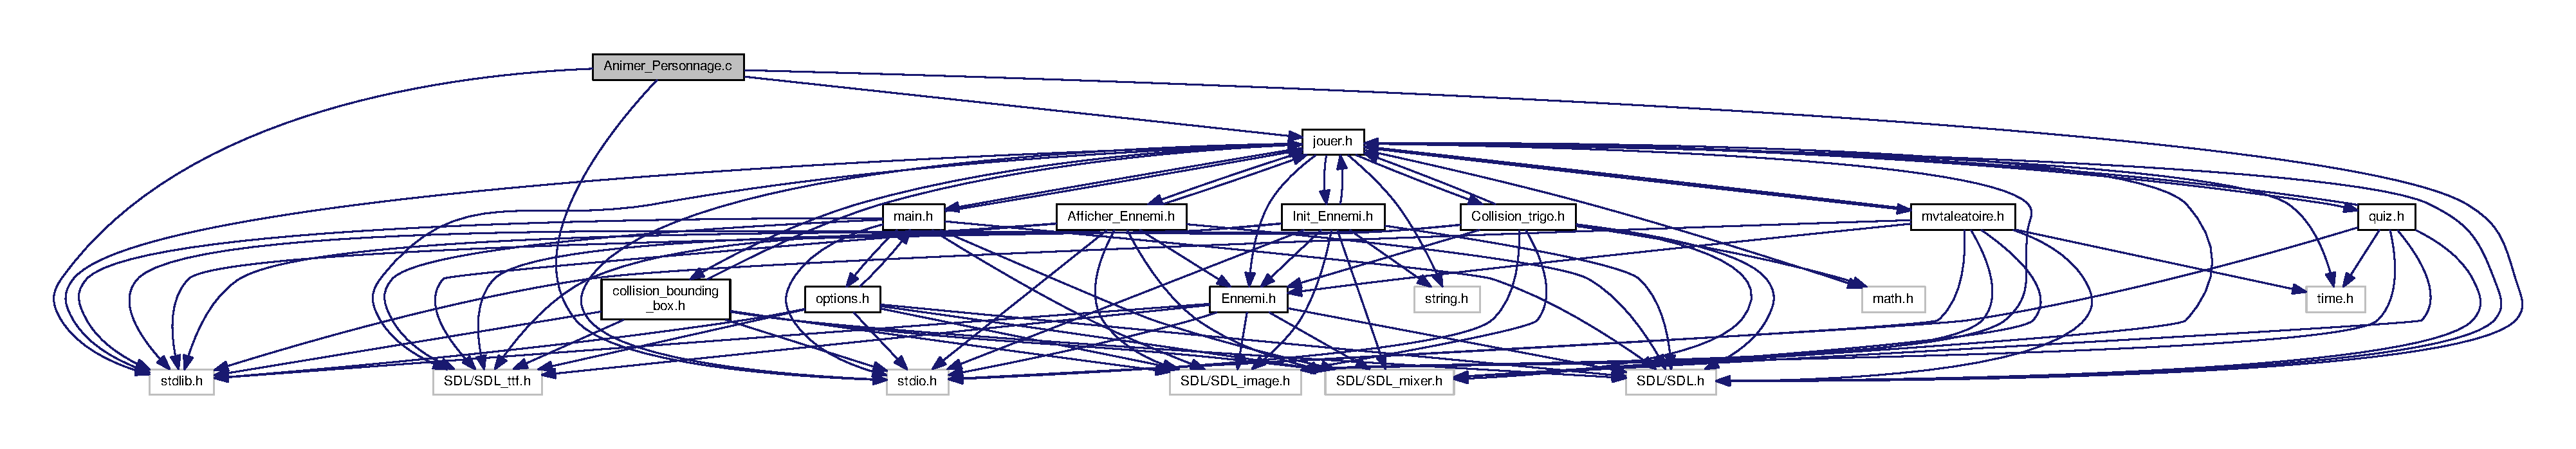
\includegraphics[width=350pt]{Animer__Personnage_8c__incl}
\end{center}
\end{figure}
\subsection*{Functions}
\begin{DoxyCompactItemize}
\item 
void \hyperlink{Animer__Personnage_8c_a3dc3993bdcecc71ad5576c072f25e29d}{Animer\+\_\+\+Personnage} (int $\ast$frametime, int nmb\+\_\+frame, int $\ast$frame, \hyperlink{structPlayer}{Player} $\ast$hero, \hyperlink{jouer_8h_a224b9163917ac32fc95a60d8c1eec3aa}{Direction} $\ast$Sens, \hyperlink{jouer_8h_a767b7a63d7677f92d697621b4166af1b}{Etat} $\ast$State)
\end{DoxyCompactItemize}


\subsection{Function Documentation}
\index{Animer\+\_\+\+Personnage.\+c@{Animer\+\_\+\+Personnage.\+c}!Animer\+\_\+\+Personnage@{Animer\+\_\+\+Personnage}}
\index{Animer\+\_\+\+Personnage@{Animer\+\_\+\+Personnage}!Animer\+\_\+\+Personnage.\+c@{Animer\+\_\+\+Personnage.\+c}}
\subsubsection[{\texorpdfstring{Animer\+\_\+\+Personnage(int $\ast$frametime, int nmb\+\_\+frame, int $\ast$frame, Player $\ast$hero, Direction $\ast$\+Sens, Etat $\ast$\+State)}{Animer_Personnage(int *frametime, int nmb_frame, int *frame, Player *hero, Direction *Sens, Etat *State)}}]{\setlength{\rightskip}{0pt plus 5cm}void Animer\+\_\+\+Personnage (
\begin{DoxyParamCaption}
\item[{int $\ast$}]{frametime, }
\item[{int}]{nmb\+\_\+frame, }
\item[{int $\ast$}]{frame, }
\item[{{\bf Player} $\ast$}]{hero, }
\item[{{\bf Direction} $\ast$}]{Sens, }
\item[{{\bf Etat} $\ast$}]{State}
\end{DoxyParamCaption}
)}\hypertarget{Animer__Personnage_8c_a3dc3993bdcecc71ad5576c072f25e29d}{}\label{Animer__Personnage_8c_a3dc3993bdcecc71ad5576c072f25e29d}


Here is the caller graph for this function\+:
\nopagebreak
\begin{figure}[H]
\begin{center}
\leavevmode
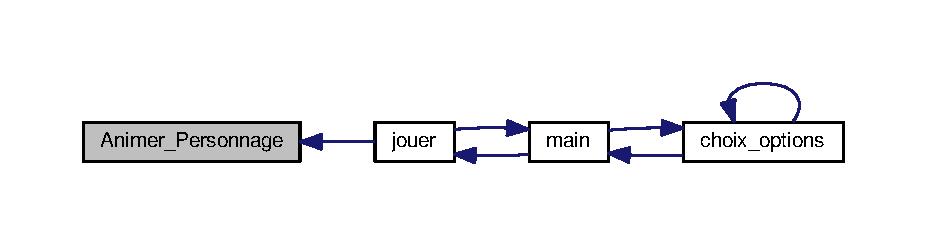
\includegraphics[width=350pt]{Animer__Personnage_8c_a3dc3993bdcecc71ad5576c072f25e29d_icgraph}
\end{center}
\end{figure}



\hypertarget{Animer__Personnage_8h}{}\section{Animer\+\_\+\+Personnage.\+h File Reference}
\label{Animer__Personnage_8h}\index{Animer\+\_\+\+Personnage.\+h@{Animer\+\_\+\+Personnage.\+h}}
{\ttfamily \#include $<$stdlib.\+h$>$}\\*
{\ttfamily \#include $<$stdio.\+h$>$}\\*
{\ttfamily \#include $<$math.\+h$>$}\\*
{\ttfamily \#include $<$string.\+h$>$}\\*
{\ttfamily \#include $<$S\+D\+L/\+S\+D\+L.\+h$>$}\\*
{\ttfamily \#include $<$S\+D\+L/\+S\+D\+L\+\_\+image.\+h$>$}\\*
{\ttfamily \#include $<$S\+D\+L/\+S\+D\+L\+\_\+mixer.\+h$>$}\\*
{\ttfamily \#include $<$S\+D\+L/\+S\+D\+L\+\_\+ttf.\+h$>$}\\*
Include dependency graph for Animer\+\_\+\+Personnage.\+h\+:\nopagebreak
\begin{figure}[H]
\begin{center}
\leavevmode
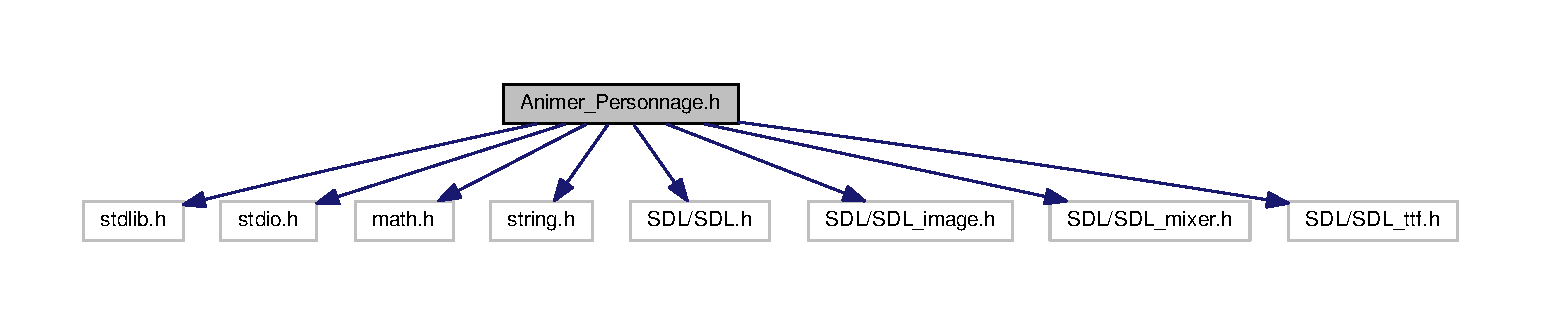
\includegraphics[width=350pt]{Animer__Personnage_8h__incl}
\end{center}
\end{figure}

\hypertarget{collision_8c}{}\section{collision.\+c File Reference}
\label{collision_8c}\index{collision.\+c@{collision.\+c}}
{\ttfamily \#include $<$stdlib.\+h$>$}\\*
{\ttfamily \#include $<$stdio.\+h$>$}\\*
{\ttfamily \#include $<$S\+D\+L/\+S\+D\+L.\+h$>$}\\*
{\ttfamily \#include \char`\"{}jouer.\+h\char`\"{}}\\*
{\ttfamily \#include \char`\"{}collision\+\_\+bounding\+\_\+box.\+h\char`\"{}}\\*
{\ttfamily \#include \char`\"{}Collision\+\_\+trigo.\+h\char`\"{}}\\*
{\ttfamily \#include \char`\"{}Ennemi.\+h\char`\"{}}\\*
{\ttfamily \#include \char`\"{}Afficher\+\_\+\+Ennemi.\+h\char`\"{}}\\*
{\ttfamily \#include \char`\"{}Perfect\+\_\+\+Collision.\+h\char`\"{}}\\*
{\ttfamily \#include \char`\"{}manette.\+h\char`\"{}}\\*
Include dependency graph for collision.\+c\+:
\nopagebreak
\begin{figure}[H]
\begin{center}
\leavevmode
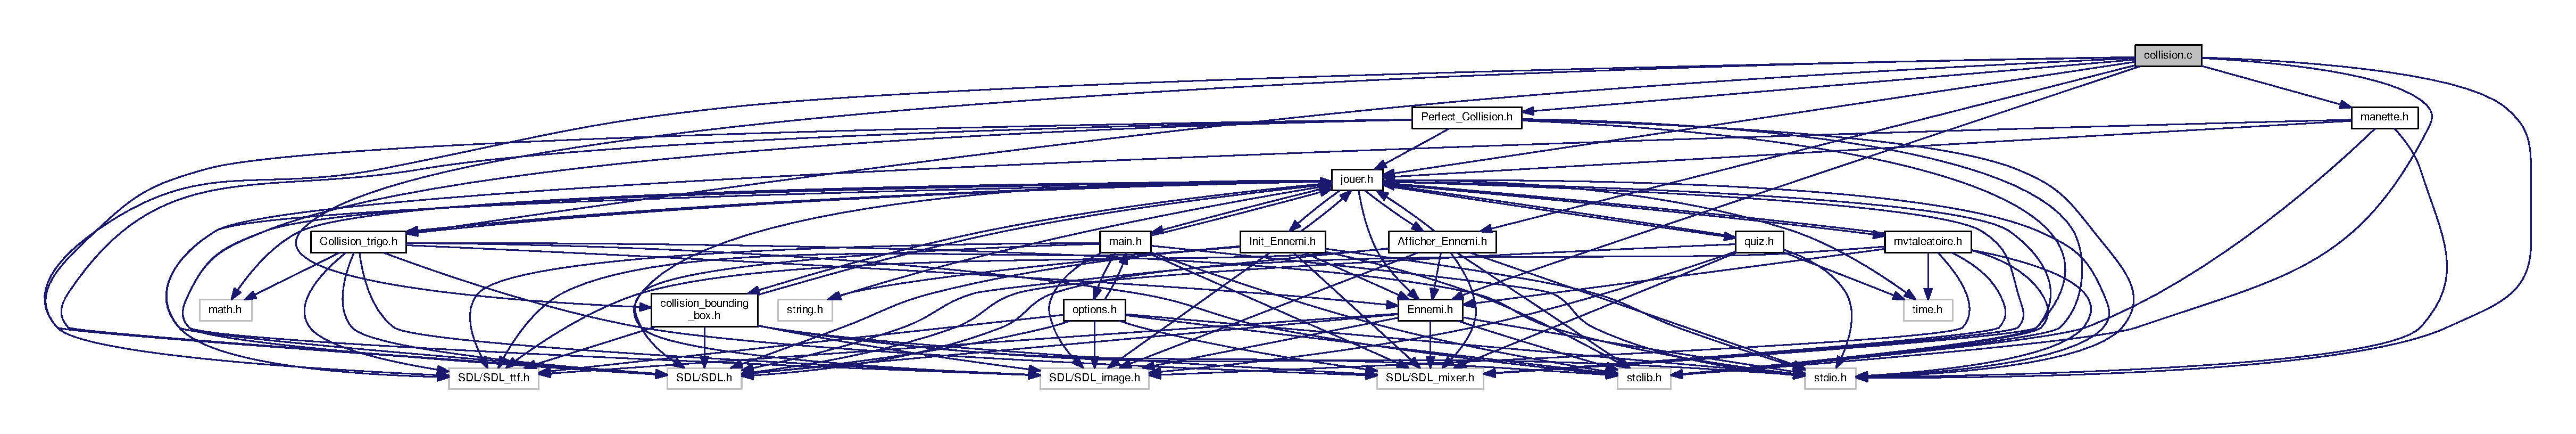
\includegraphics[width=350pt]{collision_8c__incl}
\end{center}
\end{figure}
\subsection*{Functions}
\begin{DoxyCompactItemize}
\item 
int \hyperlink{collision_8c_a1201e4f88c0ee7608ca131ce01681997}{collisionall} (\hyperlink{structEO}{EO} $\ast$ob, \hyperlink{structEO}{EO} clef, \hyperlink{structEO}{EO} porte, \hyperlink{structEO}{EO} piste, \hyperlink{structPlayer}{Player} $\ast$hero, int $\ast$vie, int $\ast$score, \hyperlink{jouer_8h_a224b9163917ac32fc95a60d8c1eec3aa}{Direction} Sens, \hyperlink{jouer_8h_a767b7a63d7677f92d697621b4166af1b}{Etat} State, \hyperlink{structEnnemi}{Ennemi} Mob\mbox{[}$\,$\mbox{]}, \hyperlink{structCoordinate}{Coordinate} C, S\+D\+L\+\_\+\+Surface $\ast$Background)
\end{DoxyCompactItemize}


\subsection{Function Documentation}
\index{collision.\+c@{collision.\+c}!collisionall@{collisionall}}
\index{collisionall@{collisionall}!collision.\+c@{collision.\+c}}
\subsubsection[{\texorpdfstring{collisionall(\+E\+O $\ast$ob, E\+O clef, E\+O porte, E\+O piste, Player $\ast$hero, int $\ast$vie, int $\ast$score, Direction Sens, Etat State, Ennemi Mob[], Coordinate C, S\+D\+L\+\_\+\+Surface $\ast$\+Background)}{collisionall(EO *ob, EO clef, EO porte, EO piste, Player *hero, int *vie, int *score, Direction Sens, Etat State, Ennemi Mob[], Coordinate C, SDL_Surface *Background)}}]{\setlength{\rightskip}{0pt plus 5cm}int collisionall (
\begin{DoxyParamCaption}
\item[{{\bf EO} $\ast$}]{ob, }
\item[{{\bf EO}}]{clef, }
\item[{{\bf EO}}]{porte, }
\item[{{\bf EO}}]{piste, }
\item[{{\bf Player} $\ast$}]{hero, }
\item[{int $\ast$}]{vie, }
\item[{int $\ast$}]{score, }
\item[{{\bf Direction}}]{Sens, }
\item[{{\bf Etat}}]{State, }
\item[{{\bf Ennemi}}]{Mob\mbox{[}$\,$\mbox{]}, }
\item[{{\bf Coordinate}}]{C, }
\item[{S\+D\+L\+\_\+\+Surface $\ast$}]{Background}
\end{DoxyParamCaption}
)}\hypertarget{collision_8c_a1201e4f88c0ee7608ca131ce01681997}{}\label{collision_8c_a1201e4f88c0ee7608ca131ce01681997}


Here is the call graph for this function\+:
\nopagebreak
\begin{figure}[H]
\begin{center}
\leavevmode
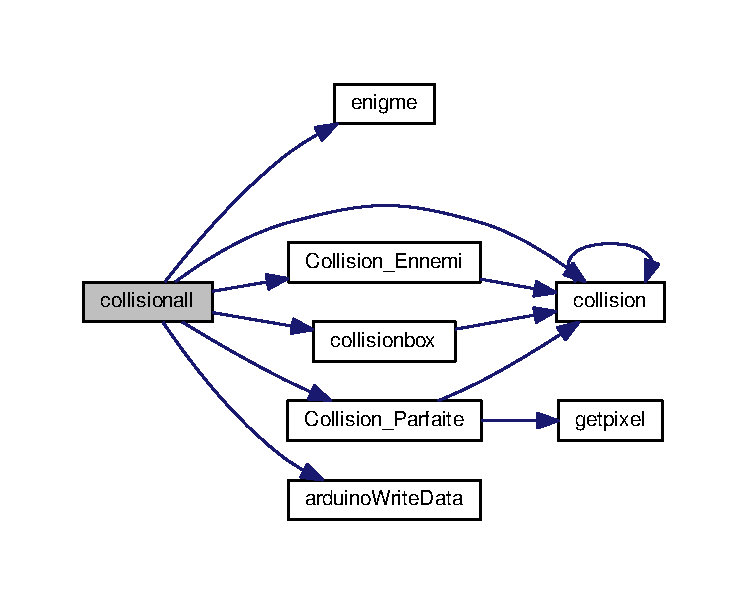
\includegraphics[width=350pt]{collision_8c_a1201e4f88c0ee7608ca131ce01681997_cgraph}
\end{center}
\end{figure}




Here is the caller graph for this function\+:
\nopagebreak
\begin{figure}[H]
\begin{center}
\leavevmode
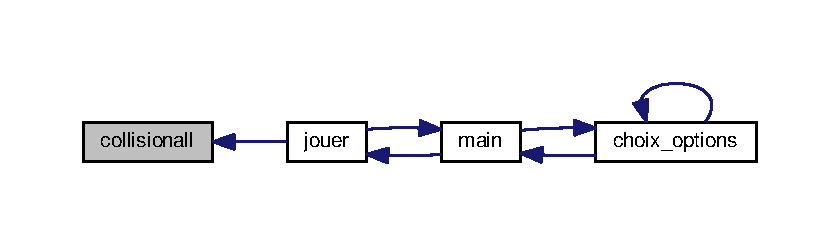
\includegraphics[width=350pt]{collision_8c_a1201e4f88c0ee7608ca131ce01681997_icgraph}
\end{center}
\end{figure}



\hypertarget{collision__bounding__box_8c}{}\section{collision\+\_\+bounding\+\_\+box.\+c File Reference}
\label{collision__bounding__box_8c}\index{collision\+\_\+bounding\+\_\+box.\+c@{collision\+\_\+bounding\+\_\+box.\+c}}
{\ttfamily \#include $<$stdlib.\+h$>$}\\*
{\ttfamily \#include $<$stdio.\+h$>$}\\*
{\ttfamily \#include $<$S\+D\+L/\+S\+D\+L.\+h$>$}\\*
{\ttfamily \#include \char`\"{}collision\+\_\+bounding\+\_\+box.\+h\char`\"{}}\\*
Include dependency graph for collision\+\_\+bounding\+\_\+box.\+c\+:
\nopagebreak
\begin{figure}[H]
\begin{center}
\leavevmode
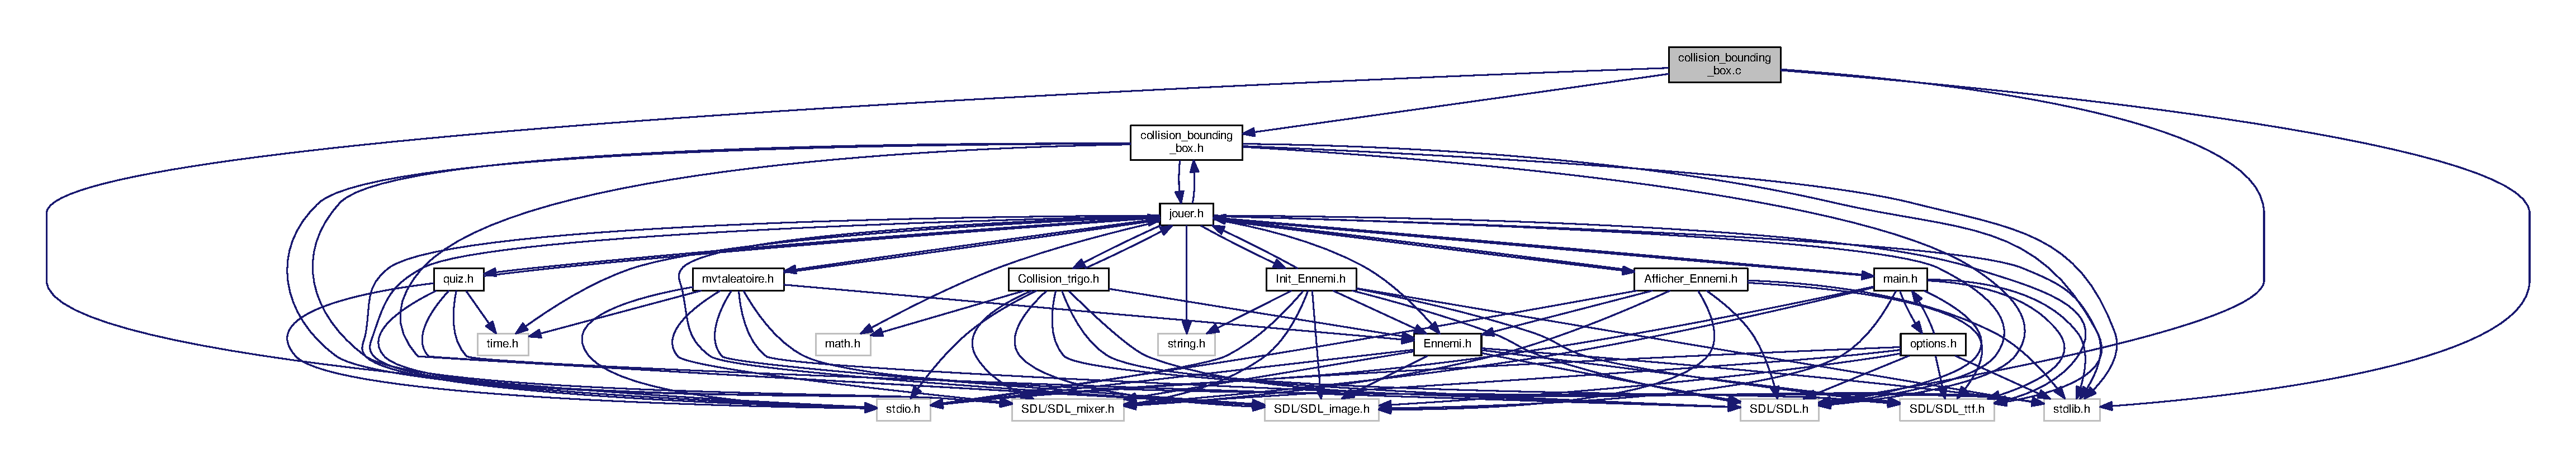
\includegraphics[width=350pt]{collision__bounding__box_8c__incl}
\end{center}
\end{figure}
\subsection*{Functions}
\begin{DoxyCompactItemize}
\item 
int \hyperlink{collision__bounding__box_8c_aaf6f1dec5bb7d4e93d8d580a8e550442}{collision} (S\+D\+L\+\_\+\+Surface $\ast$p, S\+D\+L\+\_\+\+Surface $\ast$e, S\+D\+L\+\_\+\+Rect perso, S\+D\+L\+\_\+\+Rect enemy)
\item 
int \hyperlink{collision__bounding__box_8c_aada0004db077b368ab0b29a7f0e74d72}{collisionbox} (S\+D\+L\+\_\+\+Surface $\ast$p, S\+D\+L\+\_\+\+Surface $\ast$o, S\+D\+L\+\_\+\+Rect perso, S\+D\+L\+\_\+\+Rect objet)
\end{DoxyCompactItemize}


\subsection{Function Documentation}
\index{collision\+\_\+bounding\+\_\+box.\+c@{collision\+\_\+bounding\+\_\+box.\+c}!collision@{collision}}
\index{collision@{collision}!collision\+\_\+bounding\+\_\+box.\+c@{collision\+\_\+bounding\+\_\+box.\+c}}
\subsubsection[{\texorpdfstring{collision(\+S\+D\+L\+\_\+\+Surface $\ast$p, S\+D\+L\+\_\+\+Surface $\ast$e, S\+D\+L\+\_\+\+Rect perso, S\+D\+L\+\_\+\+Rect enemy)}{collision(SDL_Surface *p, SDL_Surface *e, SDL_Rect perso, SDL_Rect enemy)}}]{\setlength{\rightskip}{0pt plus 5cm}int collision (
\begin{DoxyParamCaption}
\item[{S\+D\+L\+\_\+\+Surface $\ast$}]{p, }
\item[{S\+D\+L\+\_\+\+Surface $\ast$}]{e, }
\item[{S\+D\+L\+\_\+\+Rect}]{perso, }
\item[{S\+D\+L\+\_\+\+Rect}]{enemy}
\end{DoxyParamCaption}
)}\hypertarget{collision__bounding__box_8c_aaf6f1dec5bb7d4e93d8d580a8e550442}{}\label{collision__bounding__box_8c_aaf6f1dec5bb7d4e93d8d580a8e550442}


Here is the call graph for this function\+:\nopagebreak
\begin{figure}[H]
\begin{center}
\leavevmode
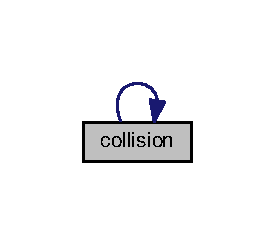
\includegraphics[width=132pt]{collision__bounding__box_8c_aaf6f1dec5bb7d4e93d8d580a8e550442_cgraph}
\end{center}
\end{figure}




Here is the caller graph for this function\+:
\nopagebreak
\begin{figure}[H]
\begin{center}
\leavevmode
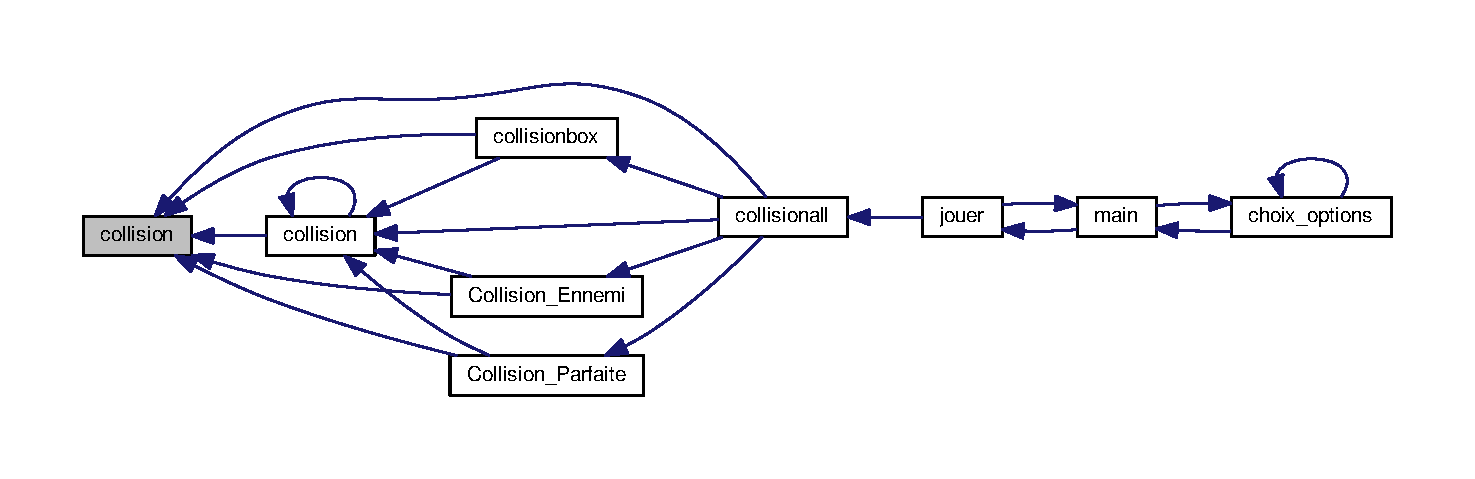
\includegraphics[width=350pt]{collision__bounding__box_8c_aaf6f1dec5bb7d4e93d8d580a8e550442_icgraph}
\end{center}
\end{figure}


\index{collision\+\_\+bounding\+\_\+box.\+c@{collision\+\_\+bounding\+\_\+box.\+c}!collisionbox@{collisionbox}}
\index{collisionbox@{collisionbox}!collision\+\_\+bounding\+\_\+box.\+c@{collision\+\_\+bounding\+\_\+box.\+c}}
\subsubsection[{\texorpdfstring{collisionbox(\+S\+D\+L\+\_\+\+Surface $\ast$p, S\+D\+L\+\_\+\+Surface $\ast$o, S\+D\+L\+\_\+\+Rect perso, S\+D\+L\+\_\+\+Rect objet)}{collisionbox(SDL_Surface *p, SDL_Surface *o, SDL_Rect perso, SDL_Rect objet)}}]{\setlength{\rightskip}{0pt plus 5cm}int collisionbox (
\begin{DoxyParamCaption}
\item[{S\+D\+L\+\_\+\+Surface $\ast$}]{p, }
\item[{S\+D\+L\+\_\+\+Surface $\ast$}]{o, }
\item[{S\+D\+L\+\_\+\+Rect}]{perso, }
\item[{S\+D\+L\+\_\+\+Rect}]{objet}
\end{DoxyParamCaption}
)}\hypertarget{collision__bounding__box_8c_aada0004db077b368ab0b29a7f0e74d72}{}\label{collision__bounding__box_8c_aada0004db077b368ab0b29a7f0e74d72}


Here is the call graph for this function\+:\nopagebreak
\begin{figure}[H]
\begin{center}
\leavevmode
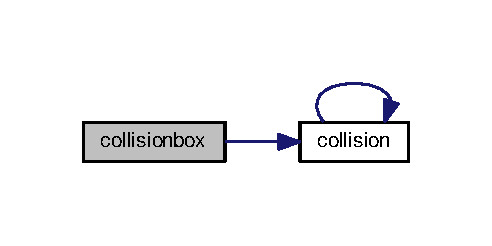
\includegraphics[width=236pt]{collision__bounding__box_8c_aada0004db077b368ab0b29a7f0e74d72_cgraph}
\end{center}
\end{figure}




Here is the caller graph for this function\+:
\nopagebreak
\begin{figure}[H]
\begin{center}
\leavevmode
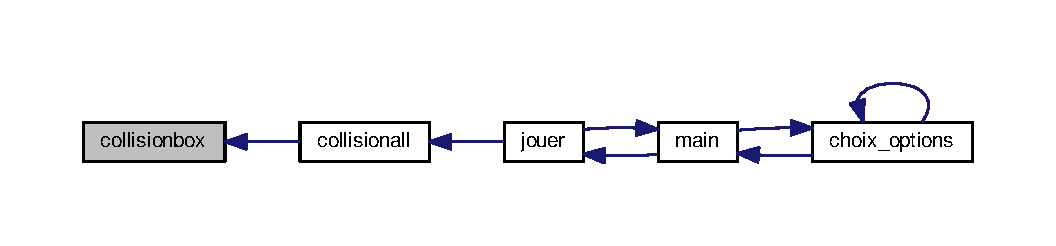
\includegraphics[width=350pt]{collision__bounding__box_8c_aada0004db077b368ab0b29a7f0e74d72_icgraph}
\end{center}
\end{figure}



\hypertarget{collision__bounding__box_8h}{}\section{collision\+\_\+bounding\+\_\+box.\+h File Reference}
\label{collision__bounding__box_8h}\index{collision\+\_\+bounding\+\_\+box.\+h@{collision\+\_\+bounding\+\_\+box.\+h}}
{\ttfamily \#include $<$stdlib.\+h$>$}\\*
{\ttfamily \#include $<$stdio.\+h$>$}\\*
{\ttfamily \#include $<$S\+D\+L/\+S\+D\+L.\+h$>$}\\*
{\ttfamily \#include $<$S\+D\+L/\+S\+D\+L\+\_\+image.\+h$>$}\\*
{\ttfamily \#include $<$S\+D\+L/\+S\+D\+L\+\_\+mixer.\+h$>$}\\*
{\ttfamily \#include $<$S\+D\+L/\+S\+D\+L\+\_\+ttf.\+h$>$}\\*
{\ttfamily \#include \char`\"{}jouer.\+h\char`\"{}}\\*
Include dependency graph for collision\+\_\+bounding\+\_\+box.\+h\+:
\nopagebreak
\begin{figure}[H]
\begin{center}
\leavevmode
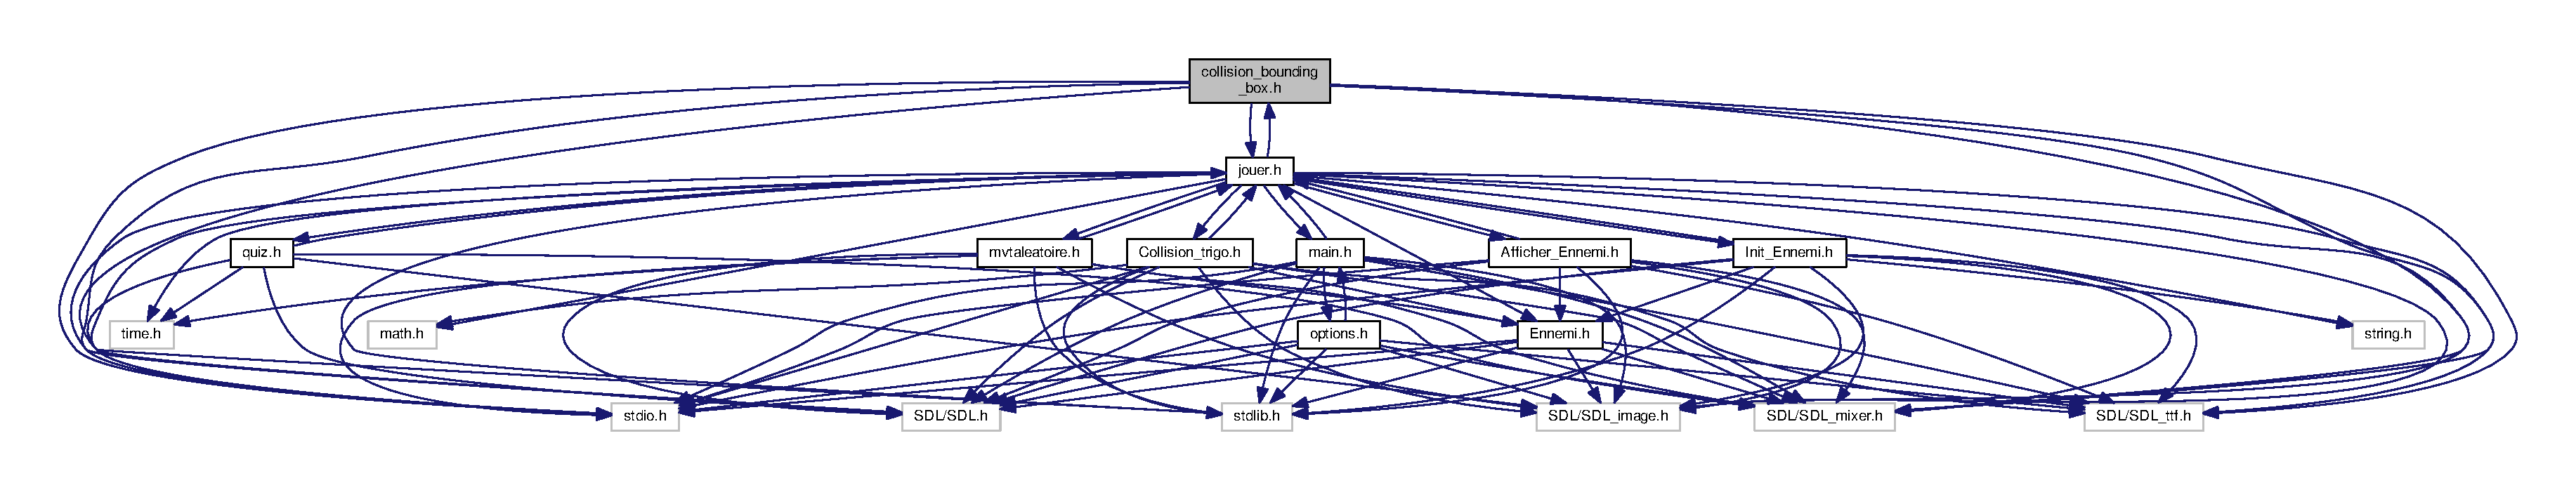
\includegraphics[width=350pt]{collision__bounding__box_8h__incl}
\end{center}
\end{figure}
This graph shows which files directly or indirectly include this file\+:
\nopagebreak
\begin{figure}[H]
\begin{center}
\leavevmode
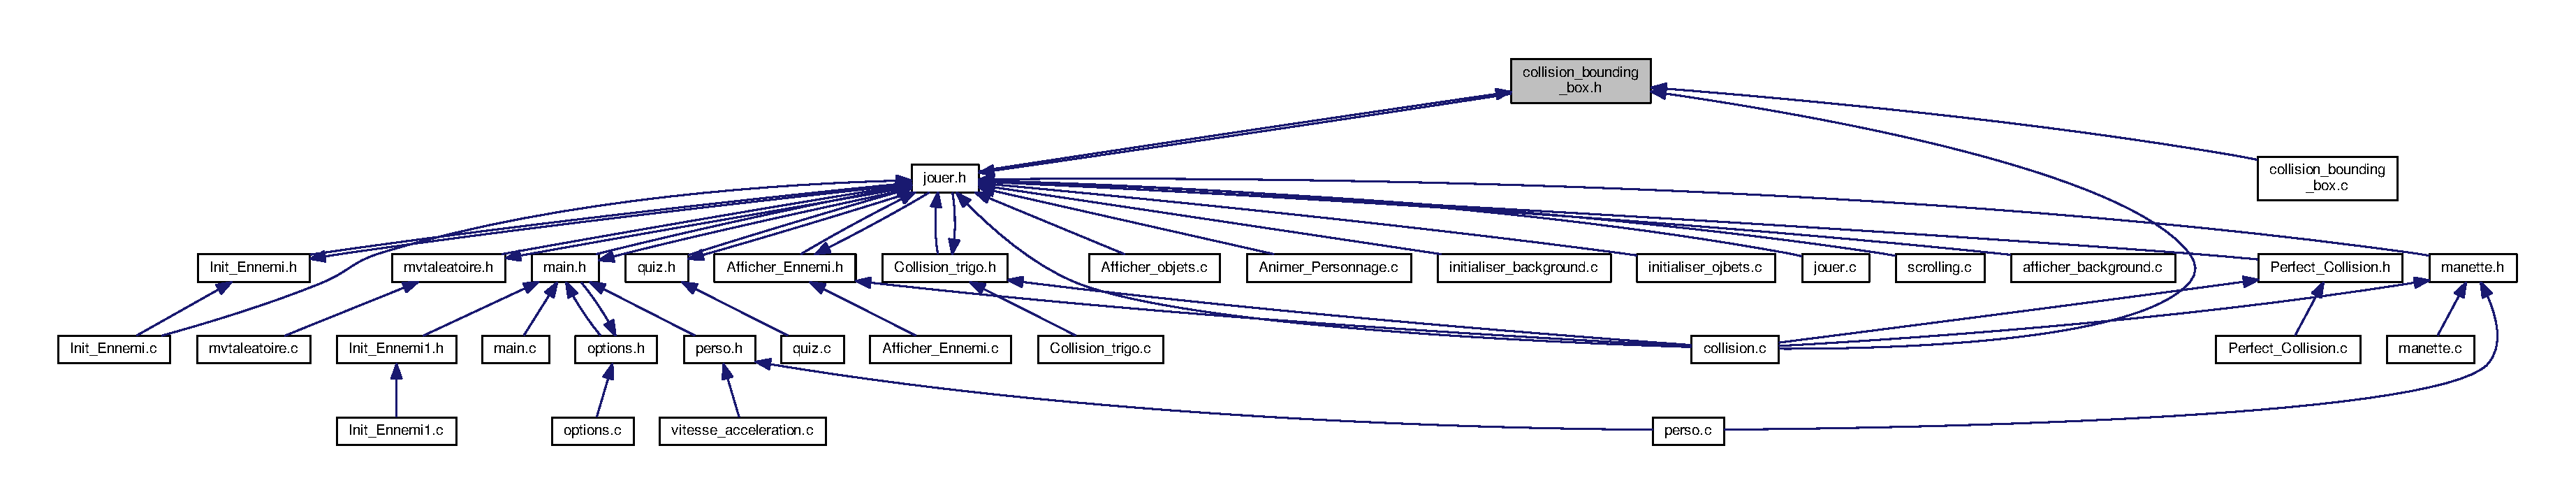
\includegraphics[width=350pt]{collision__bounding__box_8h__dep__incl}
\end{center}
\end{figure}
\subsection*{Functions}
\begin{DoxyCompactItemize}
\item 
int \hyperlink{collision__bounding__box_8h_aaf6f1dec5bb7d4e93d8d580a8e550442}{collision} (S\+D\+L\+\_\+\+Surface $\ast$p, S\+D\+L\+\_\+\+Surface $\ast$e, S\+D\+L\+\_\+\+Rect perso, S\+D\+L\+\_\+\+Rect enemy)
\item 
int \hyperlink{collision__bounding__box_8h_aada0004db077b368ab0b29a7f0e74d72}{collisionbox} (S\+D\+L\+\_\+\+Surface $\ast$p, S\+D\+L\+\_\+\+Surface $\ast$o, S\+D\+L\+\_\+\+Rect perso, S\+D\+L\+\_\+\+Rect objet)
\end{DoxyCompactItemize}


\subsection{Function Documentation}
\index{collision\+\_\+bounding\+\_\+box.\+h@{collision\+\_\+bounding\+\_\+box.\+h}!collision@{collision}}
\index{collision@{collision}!collision\+\_\+bounding\+\_\+box.\+h@{collision\+\_\+bounding\+\_\+box.\+h}}
\subsubsection[{\texorpdfstring{collision(\+S\+D\+L\+\_\+\+Surface $\ast$p, S\+D\+L\+\_\+\+Surface $\ast$e, S\+D\+L\+\_\+\+Rect perso, S\+D\+L\+\_\+\+Rect enemy)}{collision(SDL_Surface *p, SDL_Surface *e, SDL_Rect perso, SDL_Rect enemy)}}]{\setlength{\rightskip}{0pt plus 5cm}int collision (
\begin{DoxyParamCaption}
\item[{S\+D\+L\+\_\+\+Surface $\ast$}]{p, }
\item[{S\+D\+L\+\_\+\+Surface $\ast$}]{e, }
\item[{S\+D\+L\+\_\+\+Rect}]{perso, }
\item[{S\+D\+L\+\_\+\+Rect}]{enemy}
\end{DoxyParamCaption}
)}\hypertarget{collision__bounding__box_8h_aaf6f1dec5bb7d4e93d8d580a8e550442}{}\label{collision__bounding__box_8h_aaf6f1dec5bb7d4e93d8d580a8e550442}
\index{collision\+\_\+bounding\+\_\+box.\+h@{collision\+\_\+bounding\+\_\+box.\+h}!collisionbox@{collisionbox}}
\index{collisionbox@{collisionbox}!collision\+\_\+bounding\+\_\+box.\+h@{collision\+\_\+bounding\+\_\+box.\+h}}
\subsubsection[{\texorpdfstring{collisionbox(\+S\+D\+L\+\_\+\+Surface $\ast$p, S\+D\+L\+\_\+\+Surface $\ast$o, S\+D\+L\+\_\+\+Rect perso, S\+D\+L\+\_\+\+Rect objet)}{collisionbox(SDL_Surface *p, SDL_Surface *o, SDL_Rect perso, SDL_Rect objet)}}]{\setlength{\rightskip}{0pt plus 5cm}int collisionbox (
\begin{DoxyParamCaption}
\item[{S\+D\+L\+\_\+\+Surface $\ast$}]{p, }
\item[{S\+D\+L\+\_\+\+Surface $\ast$}]{o, }
\item[{S\+D\+L\+\_\+\+Rect}]{perso, }
\item[{S\+D\+L\+\_\+\+Rect}]{objet}
\end{DoxyParamCaption}
)}\hypertarget{collision__bounding__box_8h_aada0004db077b368ab0b29a7f0e74d72}{}\label{collision__bounding__box_8h_aada0004db077b368ab0b29a7f0e74d72}

\hypertarget{Collision__trigo_8c}{}\section{Collision\+\_\+trigo.\+c File Reference}
\label{Collision__trigo_8c}\index{Collision\+\_\+trigo.\+c@{Collision\+\_\+trigo.\+c}}
{\ttfamily \#include $<$stdlib.\+h$>$}\\*
{\ttfamily \#include $<$stdio.\+h$>$}\\*
{\ttfamily \#include $<$S\+D\+L/\+S\+D\+L.\+h$>$}\\*
{\ttfamily \#include \char`\"{}Collision\+\_\+trigo.\+h\char`\"{}}\\*
Include dependency graph for Collision\+\_\+trigo.\+c\+:
\nopagebreak
\begin{figure}[H]
\begin{center}
\leavevmode
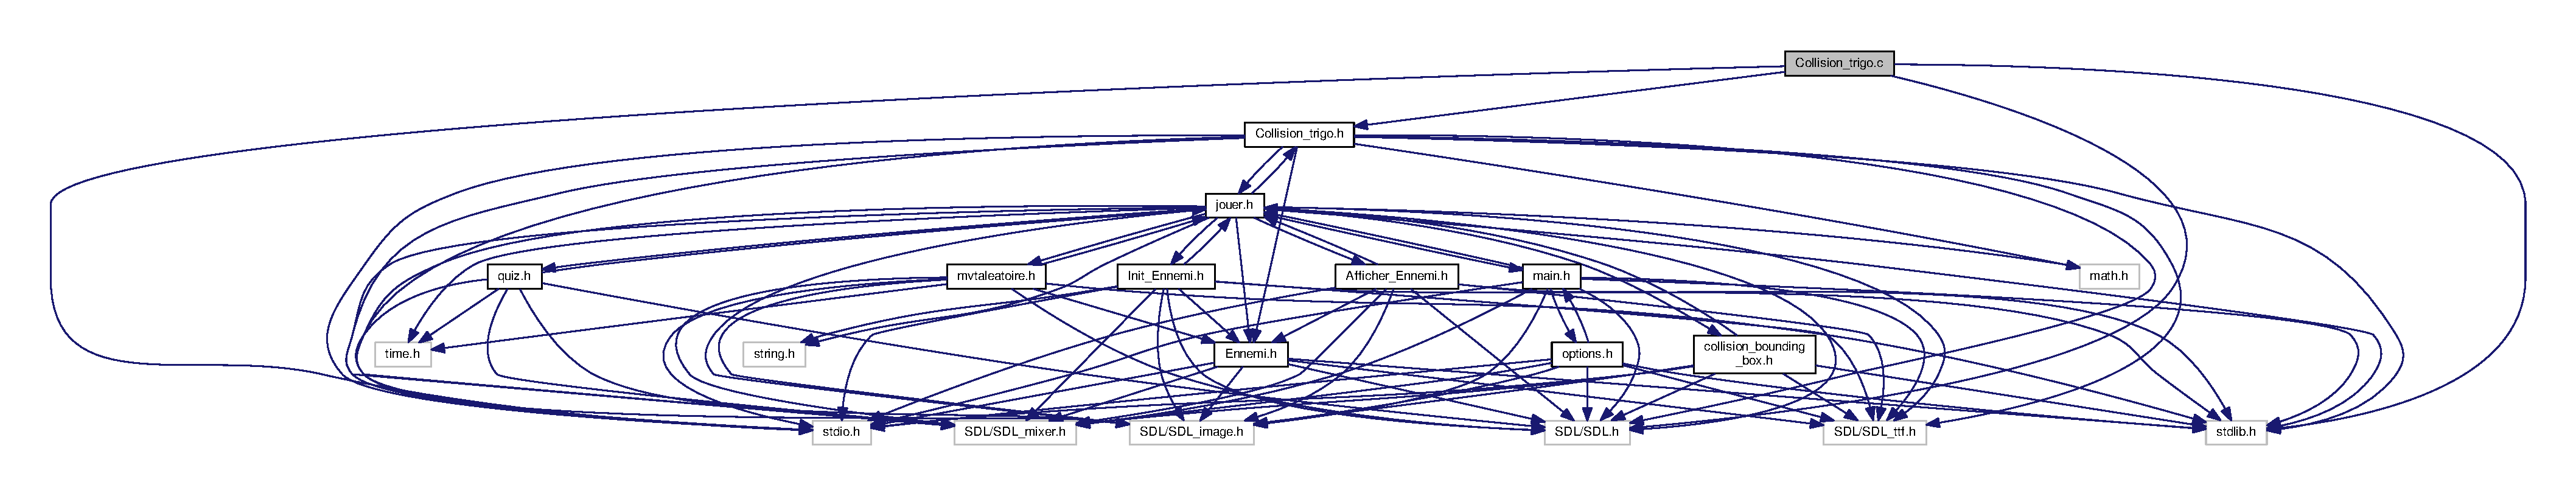
\includegraphics[width=350pt]{Collision__trigo_8c__incl}
\end{center}
\end{figure}
\subsection*{Functions}
\begin{DoxyCompactItemize}
\item 
int \hyperlink{Collision__trigo_8c_aa7a006f89e162da81cf20be078bf3653}{Collision\+\_\+\+Ennemi} (S\+D\+L\+\_\+\+Rect Pos\+\_\+perso, \hyperlink{structEnnemi}{Ennemi} Mob)
\end{DoxyCompactItemize}


\subsection{Function Documentation}
\index{Collision\+\_\+trigo.\+c@{Collision\+\_\+trigo.\+c}!Collision\+\_\+\+Ennemi@{Collision\+\_\+\+Ennemi}}
\index{Collision\+\_\+\+Ennemi@{Collision\+\_\+\+Ennemi}!Collision\+\_\+trigo.\+c@{Collision\+\_\+trigo.\+c}}
\subsubsection[{\texorpdfstring{Collision\+\_\+\+Ennemi(\+S\+D\+L\+\_\+\+Rect Pos\+\_\+perso, Ennemi Mob)}{Collision_Ennemi(SDL_Rect Pos_perso, Ennemi Mob)}}]{\setlength{\rightskip}{0pt plus 5cm}int Collision\+\_\+\+Ennemi (
\begin{DoxyParamCaption}
\item[{S\+D\+L\+\_\+\+Rect}]{Pos\+\_\+perso, }
\item[{{\bf Ennemi}}]{Mob}
\end{DoxyParamCaption}
)}\hypertarget{Collision__trigo_8c_aa7a006f89e162da81cf20be078bf3653}{}\label{Collision__trigo_8c_aa7a006f89e162da81cf20be078bf3653}


Here is the call graph for this function\+:\nopagebreak
\begin{figure}[H]
\begin{center}
\leavevmode
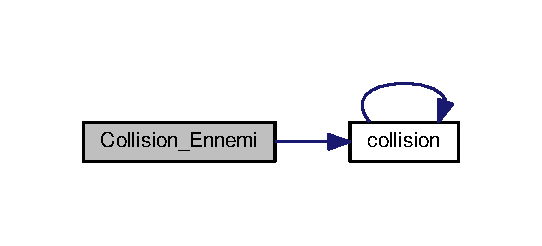
\includegraphics[width=260pt]{Collision__trigo_8c_aa7a006f89e162da81cf20be078bf3653_cgraph}
\end{center}
\end{figure}




Here is the caller graph for this function\+:
\nopagebreak
\begin{figure}[H]
\begin{center}
\leavevmode
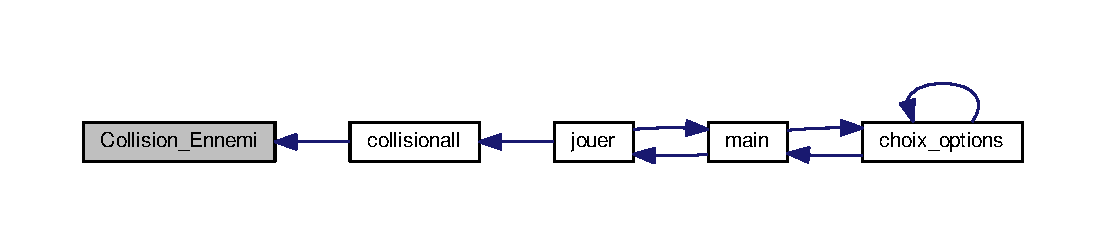
\includegraphics[width=350pt]{Collision__trigo_8c_aa7a006f89e162da81cf20be078bf3653_icgraph}
\end{center}
\end{figure}



\hypertarget{Collision__trigo_8h}{}\section{Collision\+\_\+trigo.\+h File Reference}
\label{Collision__trigo_8h}\index{Collision\+\_\+trigo.\+h@{Collision\+\_\+trigo.\+h}}
{\ttfamily \#include $<$stdlib.\+h$>$}\\*
{\ttfamily \#include $<$stdio.\+h$>$}\\*
{\ttfamily \#include $<$math.\+h$>$}\\*
{\ttfamily \#include $<$S\+D\+L/\+S\+D\+L.\+h$>$}\\*
{\ttfamily \#include $<$S\+D\+L/\+S\+D\+L\+\_\+image.\+h$>$}\\*
{\ttfamily \#include $<$S\+D\+L/\+S\+D\+L\+\_\+mixer.\+h$>$}\\*
{\ttfamily \#include $<$S\+D\+L/\+S\+D\+L\+\_\+ttf.\+h$>$}\\*
{\ttfamily \#include \char`\"{}Ennemi.\+h\char`\"{}}\\*
{\ttfamily \#include \char`\"{}jouer.\+h\char`\"{}}\\*
Include dependency graph for Collision\+\_\+trigo.\+h\+:
\nopagebreak
\begin{figure}[H]
\begin{center}
\leavevmode
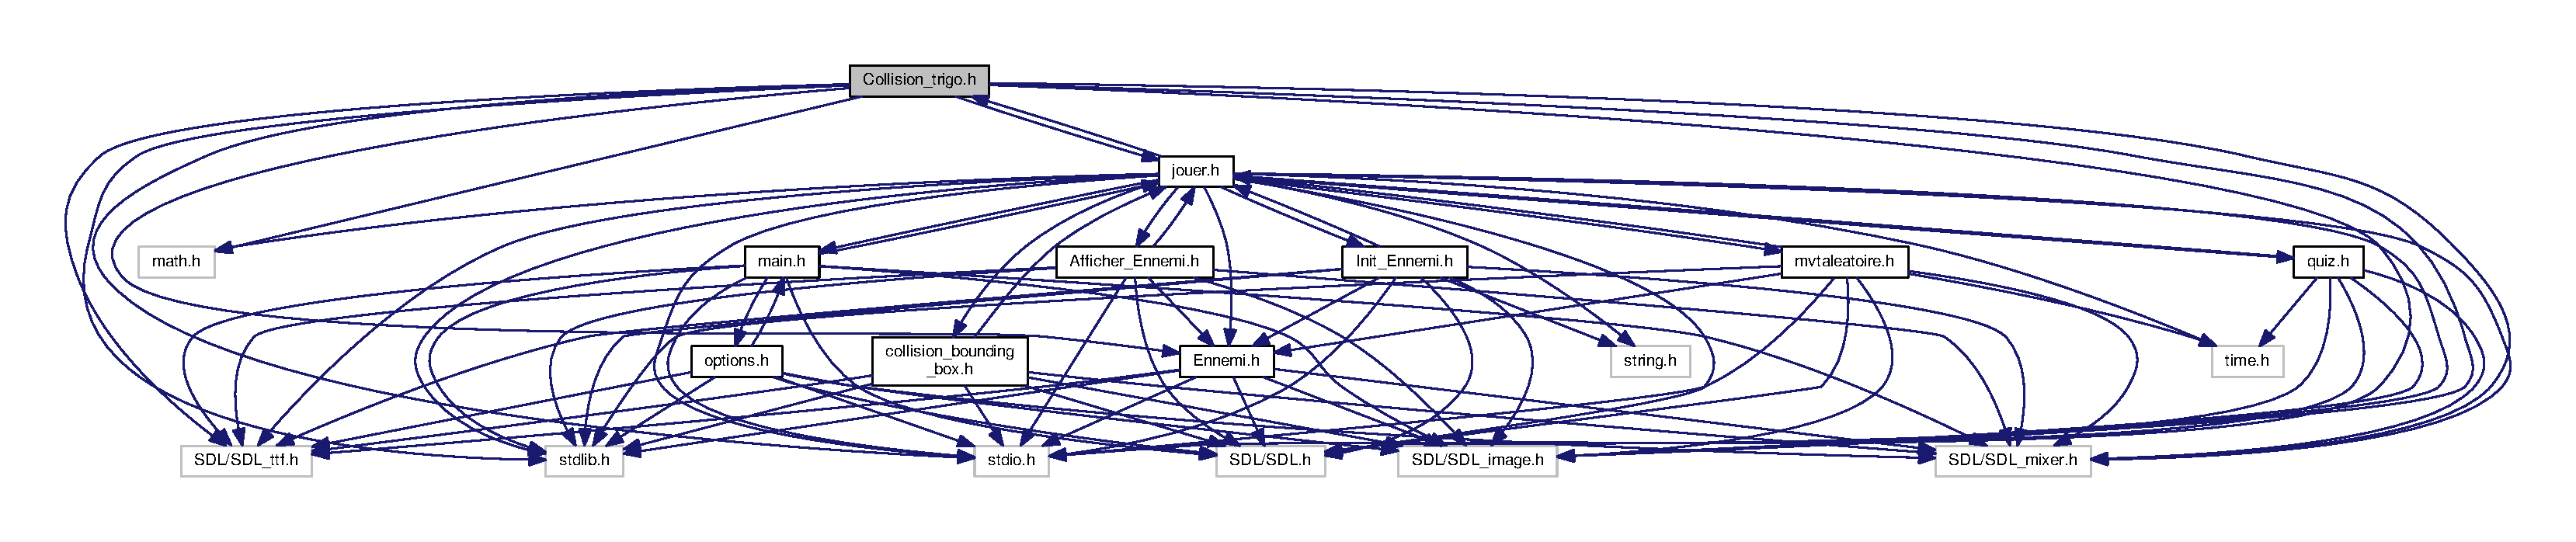
\includegraphics[width=350pt]{Collision__trigo_8h__incl}
\end{center}
\end{figure}
This graph shows which files directly or indirectly include this file\+:
\nopagebreak
\begin{figure}[H]
\begin{center}
\leavevmode
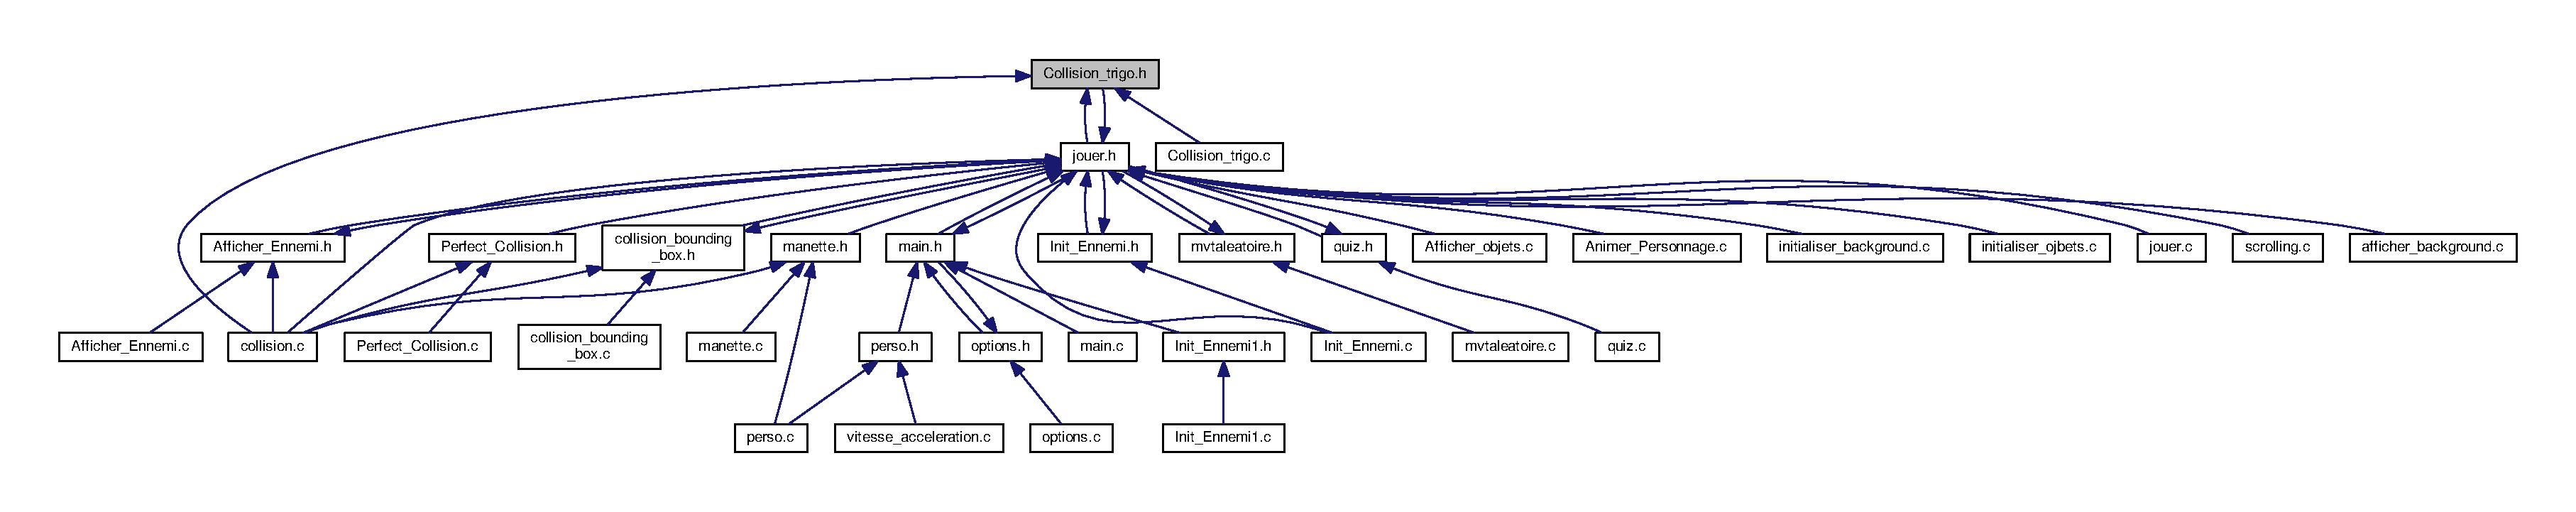
\includegraphics[width=350pt]{Collision__trigo_8h__dep__incl}
\end{center}
\end{figure}
\subsection*{Functions}
\begin{DoxyCompactItemize}
\item 
int \hyperlink{Collision__trigo_8h_aa7a006f89e162da81cf20be078bf3653}{Collision\+\_\+\+Ennemi} (S\+D\+L\+\_\+\+Rect Pos\+\_\+perso, \hyperlink{structEnnemi}{Ennemi} Mob)
\end{DoxyCompactItemize}


\subsection{Function Documentation}
\index{Collision\+\_\+trigo.\+h@{Collision\+\_\+trigo.\+h}!Collision\+\_\+\+Ennemi@{Collision\+\_\+\+Ennemi}}
\index{Collision\+\_\+\+Ennemi@{Collision\+\_\+\+Ennemi}!Collision\+\_\+trigo.\+h@{Collision\+\_\+trigo.\+h}}
\subsubsection[{\texorpdfstring{Collision\+\_\+\+Ennemi(\+S\+D\+L\+\_\+\+Rect Pos\+\_\+perso, Ennemi Mob)}{Collision_Ennemi(SDL_Rect Pos_perso, Ennemi Mob)}}]{\setlength{\rightskip}{0pt plus 5cm}int Collision\+\_\+\+Ennemi (
\begin{DoxyParamCaption}
\item[{S\+D\+L\+\_\+\+Rect}]{Pos\+\_\+perso, }
\item[{{\bf Ennemi}}]{Mob}
\end{DoxyParamCaption}
)}\hypertarget{Collision__trigo_8h_aa7a006f89e162da81cf20be078bf3653}{}\label{Collision__trigo_8h_aa7a006f89e162da81cf20be078bf3653}

\hypertarget{Defs_8h}{}\section{Defs.\+h File Reference}
\label{Defs_8h}\index{Defs.\+h@{Defs.\+h}}
{\ttfamily \#include $<$stdlib.\+h$>$}\\*
{\ttfamily \#include $<$stdio.\+h$>$}\\*
{\ttfamily \#include $<$S\+D\+L/\+S\+D\+L.\+h$>$}\\*
{\ttfamily \#include $<$S\+D\+L/\+S\+D\+L\+\_\+mixer.\+h$>$}\\*
{\ttfamily \#include $<$S\+D\+L/\+S\+D\+L\+\_\+ttf.\+h$>$}\\*
Include dependency graph for Defs.\+h\+:
\nopagebreak
\begin{figure}[H]
\begin{center}
\leavevmode
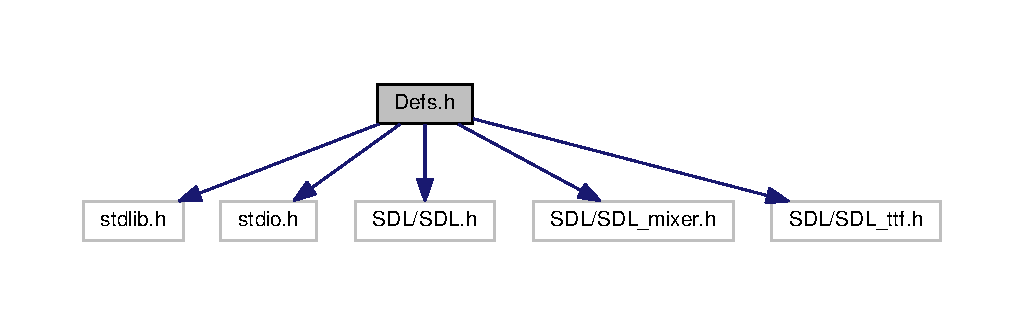
\includegraphics[width=350pt]{Defs_8h__incl}
\end{center}
\end{figure}

\hypertarget{Ennemi_8h}{}\section{Ennemi.\+h File Reference}
\label{Ennemi_8h}\index{Ennemi.\+h@{Ennemi.\+h}}
{\ttfamily \#include $<$stdlib.\+h$>$}\\*
{\ttfamily \#include $<$stdio.\+h$>$}\\*
{\ttfamily \#include $<$S\+D\+L/\+S\+D\+L.\+h$>$}\\*
{\ttfamily \#include $<$S\+D\+L/\+S\+D\+L\+\_\+image.\+h$>$}\\*
{\ttfamily \#include $<$S\+D\+L/\+S\+D\+L\+\_\+mixer.\+h$>$}\\*
{\ttfamily \#include $<$S\+D\+L/\+S\+D\+L\+\_\+ttf.\+h$>$}\\*
Include dependency graph for Ennemi.\+h\+:\nopagebreak
\begin{figure}[H]
\begin{center}
\leavevmode
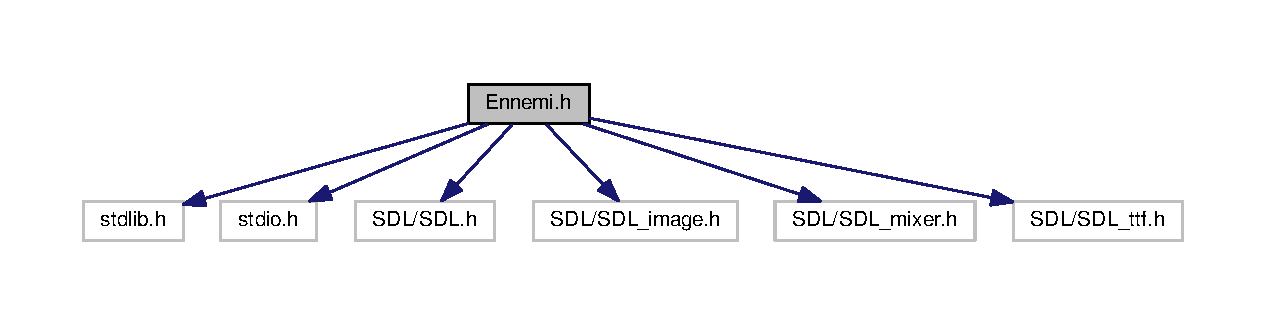
\includegraphics[width=350pt]{Ennemi_8h__incl}
\end{center}
\end{figure}
This graph shows which files directly or indirectly include this file\+:
\nopagebreak
\begin{figure}[H]
\begin{center}
\leavevmode
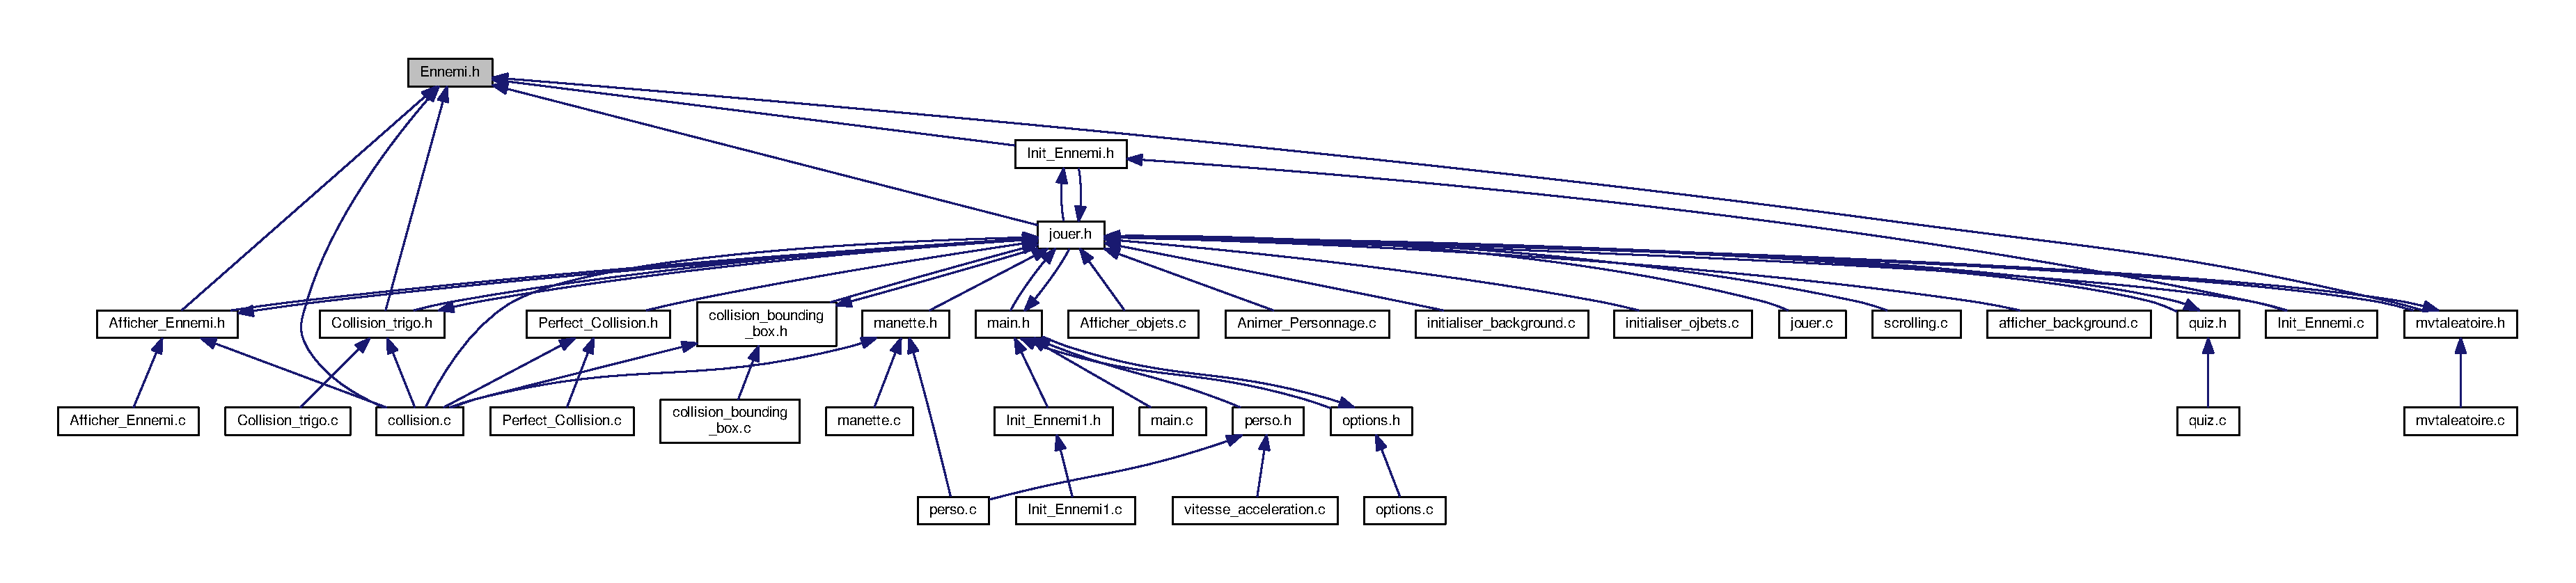
\includegraphics[width=350pt]{Ennemi_8h__dep__incl}
\end{center}
\end{figure}
\subsection*{Classes}
\begin{DoxyCompactItemize}
\item 
struct \hyperlink{structEnnemi}{Ennemi}
\end{DoxyCompactItemize}

\hypertarget{Init__Ennemi_8c}{}\section{Init\+\_\+\+Ennemi.\+c File Reference}
\label{Init__Ennemi_8c}\index{Init\+\_\+\+Ennemi.\+c@{Init\+\_\+\+Ennemi.\+c}}
{\ttfamily \#include $<$stdlib.\+h$>$}\\*
{\ttfamily \#include $<$stdio.\+h$>$}\\*
{\ttfamily \#include $<$S\+D\+L/\+S\+D\+L.\+h$>$}\\*
{\ttfamily \#include \char`\"{}Init\+\_\+\+Ennemi.\+h\char`\"{}}\\*
{\ttfamily \#include \char`\"{}jouer.\+h\char`\"{}}\\*
Include dependency graph for Init\+\_\+\+Ennemi.\+c\+:
\nopagebreak
\begin{figure}[H]
\begin{center}
\leavevmode
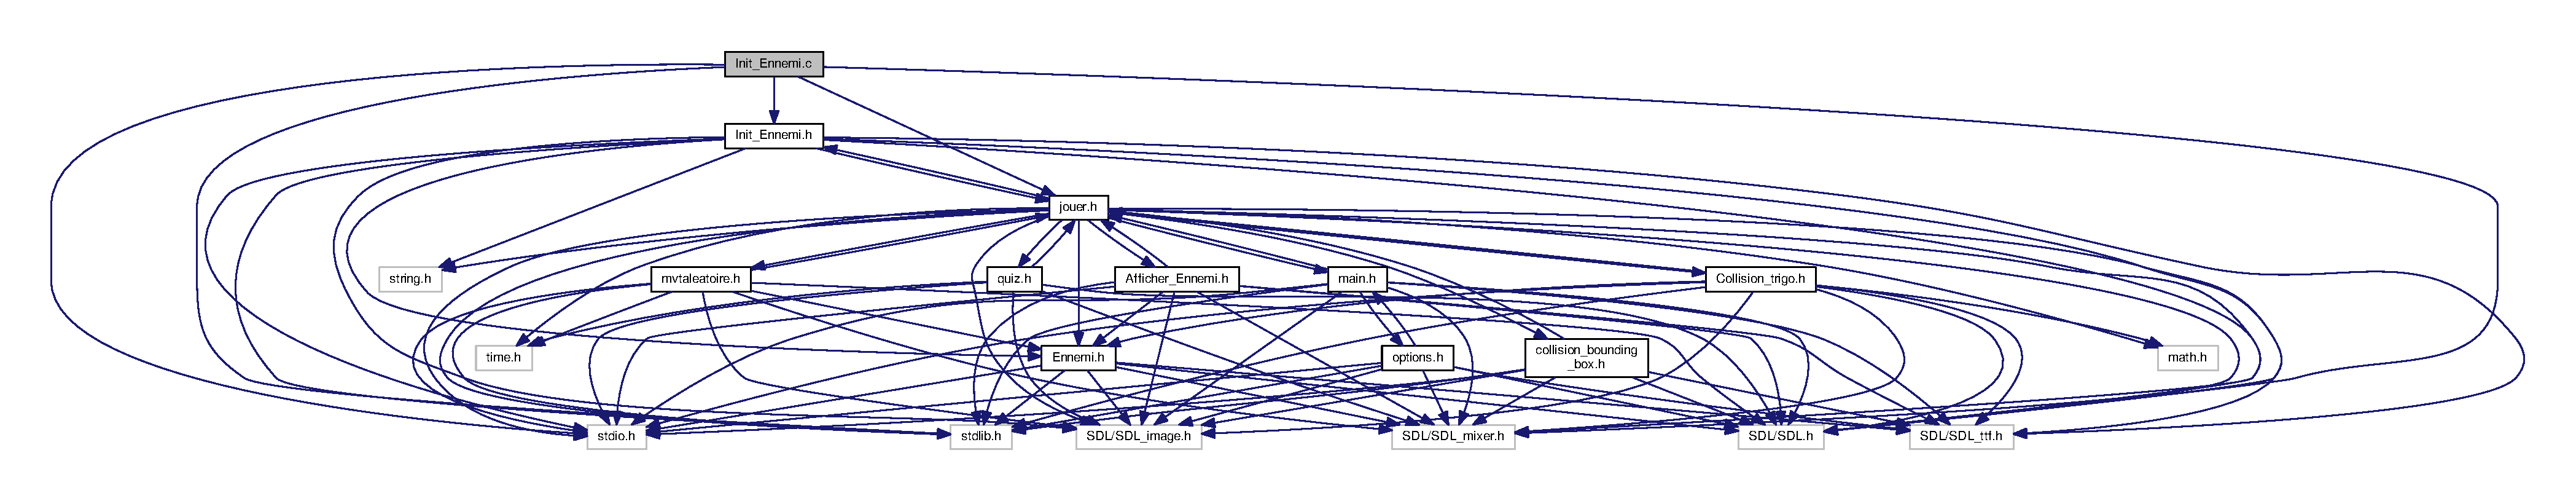
\includegraphics[width=350pt]{Init__Ennemi_8c__incl}
\end{center}
\end{figure}
\subsection*{Functions}
\begin{DoxyCompactItemize}
\item 
\hyperlink{structEnnemi}{Ennemi} \hyperlink{Init__Ennemi_8c_acc0a5eae1c2488e30bf55a4b064cc833}{Init\+\_\+\+Ennemi} (char Mob\+\_\+\+Name\mbox{[}$\,$\mbox{]}, int X, int Y)
\end{DoxyCompactItemize}


\subsection{Function Documentation}
\index{Init\+\_\+\+Ennemi.\+c@{Init\+\_\+\+Ennemi.\+c}!Init\+\_\+\+Ennemi@{Init\+\_\+\+Ennemi}}
\index{Init\+\_\+\+Ennemi@{Init\+\_\+\+Ennemi}!Init\+\_\+\+Ennemi.\+c@{Init\+\_\+\+Ennemi.\+c}}
\subsubsection[{\texorpdfstring{Init\+\_\+\+Ennemi(char Mob\+\_\+\+Name[], int X, int Y)}{Init_Ennemi(char Mob_Name[], int X, int Y)}}]{\setlength{\rightskip}{0pt plus 5cm}{\bf Ennemi} Init\+\_\+\+Ennemi (
\begin{DoxyParamCaption}
\item[{char}]{Mob\+\_\+\+Name\mbox{[}$\,$\mbox{]}, }
\item[{int}]{X, }
\item[{int}]{Y}
\end{DoxyParamCaption}
)}\hypertarget{Init__Ennemi_8c_acc0a5eae1c2488e30bf55a4b064cc833}{}\label{Init__Ennemi_8c_acc0a5eae1c2488e30bf55a4b064cc833}


Here is the caller graph for this function\+:
\nopagebreak
\begin{figure}[H]
\begin{center}
\leavevmode
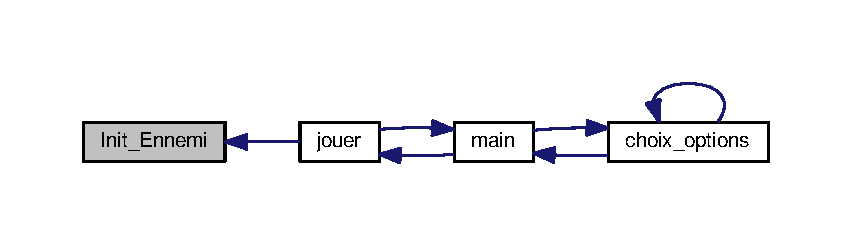
\includegraphics[width=350pt]{Init__Ennemi_8c_acc0a5eae1c2488e30bf55a4b064cc833_icgraph}
\end{center}
\end{figure}



\hypertarget{Init__Ennemi_8h}{}\section{Init\+\_\+\+Ennemi.\+h File Reference}
\label{Init__Ennemi_8h}\index{Init\+\_\+\+Ennemi.\+h@{Init\+\_\+\+Ennemi.\+h}}
{\ttfamily \#include $<$stdlib.\+h$>$}\\*
{\ttfamily \#include $<$stdio.\+h$>$}\\*
{\ttfamily \#include $<$S\+D\+L/\+S\+D\+L.\+h$>$}\\*
{\ttfamily \#include $<$string.\+h$>$}\\*
{\ttfamily \#include $<$S\+D\+L/\+S\+D\+L\+\_\+image.\+h$>$}\\*
{\ttfamily \#include $<$S\+D\+L/\+S\+D\+L\+\_\+mixer.\+h$>$}\\*
{\ttfamily \#include $<$S\+D\+L/\+S\+D\+L\+\_\+ttf.\+h$>$}\\*
{\ttfamily \#include \char`\"{}Ennemi.\+h\char`\"{}}\\*
{\ttfamily \#include \char`\"{}jouer.\+h\char`\"{}}\\*
Include dependency graph for Init\+\_\+\+Ennemi.\+h\+:
\nopagebreak
\begin{figure}[H]
\begin{center}
\leavevmode
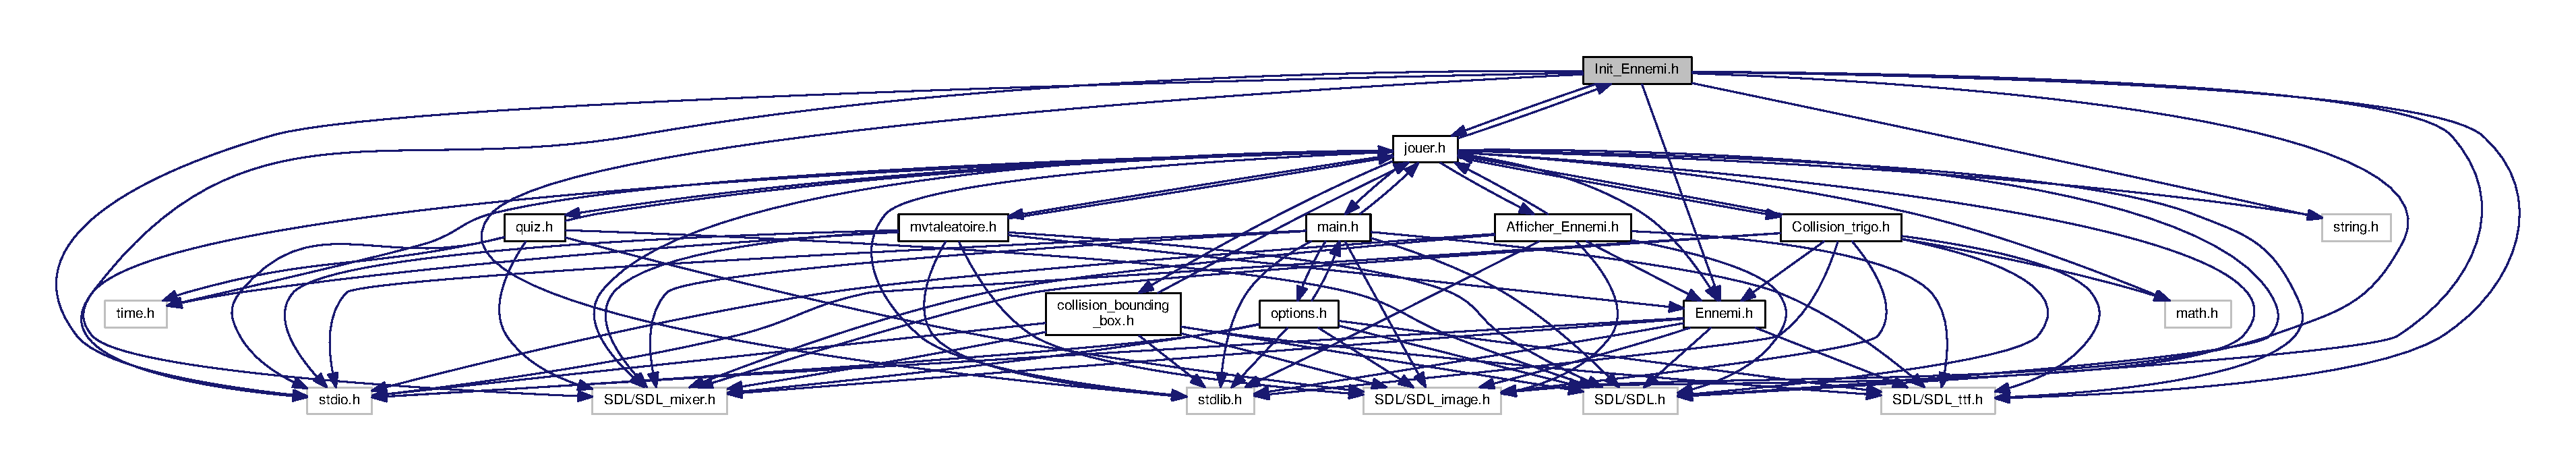
\includegraphics[width=350pt]{Init__Ennemi_8h__incl}
\end{center}
\end{figure}
This graph shows which files directly or indirectly include this file\+:
\nopagebreak
\begin{figure}[H]
\begin{center}
\leavevmode
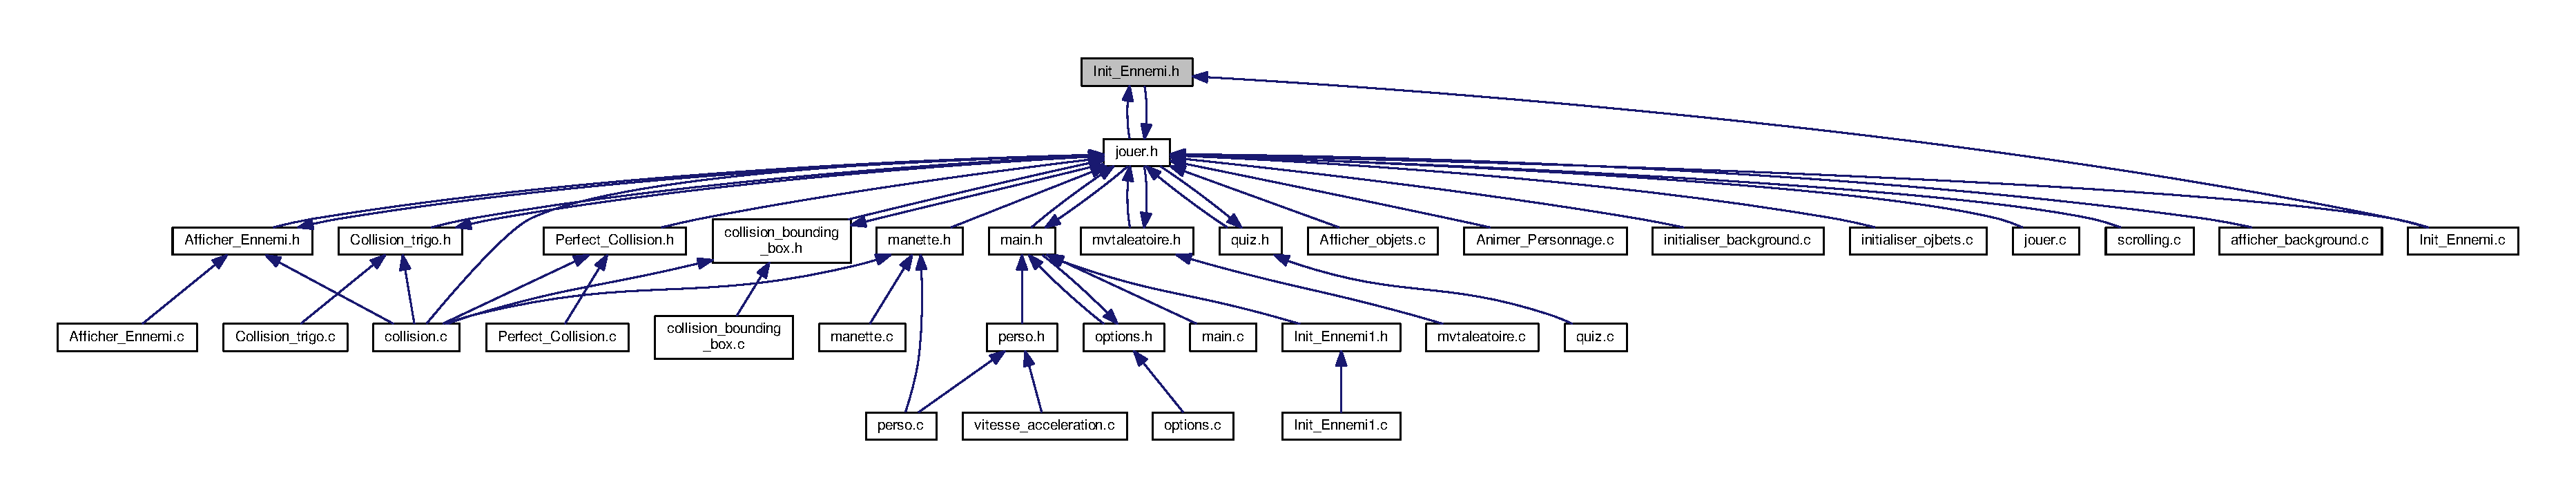
\includegraphics[width=350pt]{Init__Ennemi_8h__dep__incl}
\end{center}
\end{figure}
\subsection*{Functions}
\begin{DoxyCompactItemize}
\item 
\hyperlink{structEnnemi}{Ennemi} \hyperlink{Init__Ennemi_8h_acc0a5eae1c2488e30bf55a4b064cc833}{Init\+\_\+\+Ennemi} (char Mob\+\_\+\+Name\mbox{[}$\,$\mbox{]}, int X, int Y)
\end{DoxyCompactItemize}


\subsection{Function Documentation}
\index{Init\+\_\+\+Ennemi.\+h@{Init\+\_\+\+Ennemi.\+h}!Init\+\_\+\+Ennemi@{Init\+\_\+\+Ennemi}}
\index{Init\+\_\+\+Ennemi@{Init\+\_\+\+Ennemi}!Init\+\_\+\+Ennemi.\+h@{Init\+\_\+\+Ennemi.\+h}}
\subsubsection[{\texorpdfstring{Init\+\_\+\+Ennemi(char Mob\+\_\+\+Name[], int X, int Y)}{Init_Ennemi(char Mob_Name[], int X, int Y)}}]{\setlength{\rightskip}{0pt plus 5cm}{\bf Ennemi} Init\+\_\+\+Ennemi (
\begin{DoxyParamCaption}
\item[{char}]{Mob\+\_\+\+Name\mbox{[}$\,$\mbox{]}, }
\item[{int}]{X, }
\item[{int}]{Y}
\end{DoxyParamCaption}
)}\hypertarget{Init__Ennemi_8h_acc0a5eae1c2488e30bf55a4b064cc833}{}\label{Init__Ennemi_8h_acc0a5eae1c2488e30bf55a4b064cc833}

\hypertarget{Init__Ennemi1_8c}{}\section{Init\+\_\+\+Ennemi1.\+c File Reference}
\label{Init__Ennemi1_8c}\index{Init\+\_\+\+Ennemi1.\+c@{Init\+\_\+\+Ennemi1.\+c}}
{\ttfamily \#include $<$stdlib.\+h$>$}\\*
{\ttfamily \#include $<$stdio.\+h$>$}\\*
{\ttfamily \#include $<$S\+D\+L/\+S\+D\+L.\+h$>$}\\*
{\ttfamily \#include \char`\"{}Init\+\_\+\+Ennemi1.\+h\char`\"{}}\\*
Include dependency graph for Init\+\_\+\+Ennemi1.\+c\+:
\nopagebreak
\begin{figure}[H]
\begin{center}
\leavevmode
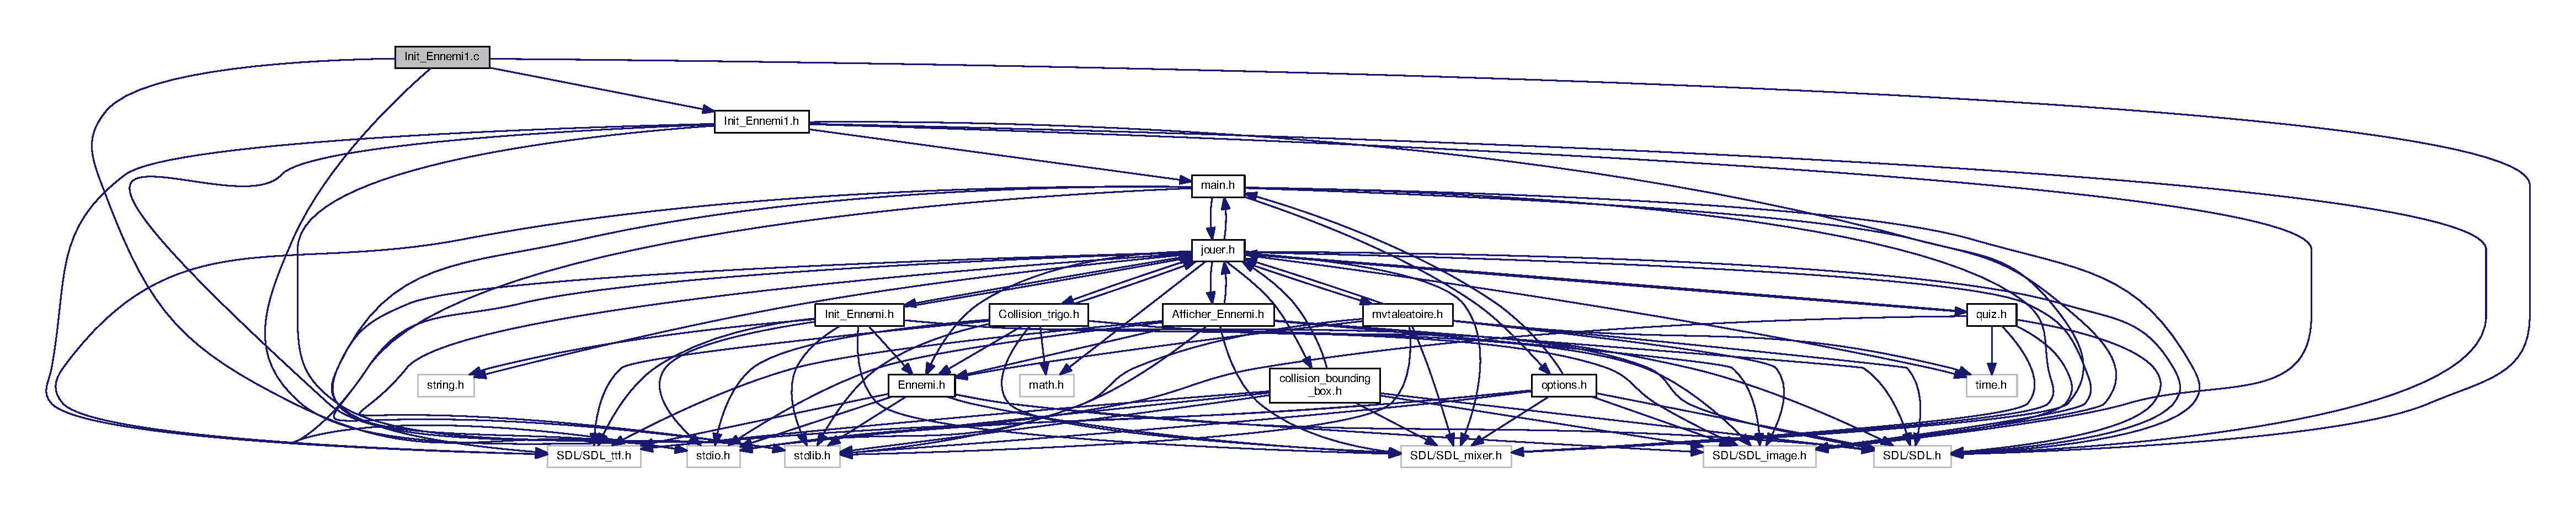
\includegraphics[width=350pt]{Init__Ennemi1_8c__incl}
\end{center}
\end{figure}
\subsection*{Functions}
\begin{DoxyCompactItemize}
\item 
\hyperlink{structEnnemii}{Ennemii} \hyperlink{Init__Ennemi1_8c_a21ded47b333fb3f6a0dd9105ec8e0209}{Init\+\_\+\+Ennemi1} ()
\end{DoxyCompactItemize}


\subsection{Function Documentation}
\index{Init\+\_\+\+Ennemi1.\+c@{Init\+\_\+\+Ennemi1.\+c}!Init\+\_\+\+Ennemi1@{Init\+\_\+\+Ennemi1}}
\index{Init\+\_\+\+Ennemi1@{Init\+\_\+\+Ennemi1}!Init\+\_\+\+Ennemi1.\+c@{Init\+\_\+\+Ennemi1.\+c}}
\subsubsection[{\texorpdfstring{Init\+\_\+\+Ennemi1()}{Init_Ennemi1()}}]{\setlength{\rightskip}{0pt plus 5cm}{\bf Ennemii} Init\+\_\+\+Ennemi1 (
\begin{DoxyParamCaption}
{}
\end{DoxyParamCaption}
)}\hypertarget{Init__Ennemi1_8c_a21ded47b333fb3f6a0dd9105ec8e0209}{}\label{Init__Ennemi1_8c_a21ded47b333fb3f6a0dd9105ec8e0209}


Here is the caller graph for this function\+:
\nopagebreak
\begin{figure}[H]
\begin{center}
\leavevmode
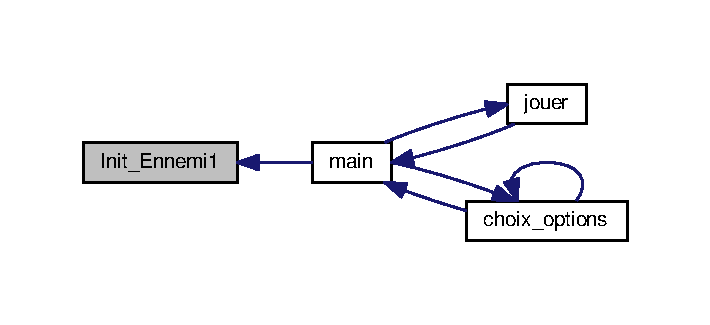
\includegraphics[width=341pt]{Init__Ennemi1_8c_a21ded47b333fb3f6a0dd9105ec8e0209_icgraph}
\end{center}
\end{figure}



\hypertarget{Init__Ennemi1_8h}{}\section{Init\+\_\+\+Ennemi1.\+h File Reference}
\label{Init__Ennemi1_8h}\index{Init\+\_\+\+Ennemi1.\+h@{Init\+\_\+\+Ennemi1.\+h}}
{\ttfamily \#include $<$stdlib.\+h$>$}\\*
{\ttfamily \#include $<$stdio.\+h$>$}\\*
{\ttfamily \#include $<$S\+D\+L/\+S\+D\+L.\+h$>$}\\*
{\ttfamily \#include $<$S\+D\+L/\+S\+D\+L\+\_\+image.\+h$>$}\\*
{\ttfamily \#include $<$S\+D\+L/\+S\+D\+L\+\_\+mixer.\+h$>$}\\*
{\ttfamily \#include $<$S\+D\+L/\+S\+D\+L\+\_\+ttf.\+h$>$}\\*
{\ttfamily \#include \char`\"{}main.\+h\char`\"{}}\\*
Include dependency graph for Init\+\_\+\+Ennemi1.\+h\+:
\nopagebreak
\begin{figure}[H]
\begin{center}
\leavevmode
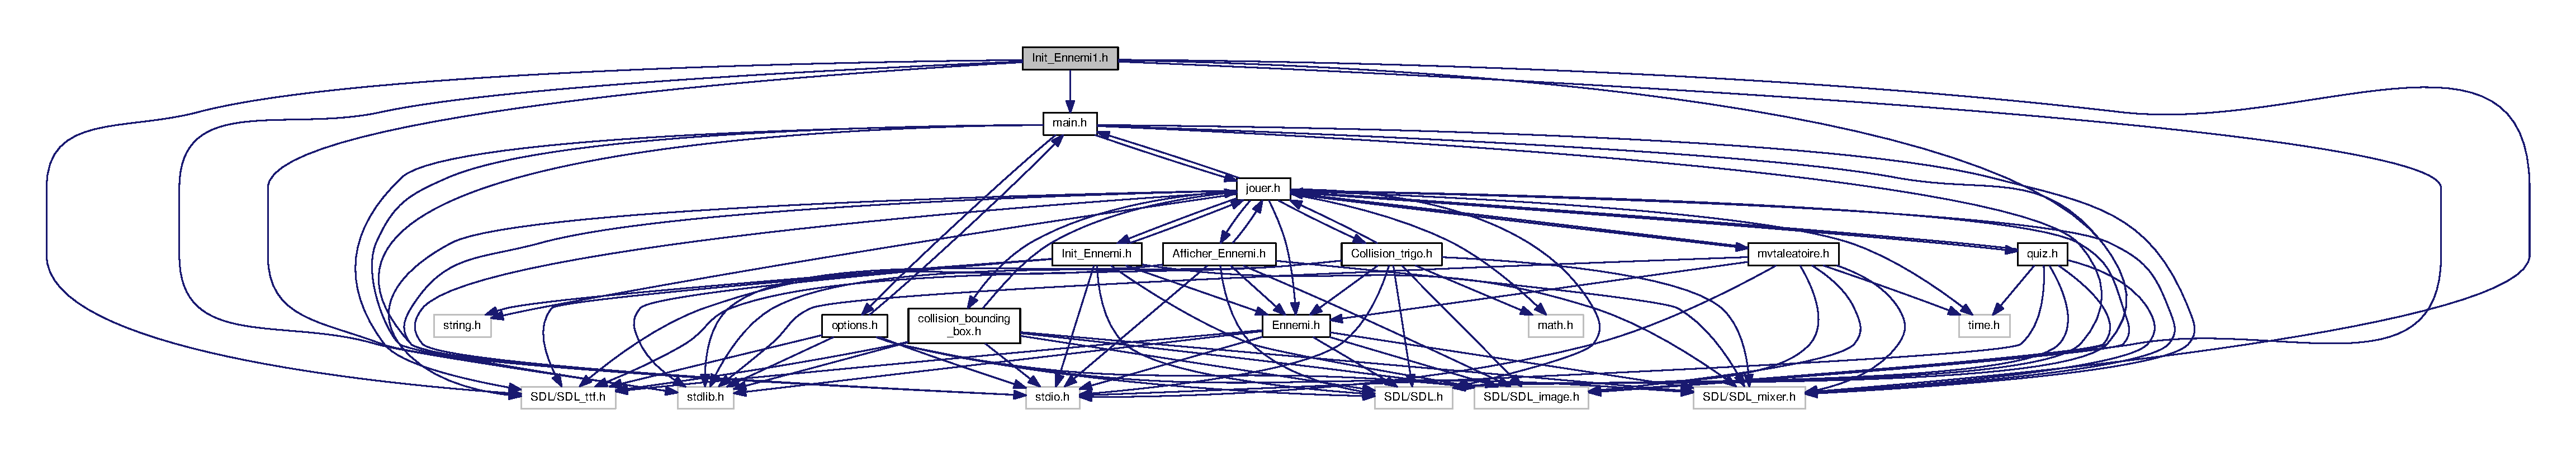
\includegraphics[width=350pt]{Init__Ennemi1_8h__incl}
\end{center}
\end{figure}
This graph shows which files directly or indirectly include this file\+:
\nopagebreak
\begin{figure}[H]
\begin{center}
\leavevmode
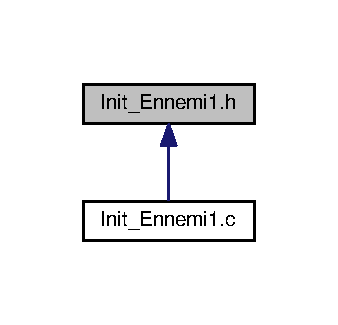
\includegraphics[width=162pt]{Init__Ennemi1_8h__dep__incl}
\end{center}
\end{figure}
\subsection*{Functions}
\begin{DoxyCompactItemize}
\item 
\hyperlink{structEnnemii}{Ennemii} \hyperlink{Init__Ennemi1_8h_a21ded47b333fb3f6a0dd9105ec8e0209}{Init\+\_\+\+Ennemi1} ()
\end{DoxyCompactItemize}


\subsection{Function Documentation}
\index{Init\+\_\+\+Ennemi1.\+h@{Init\+\_\+\+Ennemi1.\+h}!Init\+\_\+\+Ennemi1@{Init\+\_\+\+Ennemi1}}
\index{Init\+\_\+\+Ennemi1@{Init\+\_\+\+Ennemi1}!Init\+\_\+\+Ennemi1.\+h@{Init\+\_\+\+Ennemi1.\+h}}
\subsubsection[{\texorpdfstring{Init\+\_\+\+Ennemi1()}{Init_Ennemi1()}}]{\setlength{\rightskip}{0pt plus 5cm}{\bf Ennemii} Init\+\_\+\+Ennemi1 (
\begin{DoxyParamCaption}
{}
\end{DoxyParamCaption}
)}\hypertarget{Init__Ennemi1_8h_a21ded47b333fb3f6a0dd9105ec8e0209}{}\label{Init__Ennemi1_8h_a21ded47b333fb3f6a0dd9105ec8e0209}

\hypertarget{initialiser__background_8c}{}\section{initialiser\+\_\+background.\+c File Reference}
\label{initialiser__background_8c}\index{initialiser\+\_\+background.\+c@{initialiser\+\_\+background.\+c}}
{\ttfamily \#include $<$stdlib.\+h$>$}\\*
{\ttfamily \#include $<$stdio.\+h$>$}\\*
{\ttfamily \#include $<$S\+D\+L/\+S\+D\+L.\+h$>$}\\*
{\ttfamily \#include \char`\"{}jouer.\+h\char`\"{}}\\*
Include dependency graph for initialiser\+\_\+background.\+c\+:
\nopagebreak
\begin{figure}[H]
\begin{center}
\leavevmode
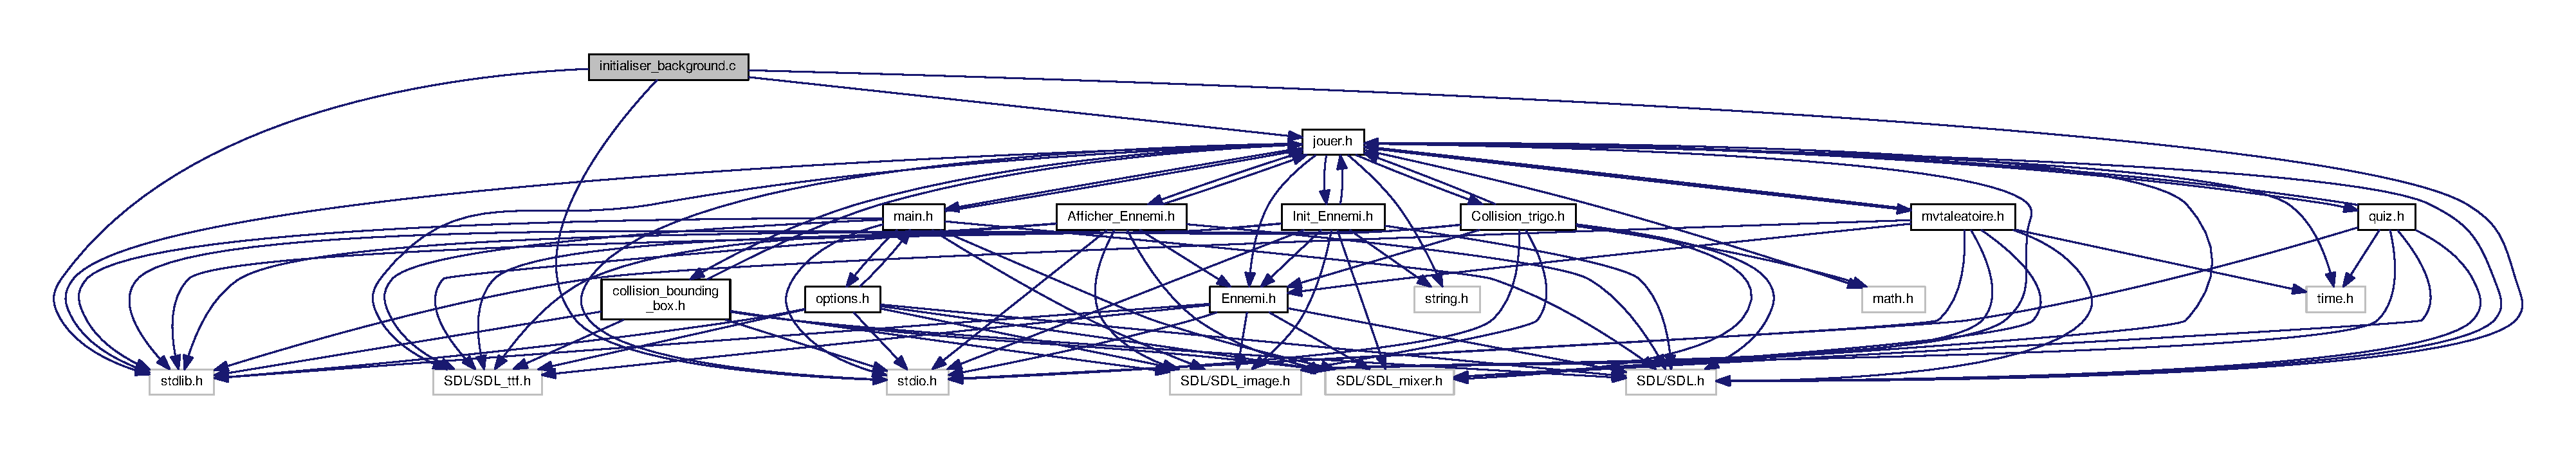
\includegraphics[width=350pt]{initialiser__background_8c__incl}
\end{center}
\end{figure}
\subsection*{Functions}
\begin{DoxyCompactItemize}
\item 
void \hyperlink{initialiser__background_8c_a627e8dbcc77f69a29241e6dccf38d77d}{initialiser} (\hyperlink{structbackground}{background} $\ast$b)
\end{DoxyCompactItemize}


\subsection{Function Documentation}
\index{initialiser\+\_\+background.\+c@{initialiser\+\_\+background.\+c}!initialiser@{initialiser}}
\index{initialiser@{initialiser}!initialiser\+\_\+background.\+c@{initialiser\+\_\+background.\+c}}
\subsubsection[{\texorpdfstring{initialiser(background $\ast$b)}{initialiser(background *b)}}]{\setlength{\rightskip}{0pt plus 5cm}void initialiser (
\begin{DoxyParamCaption}
\item[{{\bf background} $\ast$}]{b}
\end{DoxyParamCaption}
)}\hypertarget{initialiser__background_8c_a627e8dbcc77f69a29241e6dccf38d77d}{}\label{initialiser__background_8c_a627e8dbcc77f69a29241e6dccf38d77d}


Here is the caller graph for this function\+:
\nopagebreak
\begin{figure}[H]
\begin{center}
\leavevmode
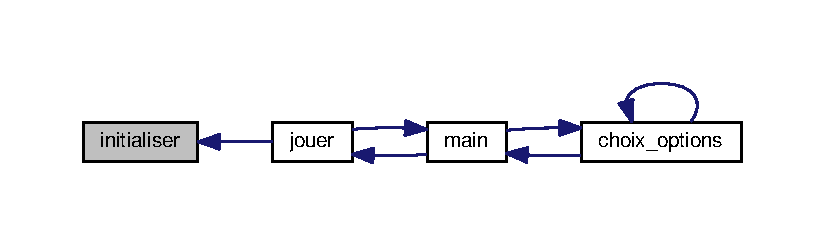
\includegraphics[width=350pt]{initialiser__background_8c_a627e8dbcc77f69a29241e6dccf38d77d_icgraph}
\end{center}
\end{figure}



\hypertarget{initialiser__ojbets_8c}{}\section{initialiser\+\_\+ojbets.\+c File Reference}
\label{initialiser__ojbets_8c}\index{initialiser\+\_\+ojbets.\+c@{initialiser\+\_\+ojbets.\+c}}
{\ttfamily \#include $<$stdlib.\+h$>$}\\*
{\ttfamily \#include $<$stdio.\+h$>$}\\*
{\ttfamily \#include $<$S\+D\+L/\+S\+D\+L.\+h$>$}\\*
{\ttfamily \#include \char`\"{}jouer.\+h\char`\"{}}\\*
Include dependency graph for initialiser\+\_\+ojbets.\+c\+:
\nopagebreak
\begin{figure}[H]
\begin{center}
\leavevmode
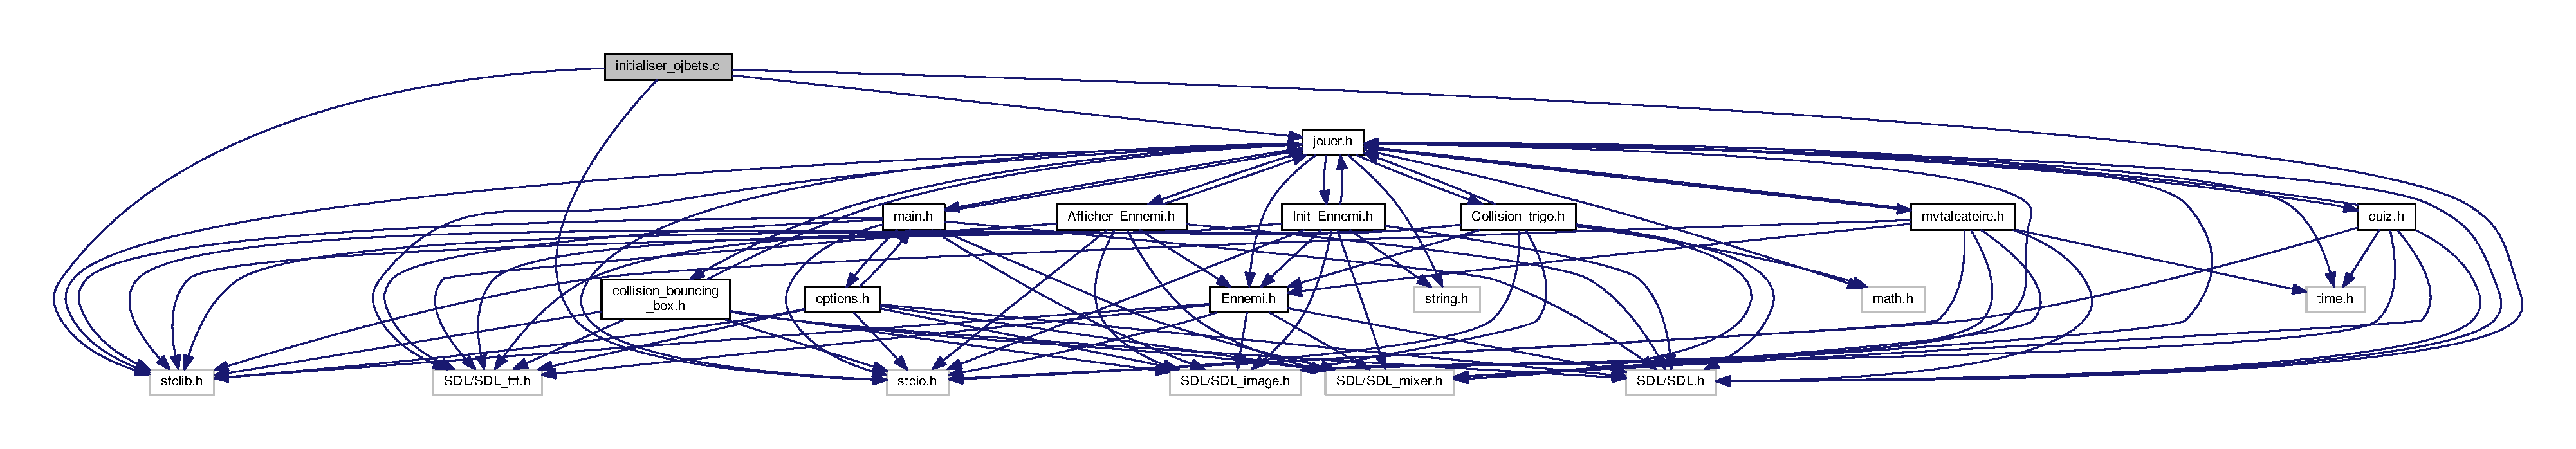
\includegraphics[width=350pt]{initialiser__ojbets_8c__incl}
\end{center}
\end{figure}
\subsection*{Functions}
\begin{DoxyCompactItemize}
\item 
void \hyperlink{initialiser__ojbets_8c_a86f775c18541dd59fc0bd67da6884963}{Initial\+\_\+objet} (\hyperlink{structEO}{EO} $\ast$ob, \hyperlink{structEO}{EO} $\ast$clef, \hyperlink{structEO}{EO} $\ast$porte, \hyperlink{structEO}{EO} $\ast$piste)
\end{DoxyCompactItemize}


\subsection{Function Documentation}
\index{initialiser\+\_\+ojbets.\+c@{initialiser\+\_\+ojbets.\+c}!Initial\+\_\+objet@{Initial\+\_\+objet}}
\index{Initial\+\_\+objet@{Initial\+\_\+objet}!initialiser\+\_\+ojbets.\+c@{initialiser\+\_\+ojbets.\+c}}
\subsubsection[{\texorpdfstring{Initial\+\_\+objet(\+E\+O $\ast$ob, E\+O $\ast$clef, E\+O $\ast$porte, E\+O $\ast$piste)}{Initial_objet(EO *ob, EO *clef, EO *porte, EO *piste)}}]{\setlength{\rightskip}{0pt plus 5cm}void Initial\+\_\+objet (
\begin{DoxyParamCaption}
\item[{{\bf EO} $\ast$}]{ob, }
\item[{{\bf EO} $\ast$}]{clef, }
\item[{{\bf EO} $\ast$}]{porte, }
\item[{{\bf EO} $\ast$}]{piste}
\end{DoxyParamCaption}
)}\hypertarget{initialiser__ojbets_8c_a86f775c18541dd59fc0bd67da6884963}{}\label{initialiser__ojbets_8c_a86f775c18541dd59fc0bd67da6884963}


Here is the caller graph for this function\+:
\nopagebreak
\begin{figure}[H]
\begin{center}
\leavevmode
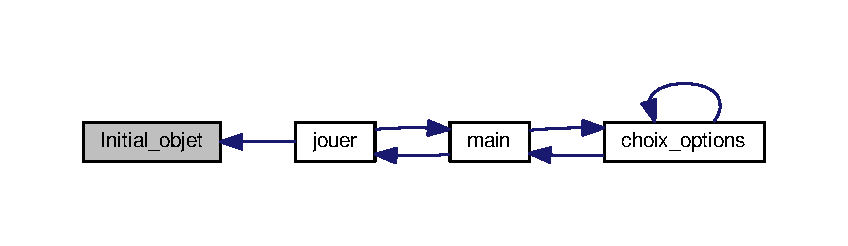
\includegraphics[width=350pt]{initialiser__ojbets_8c_a86f775c18541dd59fc0bd67da6884963_icgraph}
\end{center}
\end{figure}



\hypertarget{jouer_8c}{}\section{jouer.\+c File Reference}
\label{jouer_8c}\index{jouer.\+c@{jouer.\+c}}


Testing Program.  


{\ttfamily \#include $<$stdlib.\+h$>$}\\*
{\ttfamily \#include $<$stdio.\+h$>$}\\*
{\ttfamily \#include $<$S\+D\+L/\+S\+D\+L.\+h$>$}\\*
{\ttfamily \#include \char`\"{}jouer.\+h\char`\"{}}\\*
Include dependency graph for jouer.\+c\+:
\nopagebreak
\begin{figure}[H]
\begin{center}
\leavevmode
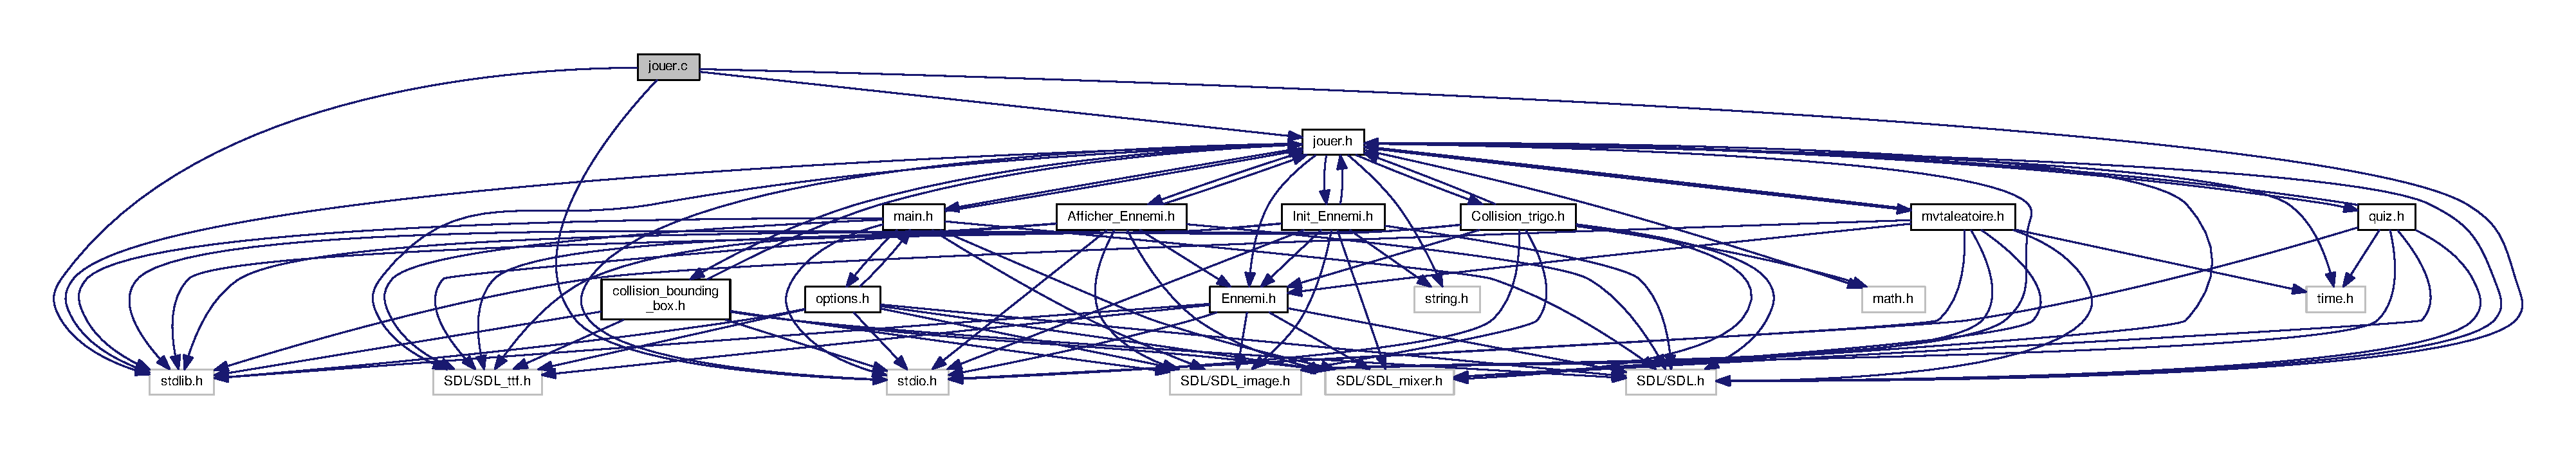
\includegraphics[width=350pt]{jouer_8c__incl}
\end{center}
\end{figure}
\subsection*{Functions}
\begin{DoxyCompactItemize}
\item 
void \hyperlink{jouer_8c_ad213c186f0cdc96ff9980238c752ac7c}{jouer} (S\+D\+L\+\_\+\+Surface $\ast$ecran)
\item 
void \hyperlink{jouer_8c_a9104e461369cd1360ebfae450d4a49e6}{Nettoyer\+\_\+stage} (S\+D\+L\+\_\+\+Surface $\ast$ecran)
\end{DoxyCompactItemize}


\subsection{Detailed Description}
Testing Program. 

\begin{DoxyAuthor}{Author}
C Team 
\end{DoxyAuthor}
\begin{DoxyVersion}{Version}
1.\+2 
\end{DoxyVersion}
\begin{DoxyDate}{Date}
Apr 04, 2019
\end{DoxyDate}
Testing program for game 

\subsection{Function Documentation}
\index{jouer.\+c@{jouer.\+c}!jouer@{jouer}}
\index{jouer@{jouer}!jouer.\+c@{jouer.\+c}}
\subsubsection[{\texorpdfstring{jouer(\+S\+D\+L\+\_\+\+Surface $\ast$ecran)}{jouer(SDL_Surface *ecran)}}]{\setlength{\rightskip}{0pt plus 5cm}void jouer (
\begin{DoxyParamCaption}
\item[{S\+D\+L\+\_\+\+Surface $\ast$}]{ecran}
\end{DoxyParamCaption}
)}\hypertarget{jouer_8c_ad213c186f0cdc96ff9980238c752ac7c}{}\label{jouer_8c_ad213c186f0cdc96ff9980238c752ac7c}


Here is the call graph for this function\+:
\nopagebreak
\begin{figure}[H]
\begin{center}
\leavevmode
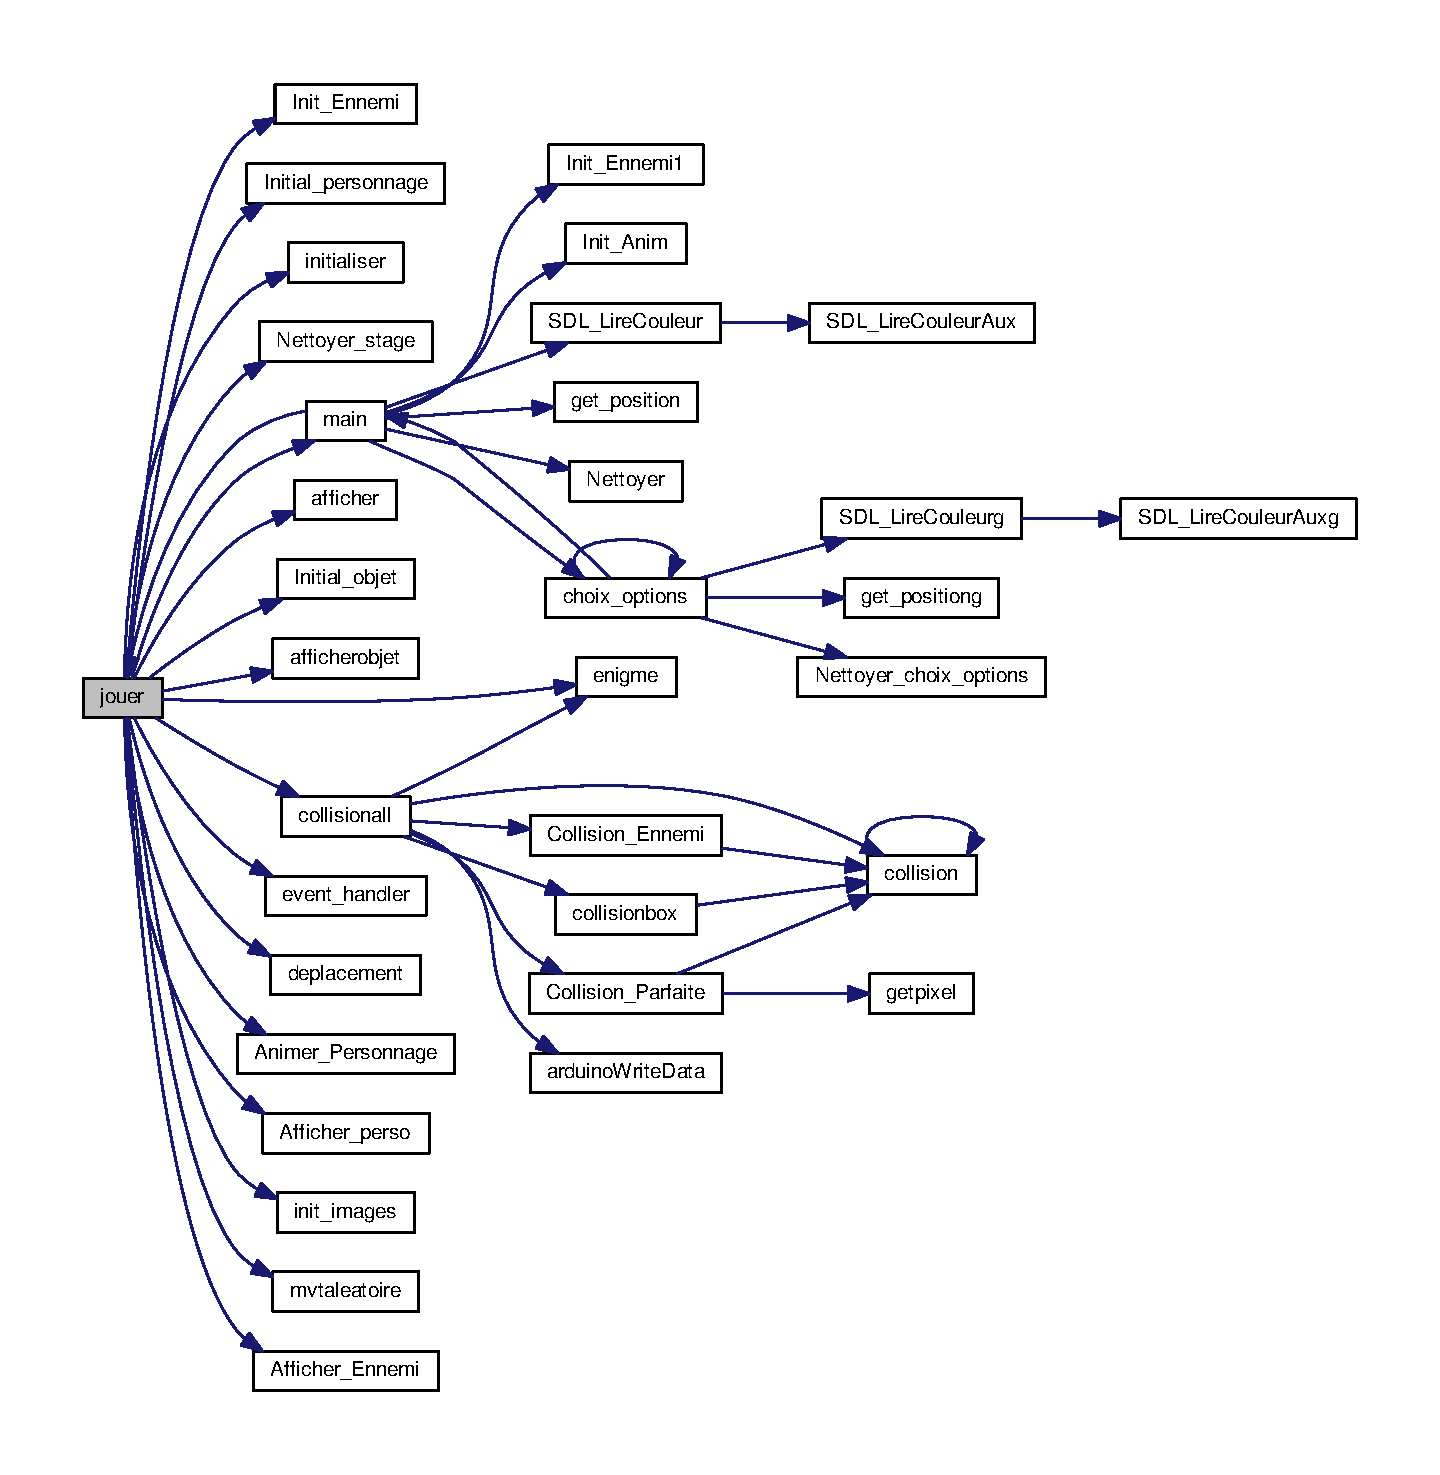
\includegraphics[width=350pt]{jouer_8c_ad213c186f0cdc96ff9980238c752ac7c_cgraph}
\end{center}
\end{figure}




Here is the caller graph for this function\+:
\nopagebreak
\begin{figure}[H]
\begin{center}
\leavevmode
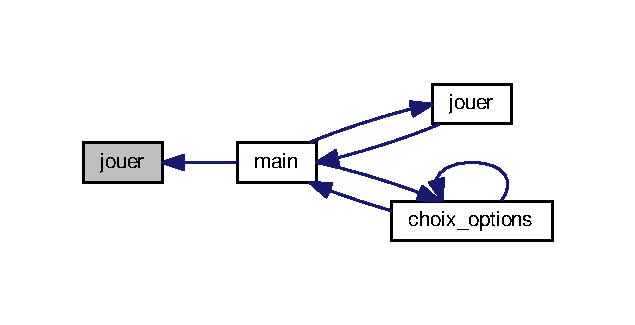
\includegraphics[width=305pt]{jouer_8c_ad213c186f0cdc96ff9980238c752ac7c_icgraph}
\end{center}
\end{figure}


\index{jouer.\+c@{jouer.\+c}!Nettoyer\+\_\+stage@{Nettoyer\+\_\+stage}}
\index{Nettoyer\+\_\+stage@{Nettoyer\+\_\+stage}!jouer.\+c@{jouer.\+c}}
\subsubsection[{\texorpdfstring{Nettoyer\+\_\+stage(\+S\+D\+L\+\_\+\+Surface $\ast$ecran)}{Nettoyer_stage(SDL_Surface *ecran)}}]{\setlength{\rightskip}{0pt plus 5cm}void Nettoyer\+\_\+stage (
\begin{DoxyParamCaption}
\item[{S\+D\+L\+\_\+\+Surface $\ast$}]{ecran}
\end{DoxyParamCaption}
)}\hypertarget{jouer_8c_a9104e461369cd1360ebfae450d4a49e6}{}\label{jouer_8c_a9104e461369cd1360ebfae450d4a49e6}


Here is the caller graph for this function\+:
\nopagebreak
\begin{figure}[H]
\begin{center}
\leavevmode
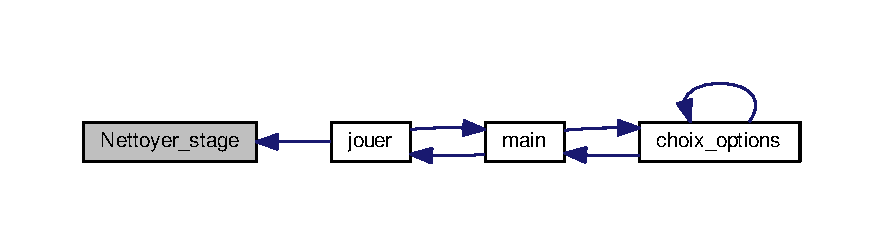
\includegraphics[width=350pt]{jouer_8c_a9104e461369cd1360ebfae450d4a49e6_icgraph}
\end{center}
\end{figure}



\hypertarget{jouer_8h}{}\section{jouer.\+h File Reference}
\label{jouer_8h}\index{jouer.\+h@{jouer.\+h}}
{\ttfamily \#include $<$stdlib.\+h$>$}\\*
{\ttfamily \#include $<$stdio.\+h$>$}\\*
{\ttfamily \#include $<$math.\+h$>$}\\*
{\ttfamily \#include $<$time.\+h$>$}\\*
{\ttfamily \#include $<$string.\+h$>$}\\*
{\ttfamily \#include $<$S\+D\+L/\+S\+D\+L.\+h$>$}\\*
{\ttfamily \#include $<$S\+D\+L/\+S\+D\+L\+\_\+image.\+h$>$}\\*
{\ttfamily \#include $<$S\+D\+L/\+S\+D\+L\+\_\+mixer.\+h$>$}\\*
{\ttfamily \#include $<$S\+D\+L/\+S\+D\+L\+\_\+ttf.\+h$>$}\\*
{\ttfamily \#include \char`\"{}collision\+\_\+bounding\+\_\+box.\+h\char`\"{}}\\*
{\ttfamily \#include \char`\"{}Init\+\_\+\+Ennemi.\+h\char`\"{}}\\*
{\ttfamily \#include \char`\"{}Afficher\+\_\+\+Ennemi.\+h\char`\"{}}\\*
{\ttfamily \#include \char`\"{}mvtaleatoire.\+h\char`\"{}}\\*
{\ttfamily \#include \char`\"{}Ennemi.\+h\char`\"{}}\\*
{\ttfamily \#include \char`\"{}main.\+h\char`\"{}}\\*
{\ttfamily \#include \char`\"{}Collision\+\_\+trigo.\+h\char`\"{}}\\*
{\ttfamily \#include \char`\"{}quiz.\+h\char`\"{}}\\*
Include dependency graph for jouer.\+h\+:
\nopagebreak
\begin{figure}[H]
\begin{center}
\leavevmode
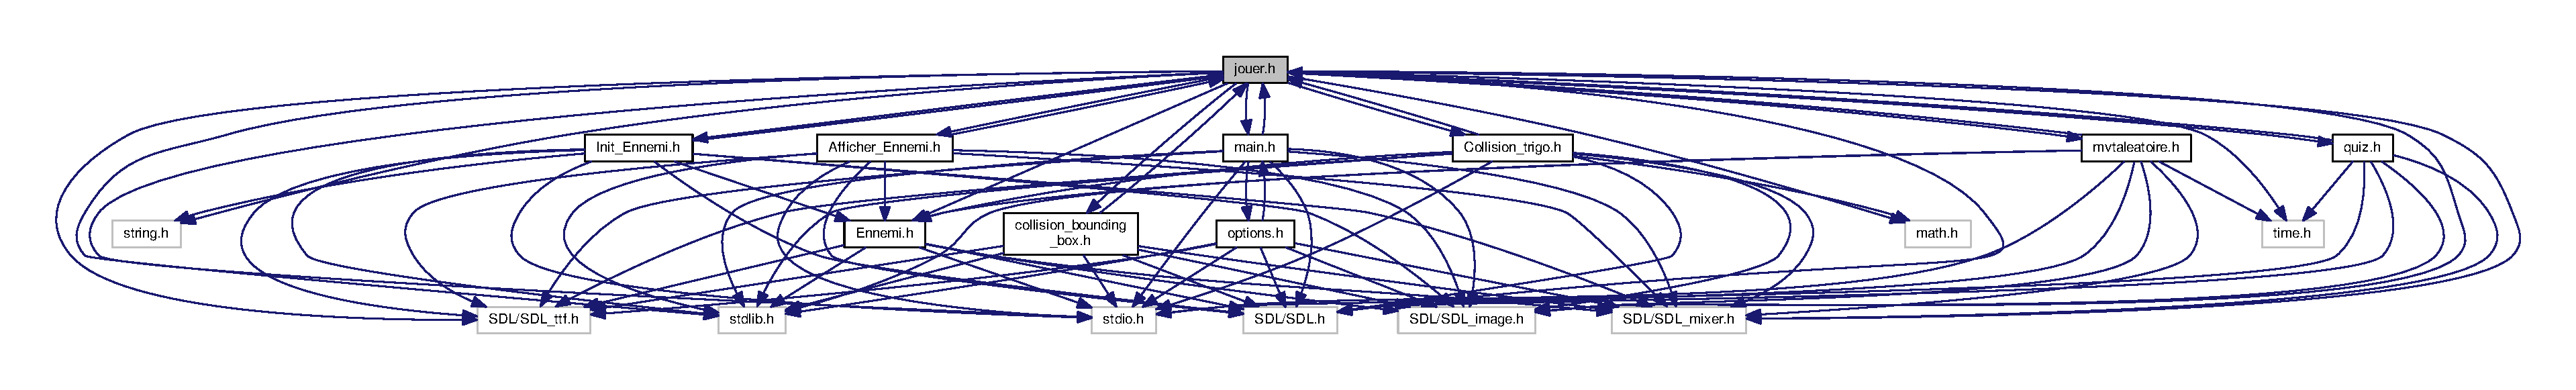
\includegraphics[width=350pt]{jouer_8h__incl}
\end{center}
\end{figure}
This graph shows which files directly or indirectly include this file\+:
\nopagebreak
\begin{figure}[H]
\begin{center}
\leavevmode
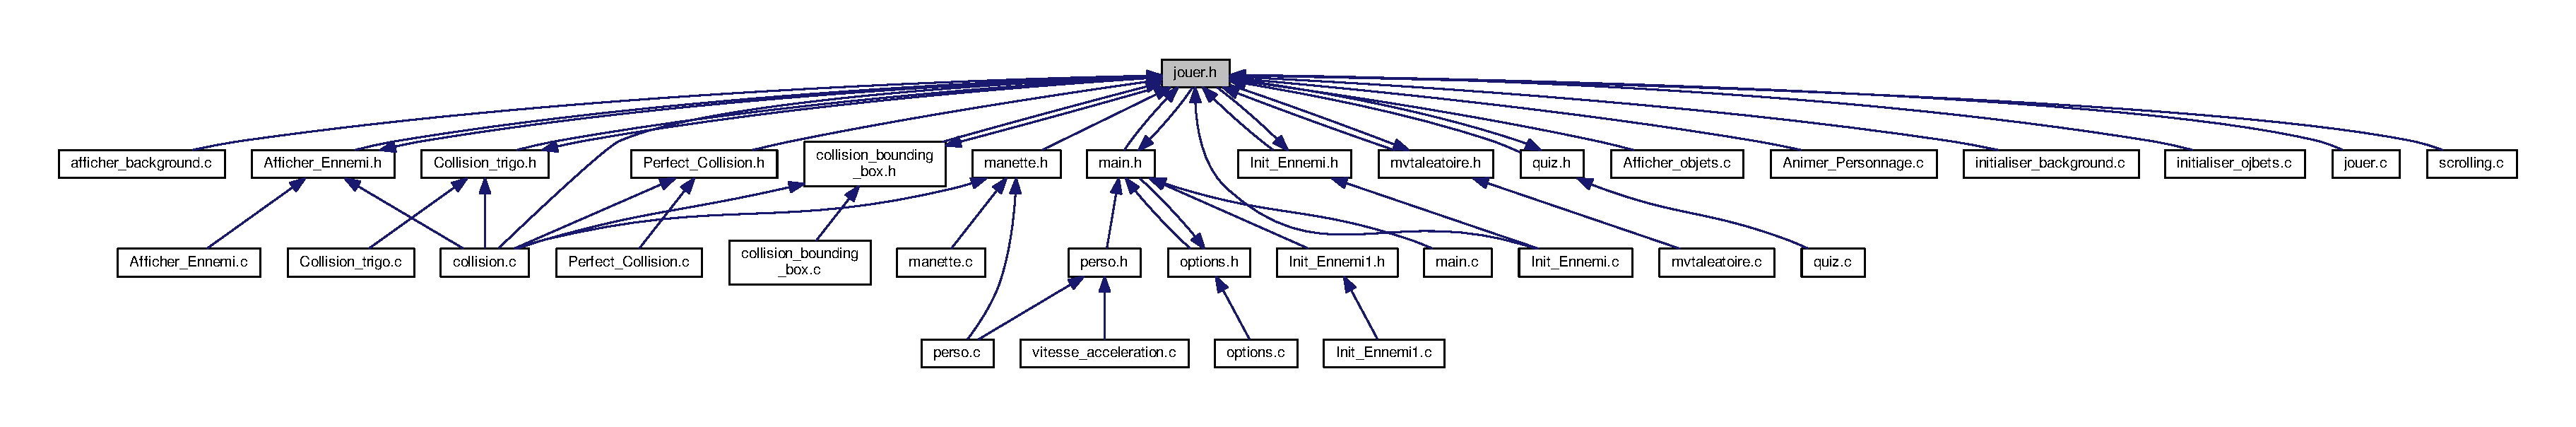
\includegraphics[width=350pt]{jouer_8h__dep__incl}
\end{center}
\end{figure}
\subsection*{Classes}
\begin{DoxyCompactItemize}
\item 
struct \hyperlink{structCoordinate}{Coordinate}
\item 
struct \hyperlink{structbackground}{background}
\item 
struct \hyperlink{structPlayer}{Player}
\item 
struct \hyperlink{structEO}{EO}
\end{DoxyCompactItemize}
\subsection*{Typedefs}
\begin{DoxyCompactItemize}
\item 
typedef struct \hyperlink{structPlayer}{Player} \hyperlink{jouer_8h_a480a040facb94f90060562cd65274385}{Player}
\item 
typedef struct \hyperlink{structEO}{EO} \hyperlink{jouer_8h_ae2c08096f52a2326f5d7dac728eba859}{EO}
\end{DoxyCompactItemize}
\subsection*{Enumerations}
\begin{DoxyCompactItemize}
\item 
enum \hyperlink{jouer_8h_a767b7a63d7677f92d697621b4166af1b}{Etat} \{ \hyperlink{jouer_8h_a767b7a63d7677f92d697621b4166af1ba831c130f9c83adc963152d232a9d61c7}{A\+T\+T\+A\+CK}, 
\hyperlink{jouer_8h_a767b7a63d7677f92d697621b4166af1bafd6a0e4343048b10646dd2976cc5ad18}{I\+D\+LE}, 
\hyperlink{jouer_8h_a767b7a63d7677f92d697621b4166af1bafdb9f1cb7b335ece267de4cd11688bfa}{W\+A\+LK}
 \}
\item 
enum \hyperlink{jouer_8h_a224b9163917ac32fc95a60d8c1eec3aa}{Direction} \{ \hyperlink{jouer_8h_a224b9163917ac32fc95a60d8c1eec3aaaba595d8bca8bc5e67c37c0a9d89becfa}{UP}, 
\hyperlink{jouer_8h_a224b9163917ac32fc95a60d8c1eec3aaa9b0b4a95b99523966e0e34ffdadac9da}{D\+O\+WN}, 
\hyperlink{jouer_8h_a224b9163917ac32fc95a60d8c1eec3aaaec8379af7490bb9eaaf579cf17876f38}{R\+I\+G\+HT}, 
\hyperlink{jouer_8h_a224b9163917ac32fc95a60d8c1eec3aaadb45120aafd37a973140edee24708065}{L\+E\+FT}
 \}
\end{DoxyCompactItemize}
\subsection*{Functions}
\begin{DoxyCompactItemize}
\item 
void \hyperlink{jouer_8h_a627e8dbcc77f69a29241e6dccf38d77d}{initialiser} (\hyperlink{structbackground}{background} $\ast$b)
\item 
void \hyperlink{jouer_8h_ad5e245ac884b3a5bc774dca864a5e0c0}{afficher} (S\+D\+L\+\_\+\+Surface $\ast$ecran, \hyperlink{structbackground}{background} $\ast$b)
\item 
\hyperlink{structPlayer}{Player} \hyperlink{jouer_8h_a7fcb81f452dcbccb499a3ce85062d589}{Initial\+\_\+personnage} ()
\item 
void \hyperlink{jouer_8h_a72fcd39f3658ec12884bd69a639359ee}{event\+\_\+handler} (S\+D\+L\+\_\+\+Event event, \hyperlink{jouer_8h_a224b9163917ac32fc95a60d8c1eec3aa}{Direction} $\ast$Sens, \hyperlink{jouer_8h_a767b7a63d7677f92d697621b4166af1b}{Etat} $\ast$State, int $\ast$keys\+Held)
\item 
void \hyperlink{jouer_8h_aff1748dab6c55558808b6a23b947f974}{deplacement} (\hyperlink{jouer_8h_a224b9163917ac32fc95a60d8c1eec3aa}{Direction} Sens, \hyperlink{jouer_8h_a767b7a63d7677f92d697621b4166af1b}{Etat} State, \hyperlink{structPlayer}{Player} $\ast$hero, int $\ast$keys\+Held)
\item 
void \hyperlink{jouer_8h_aadd479ddab8191523cfee947e8a718b1}{Afficher\+\_\+perso} (\hyperlink{structPlayer}{Player} hero, int vie, S\+D\+L\+\_\+\+Surface $\ast$ecran)
\item 
void \hyperlink{jouer_8h_a3dc3993bdcecc71ad5576c072f25e29d}{Animer\+\_\+\+Personnage} (int $\ast$frametime, int nmb\+\_\+frame, int $\ast$frame, \hyperlink{structPlayer}{Player} $\ast$hero, \hyperlink{jouer_8h_a224b9163917ac32fc95a60d8c1eec3aa}{Direction} $\ast$Sens, \hyperlink{jouer_8h_a767b7a63d7677f92d697621b4166af1b}{Etat} $\ast$State)
\item 
void \hyperlink{jouer_8h_a86f775c18541dd59fc0bd67da6884963}{Initial\+\_\+objet} (\hyperlink{structEO}{EO} $\ast$ob, \hyperlink{structEO}{EO} $\ast$clef, \hyperlink{structEO}{EO} $\ast$porte, \hyperlink{structEO}{EO} $\ast$piste)
\item 
void \hyperlink{jouer_8h_a42cab3047c025df170f86a167a498c40}{afficherobjet} (\hyperlink{structEO}{EO} $\ast$ob, \hyperlink{structEO}{EO} $\ast$clef, \hyperlink{structEO}{EO} $\ast$porte, \hyperlink{structEO}{EO} $\ast$piste, S\+D\+L\+\_\+\+Surface $\ast$ecran, \hyperlink{structbackground}{background} $\ast$b)
\item 
void \hyperlink{jouer_8h_a81c2e8441b67355bf2c68a5c0fa4d2d6}{scrolling} (\hyperlink{structbackground}{background} $\ast$b, S\+D\+L\+\_\+\+Surface $\ast$ecran, \hyperlink{jouer_8h_a224b9163917ac32fc95a60d8c1eec3aa}{Direction} Sens, \hyperlink{jouer_8h_a767b7a63d7677f92d697621b4166af1b}{Etat} State)
\item 
int \hyperlink{jouer_8h_aaf6f1dec5bb7d4e93d8d580a8e550442}{collision} (S\+D\+L\+\_\+\+Surface $\ast$p, S\+D\+L\+\_\+\+Surface $\ast$e, S\+D\+L\+\_\+\+Rect perso, S\+D\+L\+\_\+\+Rect enemy)
\item 
int \hyperlink{jouer_8h_aada0004db077b368ab0b29a7f0e74d72}{collisionbox} (S\+D\+L\+\_\+\+Surface $\ast$p, S\+D\+L\+\_\+\+Surface $\ast$o, S\+D\+L\+\_\+\+Rect perso, S\+D\+L\+\_\+\+Rect objet)
\item 
int \hyperlink{jouer_8h_a1201e4f88c0ee7608ca131ce01681997}{collisionall} (\hyperlink{structEO}{EO} $\ast$ob, \hyperlink{structEO}{EO} clef, \hyperlink{structEO}{EO} porte, \hyperlink{structEO}{EO} piste, \hyperlink{structPlayer}{Player} $\ast$hero, int $\ast$vie, int $\ast$score, \hyperlink{jouer_8h_a224b9163917ac32fc95a60d8c1eec3aa}{Direction} Sens, \hyperlink{jouer_8h_a767b7a63d7677f92d697621b4166af1b}{Etat} State, \hyperlink{structEnnemi}{Ennemi} Mob\mbox{[}$\,$\mbox{]}, \hyperlink{structCoordinate}{Coordinate} C, S\+D\+L\+\_\+\+Surface $\ast$Background)
\item 
int \hyperlink{jouer_8h_aa7a006f89e162da81cf20be078bf3653}{Collision\+\_\+\+Ennemi} (S\+D\+L\+\_\+\+Rect Pos\+\_\+perso, \hyperlink{structEnnemi}{Ennemi} Mob)
\item 
\hyperlink{structEnnemi}{Ennemi} \hyperlink{jouer_8h_acc0a5eae1c2488e30bf55a4b064cc833}{Init\+\_\+\+Ennemi} (char Mob\+\_\+\+Name\mbox{[}$\,$\mbox{]}, int X, int Y)
\item 
void \hyperlink{jouer_8h_a5bd3b2cfb590a56ce994b524cd23e1aa}{Afficher\+\_\+\+Ennemi} (\hyperlink{structEnnemi}{Ennemi} Mob, S\+D\+L\+\_\+\+Surface $\ast$ecran)
\item 
void \hyperlink{jouer_8h_afc8b6113658127f5da2f173a2f07d697}{mvtaleatoire} (\hyperlink{structEnnemi}{Ennemi} $\ast$mob, int max, int min)
\item 
void \hyperlink{jouer_8h_a17f70e17a66034ab2cfe4ecd23d0a96a}{enigme} (int d, S\+D\+L\+\_\+\+Surface $\ast$ecran)
\item 
void \hyperlink{jouer_8h_a313b3d1a9789026d9311ce31218dfddc}{reponse} (S\+D\+L\+\_\+\+Surface $\ast$ecran, int d)
\item 
void \hyperlink{jouer_8h_a2774260562b0dca66057190a74a45edb}{solution} (S\+D\+L\+\_\+\+Surface $\ast$ecran, int d)
\item 
void \hyperlink{jouer_8h_aec72a4538c45c4b123f92b3aa554980a}{quiz} (S\+D\+L\+\_\+\+Surface $\ast$ecran, int d)
\item 
void \hyperlink{jouer_8h_a7dd2f18aee0b8b5e643a0817ad685d34}{good} (S\+D\+L\+\_\+\+Surface $\ast$ecran)
\item 
void \hyperlink{jouer_8h_ad213c186f0cdc96ff9980238c752ac7c}{jouer} (S\+D\+L\+\_\+\+Surface $\ast$ecran)
\item 
void \hyperlink{jouer_8h_a9104e461369cd1360ebfae450d4a49e6}{Nettoyer\+\_\+stage} (S\+D\+L\+\_\+\+Surface $\ast$ecran)
\item 
int \hyperlink{jouer_8h_a34cbc014d36b81852811368db4a70a98}{arduino\+Write\+Data} (int w)
\item 
int \hyperlink{jouer_8h_af26975b0e6c2018b62f8f188392ffba8}{arduino\+Read\+Data} (int $\ast$x)
\end{DoxyCompactItemize}


\subsection{Typedef Documentation}
\index{jouer.\+h@{jouer.\+h}!EO@{EO}}
\index{EO@{EO}!jouer.\+h@{jouer.\+h}}
\subsubsection[{\texorpdfstring{EO}{EO}}]{\setlength{\rightskip}{0pt plus 5cm}typedef struct {\bf EO} {\bf EO}}\hypertarget{jouer_8h_ae2c08096f52a2326f5d7dac728eba859}{}\label{jouer_8h_ae2c08096f52a2326f5d7dac728eba859}
\index{jouer.\+h@{jouer.\+h}!Player@{Player}}
\index{Player@{Player}!jouer.\+h@{jouer.\+h}}
\subsubsection[{\texorpdfstring{Player}{Player}}]{\setlength{\rightskip}{0pt plus 5cm}typedef struct {\bf Player} {\bf Player}}\hypertarget{jouer_8h_a480a040facb94f90060562cd65274385}{}\label{jouer_8h_a480a040facb94f90060562cd65274385}


\subsection{Enumeration Type Documentation}
\index{jouer.\+h@{jouer.\+h}!Direction@{Direction}}
\index{Direction@{Direction}!jouer.\+h@{jouer.\+h}}
\subsubsection[{\texorpdfstring{Direction}{Direction}}]{\setlength{\rightskip}{0pt plus 5cm}enum {\bf Direction}}\hypertarget{jouer_8h_a224b9163917ac32fc95a60d8c1eec3aa}{}\label{jouer_8h_a224b9163917ac32fc95a60d8c1eec3aa}
\begin{Desc}
\item[Enumerator]\par
\begin{description}
\index{UP@{UP}!jouer.\+h@{jouer.\+h}}\index{jouer.\+h@{jouer.\+h}!UP@{UP}}\item[{\em 
UP\hypertarget{jouer_8h_a224b9163917ac32fc95a60d8c1eec3aaaba595d8bca8bc5e67c37c0a9d89becfa}{}\label{jouer_8h_a224b9163917ac32fc95a60d8c1eec3aaaba595d8bca8bc5e67c37c0a9d89becfa}
}]\index{D\+O\+WN@{D\+O\+WN}!jouer.\+h@{jouer.\+h}}\index{jouer.\+h@{jouer.\+h}!D\+O\+WN@{D\+O\+WN}}\item[{\em 
D\+O\+WN\hypertarget{jouer_8h_a224b9163917ac32fc95a60d8c1eec3aaa9b0b4a95b99523966e0e34ffdadac9da}{}\label{jouer_8h_a224b9163917ac32fc95a60d8c1eec3aaa9b0b4a95b99523966e0e34ffdadac9da}
}]\index{R\+I\+G\+HT@{R\+I\+G\+HT}!jouer.\+h@{jouer.\+h}}\index{jouer.\+h@{jouer.\+h}!R\+I\+G\+HT@{R\+I\+G\+HT}}\item[{\em 
R\+I\+G\+HT\hypertarget{jouer_8h_a224b9163917ac32fc95a60d8c1eec3aaaec8379af7490bb9eaaf579cf17876f38}{}\label{jouer_8h_a224b9163917ac32fc95a60d8c1eec3aaaec8379af7490bb9eaaf579cf17876f38}
}]\index{L\+E\+FT@{L\+E\+FT}!jouer.\+h@{jouer.\+h}}\index{jouer.\+h@{jouer.\+h}!L\+E\+FT@{L\+E\+FT}}\item[{\em 
L\+E\+FT\hypertarget{jouer_8h_a224b9163917ac32fc95a60d8c1eec3aaadb45120aafd37a973140edee24708065}{}\label{jouer_8h_a224b9163917ac32fc95a60d8c1eec3aaadb45120aafd37a973140edee24708065}
}]\end{description}
\end{Desc}
\index{jouer.\+h@{jouer.\+h}!Etat@{Etat}}
\index{Etat@{Etat}!jouer.\+h@{jouer.\+h}}
\subsubsection[{\texorpdfstring{Etat}{Etat}}]{\setlength{\rightskip}{0pt plus 5cm}enum {\bf Etat}}\hypertarget{jouer_8h_a767b7a63d7677f92d697621b4166af1b}{}\label{jouer_8h_a767b7a63d7677f92d697621b4166af1b}
\begin{Desc}
\item[Enumerator]\par
\begin{description}
\index{A\+T\+T\+A\+CK@{A\+T\+T\+A\+CK}!jouer.\+h@{jouer.\+h}}\index{jouer.\+h@{jouer.\+h}!A\+T\+T\+A\+CK@{A\+T\+T\+A\+CK}}\item[{\em 
A\+T\+T\+A\+CK\hypertarget{jouer_8h_a767b7a63d7677f92d697621b4166af1ba831c130f9c83adc963152d232a9d61c7}{}\label{jouer_8h_a767b7a63d7677f92d697621b4166af1ba831c130f9c83adc963152d232a9d61c7}
}]\index{I\+D\+LE@{I\+D\+LE}!jouer.\+h@{jouer.\+h}}\index{jouer.\+h@{jouer.\+h}!I\+D\+LE@{I\+D\+LE}}\item[{\em 
I\+D\+LE\hypertarget{jouer_8h_a767b7a63d7677f92d697621b4166af1bafd6a0e4343048b10646dd2976cc5ad18}{}\label{jouer_8h_a767b7a63d7677f92d697621b4166af1bafd6a0e4343048b10646dd2976cc5ad18}
}]\index{W\+A\+LK@{W\+A\+LK}!jouer.\+h@{jouer.\+h}}\index{jouer.\+h@{jouer.\+h}!W\+A\+LK@{W\+A\+LK}}\item[{\em 
W\+A\+LK\hypertarget{jouer_8h_a767b7a63d7677f92d697621b4166af1bafdb9f1cb7b335ece267de4cd11688bfa}{}\label{jouer_8h_a767b7a63d7677f92d697621b4166af1bafdb9f1cb7b335ece267de4cd11688bfa}
}]\end{description}
\end{Desc}


\subsection{Function Documentation}
\index{jouer.\+h@{jouer.\+h}!afficher@{afficher}}
\index{afficher@{afficher}!jouer.\+h@{jouer.\+h}}
\subsubsection[{\texorpdfstring{afficher(\+S\+D\+L\+\_\+\+Surface $\ast$ecran, background $\ast$b)}{afficher(SDL_Surface *ecran, background *b)}}]{\setlength{\rightskip}{0pt plus 5cm}void afficher (
\begin{DoxyParamCaption}
\item[{S\+D\+L\+\_\+\+Surface $\ast$}]{ecran, }
\item[{{\bf background} $\ast$}]{b}
\end{DoxyParamCaption}
)}\hypertarget{jouer_8h_ad5e245ac884b3a5bc774dca864a5e0c0}{}\label{jouer_8h_ad5e245ac884b3a5bc774dca864a5e0c0}


Here is the caller graph for this function\+:
\nopagebreak
\begin{figure}[H]
\begin{center}
\leavevmode
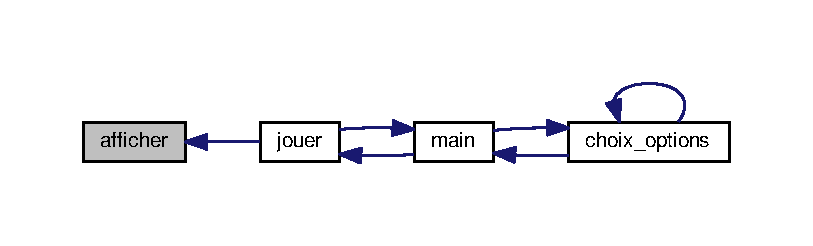
\includegraphics[width=350pt]{jouer_8h_ad5e245ac884b3a5bc774dca864a5e0c0_icgraph}
\end{center}
\end{figure}


\index{jouer.\+h@{jouer.\+h}!Afficher\+\_\+\+Ennemi@{Afficher\+\_\+\+Ennemi}}
\index{Afficher\+\_\+\+Ennemi@{Afficher\+\_\+\+Ennemi}!jouer.\+h@{jouer.\+h}}
\subsubsection[{\texorpdfstring{Afficher\+\_\+\+Ennemi(\+Ennemi Mob, S\+D\+L\+\_\+\+Surface $\ast$ecran)}{Afficher_Ennemi(Ennemi Mob, SDL_Surface *ecran)}}]{\setlength{\rightskip}{0pt plus 5cm}void Afficher\+\_\+\+Ennemi (
\begin{DoxyParamCaption}
\item[{{\bf Ennemi}}]{Mob, }
\item[{S\+D\+L\+\_\+\+Surface $\ast$}]{ecran}
\end{DoxyParamCaption}
)}\hypertarget{jouer_8h_a5bd3b2cfb590a56ce994b524cd23e1aa}{}\label{jouer_8h_a5bd3b2cfb590a56ce994b524cd23e1aa}


Here is the caller graph for this function\+:
\nopagebreak
\begin{figure}[H]
\begin{center}
\leavevmode
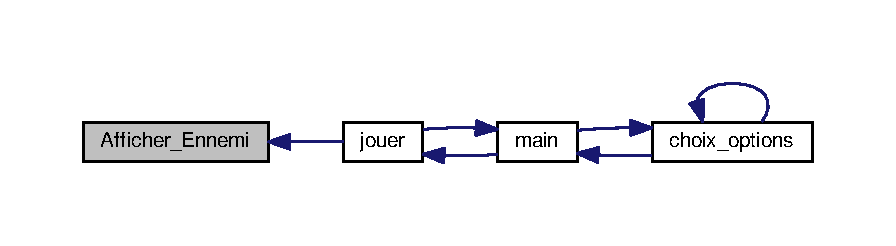
\includegraphics[width=350pt]{jouer_8h_a5bd3b2cfb590a56ce994b524cd23e1aa_icgraph}
\end{center}
\end{figure}


\index{jouer.\+h@{jouer.\+h}!Afficher\+\_\+perso@{Afficher\+\_\+perso}}
\index{Afficher\+\_\+perso@{Afficher\+\_\+perso}!jouer.\+h@{jouer.\+h}}
\subsubsection[{\texorpdfstring{Afficher\+\_\+perso(\+Player hero, int vie, S\+D\+L\+\_\+\+Surface $\ast$ecran)}{Afficher_perso(Player hero, int vie, SDL_Surface *ecran)}}]{\setlength{\rightskip}{0pt plus 5cm}void Afficher\+\_\+perso (
\begin{DoxyParamCaption}
\item[{{\bf Player}}]{hero, }
\item[{int}]{vie, }
\item[{S\+D\+L\+\_\+\+Surface $\ast$}]{ecran}
\end{DoxyParamCaption}
)}\hypertarget{jouer_8h_aadd479ddab8191523cfee947e8a718b1}{}\label{jouer_8h_aadd479ddab8191523cfee947e8a718b1}


Here is the caller graph for this function\+:
\nopagebreak
\begin{figure}[H]
\begin{center}
\leavevmode
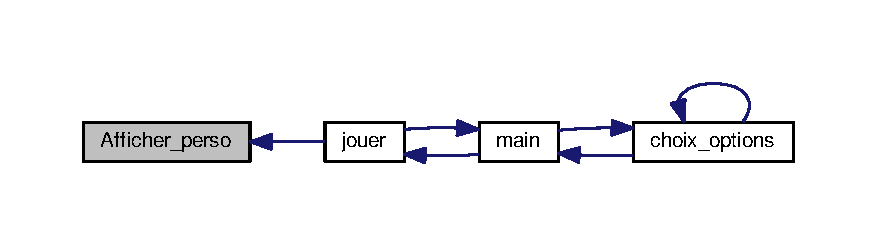
\includegraphics[width=350pt]{jouer_8h_aadd479ddab8191523cfee947e8a718b1_icgraph}
\end{center}
\end{figure}


\index{jouer.\+h@{jouer.\+h}!afficherobjet@{afficherobjet}}
\index{afficherobjet@{afficherobjet}!jouer.\+h@{jouer.\+h}}
\subsubsection[{\texorpdfstring{afficherobjet(\+E\+O $\ast$ob, E\+O $\ast$clef, E\+O $\ast$porte, E\+O $\ast$piste, S\+D\+L\+\_\+\+Surface $\ast$ecran, background $\ast$b)}{afficherobjet(EO *ob, EO *clef, EO *porte, EO *piste, SDL_Surface *ecran, background *b)}}]{\setlength{\rightskip}{0pt plus 5cm}void afficherobjet (
\begin{DoxyParamCaption}
\item[{{\bf EO} $\ast$}]{ob, }
\item[{{\bf EO} $\ast$}]{clef, }
\item[{{\bf EO} $\ast$}]{porte, }
\item[{{\bf EO} $\ast$}]{piste, }
\item[{S\+D\+L\+\_\+\+Surface $\ast$}]{ecran, }
\item[{{\bf background} $\ast$}]{b}
\end{DoxyParamCaption}
)}\hypertarget{jouer_8h_a42cab3047c025df170f86a167a498c40}{}\label{jouer_8h_a42cab3047c025df170f86a167a498c40}


Here is the caller graph for this function\+:
\nopagebreak
\begin{figure}[H]
\begin{center}
\leavevmode
\includegraphics[width=350pt]{jouer_8h_a42cab3047c025df170f86a167a498c40_icgraph}
\end{center}
\end{figure}


\index{jouer.\+h@{jouer.\+h}!Animer\+\_\+\+Personnage@{Animer\+\_\+\+Personnage}}
\index{Animer\+\_\+\+Personnage@{Animer\+\_\+\+Personnage}!jouer.\+h@{jouer.\+h}}
\subsubsection[{\texorpdfstring{Animer\+\_\+\+Personnage(int $\ast$frametime, int nmb\+\_\+frame, int $\ast$frame, Player $\ast$hero, Direction $\ast$\+Sens, Etat $\ast$\+State)}{Animer_Personnage(int *frametime, int nmb_frame, int *frame, Player *hero, Direction *Sens, Etat *State)}}]{\setlength{\rightskip}{0pt plus 5cm}void Animer\+\_\+\+Personnage (
\begin{DoxyParamCaption}
\item[{int $\ast$}]{frametime, }
\item[{int}]{nmb\+\_\+frame, }
\item[{int $\ast$}]{frame, }
\item[{{\bf Player} $\ast$}]{hero, }
\item[{{\bf Direction} $\ast$}]{Sens, }
\item[{{\bf Etat} $\ast$}]{State}
\end{DoxyParamCaption}
)}\hypertarget{jouer_8h_a3dc3993bdcecc71ad5576c072f25e29d}{}\label{jouer_8h_a3dc3993bdcecc71ad5576c072f25e29d}


Here is the caller graph for this function\+:
\nopagebreak
\begin{figure}[H]
\begin{center}
\leavevmode
\includegraphics[width=350pt]{jouer_8h_a3dc3993bdcecc71ad5576c072f25e29d_icgraph}
\end{center}
\end{figure}


\index{jouer.\+h@{jouer.\+h}!arduino\+Read\+Data@{arduino\+Read\+Data}}
\index{arduino\+Read\+Data@{arduino\+Read\+Data}!jouer.\+h@{jouer.\+h}}
\subsubsection[{\texorpdfstring{arduino\+Read\+Data(int $\ast$x)}{arduinoReadData(int *x)}}]{\setlength{\rightskip}{0pt plus 5cm}int arduino\+Read\+Data (
\begin{DoxyParamCaption}
\item[{int $\ast$}]{x}
\end{DoxyParamCaption}
)}\hypertarget{jouer_8h_af26975b0e6c2018b62f8f188392ffba8}{}\label{jouer_8h_af26975b0e6c2018b62f8f188392ffba8}
\index{jouer.\+h@{jouer.\+h}!arduino\+Write\+Data@{arduino\+Write\+Data}}
\index{arduino\+Write\+Data@{arduino\+Write\+Data}!jouer.\+h@{jouer.\+h}}
\subsubsection[{\texorpdfstring{arduino\+Write\+Data(int w)}{arduinoWriteData(int w)}}]{\setlength{\rightskip}{0pt plus 5cm}int arduino\+Write\+Data (
\begin{DoxyParamCaption}
\item[{int}]{w}
\end{DoxyParamCaption}
)}\hypertarget{jouer_8h_a34cbc014d36b81852811368db4a70a98}{}\label{jouer_8h_a34cbc014d36b81852811368db4a70a98}


Here is the caller graph for this function\+:
\nopagebreak
\begin{figure}[H]
\begin{center}
\leavevmode
\includegraphics[width=350pt]{jouer_8h_a34cbc014d36b81852811368db4a70a98_icgraph}
\end{center}
\end{figure}


\index{jouer.\+h@{jouer.\+h}!collision@{collision}}
\index{collision@{collision}!jouer.\+h@{jouer.\+h}}
\subsubsection[{\texorpdfstring{collision(\+S\+D\+L\+\_\+\+Surface $\ast$p, S\+D\+L\+\_\+\+Surface $\ast$e, S\+D\+L\+\_\+\+Rect perso, S\+D\+L\+\_\+\+Rect enemy)}{collision(SDL_Surface *p, SDL_Surface *e, SDL_Rect perso, SDL_Rect enemy)}}]{\setlength{\rightskip}{0pt plus 5cm}int collision (
\begin{DoxyParamCaption}
\item[{S\+D\+L\+\_\+\+Surface $\ast$}]{p, }
\item[{S\+D\+L\+\_\+\+Surface $\ast$}]{e, }
\item[{S\+D\+L\+\_\+\+Rect}]{perso, }
\item[{S\+D\+L\+\_\+\+Rect}]{enemy}
\end{DoxyParamCaption}
)}\hypertarget{jouer_8h_aaf6f1dec5bb7d4e93d8d580a8e550442}{}\label{jouer_8h_aaf6f1dec5bb7d4e93d8d580a8e550442}


Here is the call graph for this function\+:
\nopagebreak
\begin{figure}[H]
\begin{center}
\leavevmode
\includegraphics[width=220pt]{jouer_8h_aaf6f1dec5bb7d4e93d8d580a8e550442_cgraph}
\end{center}
\end{figure}




Here is the caller graph for this function\+:
\nopagebreak
\begin{figure}[H]
\begin{center}
\leavevmode
\includegraphics[width=350pt]{jouer_8h_aaf6f1dec5bb7d4e93d8d580a8e550442_icgraph}
\end{center}
\end{figure}


\index{jouer.\+h@{jouer.\+h}!Collision\+\_\+\+Ennemi@{Collision\+\_\+\+Ennemi}}
\index{Collision\+\_\+\+Ennemi@{Collision\+\_\+\+Ennemi}!jouer.\+h@{jouer.\+h}}
\subsubsection[{\texorpdfstring{Collision\+\_\+\+Ennemi(\+S\+D\+L\+\_\+\+Rect Pos\+\_\+perso, Ennemi Mob)}{Collision_Ennemi(SDL_Rect Pos_perso, Ennemi Mob)}}]{\setlength{\rightskip}{0pt plus 5cm}int Collision\+\_\+\+Ennemi (
\begin{DoxyParamCaption}
\item[{S\+D\+L\+\_\+\+Rect}]{Pos\+\_\+perso, }
\item[{{\bf Ennemi}}]{Mob}
\end{DoxyParamCaption}
)}\hypertarget{jouer_8h_aa7a006f89e162da81cf20be078bf3653}{}\label{jouer_8h_aa7a006f89e162da81cf20be078bf3653}


Here is the call graph for this function\+:
\nopagebreak
\begin{figure}[H]
\begin{center}
\leavevmode
\includegraphics[width=260pt]{jouer_8h_aa7a006f89e162da81cf20be078bf3653_cgraph}
\end{center}
\end{figure}




Here is the caller graph for this function\+:
\nopagebreak
\begin{figure}[H]
\begin{center}
\leavevmode
\includegraphics[width=350pt]{jouer_8h_aa7a006f89e162da81cf20be078bf3653_icgraph}
\end{center}
\end{figure}


\index{jouer.\+h@{jouer.\+h}!collisionall@{collisionall}}
\index{collisionall@{collisionall}!jouer.\+h@{jouer.\+h}}
\subsubsection[{\texorpdfstring{collisionall(\+E\+O $\ast$ob, E\+O clef, E\+O porte, E\+O piste, Player $\ast$hero, int $\ast$vie, int $\ast$score, Direction Sens, Etat State, Ennemi Mob[], Coordinate C, S\+D\+L\+\_\+\+Surface $\ast$\+Background)}{collisionall(EO *ob, EO clef, EO porte, EO piste, Player *hero, int *vie, int *score, Direction Sens, Etat State, Ennemi Mob[], Coordinate C, SDL_Surface *Background)}}]{\setlength{\rightskip}{0pt plus 5cm}int collisionall (
\begin{DoxyParamCaption}
\item[{{\bf EO} $\ast$}]{ob, }
\item[{{\bf EO}}]{clef, }
\item[{{\bf EO}}]{porte, }
\item[{{\bf EO}}]{piste, }
\item[{{\bf Player} $\ast$}]{hero, }
\item[{int $\ast$}]{vie, }
\item[{int $\ast$}]{score, }
\item[{{\bf Direction}}]{Sens, }
\item[{{\bf Etat}}]{State, }
\item[{{\bf Ennemi}}]{Mob\mbox{[}$\,$\mbox{]}, }
\item[{{\bf Coordinate}}]{C, }
\item[{S\+D\+L\+\_\+\+Surface $\ast$}]{Background}
\end{DoxyParamCaption}
)}\hypertarget{jouer_8h_a1201e4f88c0ee7608ca131ce01681997}{}\label{jouer_8h_a1201e4f88c0ee7608ca131ce01681997}


Here is the call graph for this function\+:
\nopagebreak
\begin{figure}[H]
\begin{center}
\leavevmode
\includegraphics[width=350pt]{jouer_8h_a1201e4f88c0ee7608ca131ce01681997_cgraph}
\end{center}
\end{figure}




Here is the caller graph for this function\+:
\nopagebreak
\begin{figure}[H]
\begin{center}
\leavevmode
\includegraphics[width=350pt]{jouer_8h_a1201e4f88c0ee7608ca131ce01681997_icgraph}
\end{center}
\end{figure}


\index{jouer.\+h@{jouer.\+h}!collisionbox@{collisionbox}}
\index{collisionbox@{collisionbox}!jouer.\+h@{jouer.\+h}}
\subsubsection[{\texorpdfstring{collisionbox(\+S\+D\+L\+\_\+\+Surface $\ast$p, S\+D\+L\+\_\+\+Surface $\ast$o, S\+D\+L\+\_\+\+Rect perso, S\+D\+L\+\_\+\+Rect objet)}{collisionbox(SDL_Surface *p, SDL_Surface *o, SDL_Rect perso, SDL_Rect objet)}}]{\setlength{\rightskip}{0pt plus 5cm}int collisionbox (
\begin{DoxyParamCaption}
\item[{S\+D\+L\+\_\+\+Surface $\ast$}]{p, }
\item[{S\+D\+L\+\_\+\+Surface $\ast$}]{o, }
\item[{S\+D\+L\+\_\+\+Rect}]{perso, }
\item[{S\+D\+L\+\_\+\+Rect}]{objet}
\end{DoxyParamCaption}
)}\hypertarget{jouer_8h_aada0004db077b368ab0b29a7f0e74d72}{}\label{jouer_8h_aada0004db077b368ab0b29a7f0e74d72}


Here is the call graph for this function\+:
\nopagebreak
\begin{figure}[H]
\begin{center}
\leavevmode
\includegraphics[width=236pt]{jouer_8h_aada0004db077b368ab0b29a7f0e74d72_cgraph}
\end{center}
\end{figure}




Here is the caller graph for this function\+:
\nopagebreak
\begin{figure}[H]
\begin{center}
\leavevmode
\includegraphics[width=350pt]{jouer_8h_aada0004db077b368ab0b29a7f0e74d72_icgraph}
\end{center}
\end{figure}


\index{jouer.\+h@{jouer.\+h}!deplacement@{deplacement}}
\index{deplacement@{deplacement}!jouer.\+h@{jouer.\+h}}
\subsubsection[{\texorpdfstring{deplacement(\+Direction Sens, Etat State, Player $\ast$hero, int $\ast$keys\+Held)}{deplacement(Direction Sens, Etat State, Player *hero, int *keysHeld)}}]{\setlength{\rightskip}{0pt plus 5cm}void deplacement (
\begin{DoxyParamCaption}
\item[{{\bf Direction}}]{Sens, }
\item[{{\bf Etat}}]{State, }
\item[{{\bf Player} $\ast$}]{hero, }
\item[{int $\ast$}]{keys\+Held}
\end{DoxyParamCaption}
)}\hypertarget{jouer_8h_aff1748dab6c55558808b6a23b947f974}{}\label{jouer_8h_aff1748dab6c55558808b6a23b947f974}


Here is the caller graph for this function\+:
\nopagebreak
\begin{figure}[H]
\begin{center}
\leavevmode
\includegraphics[width=350pt]{jouer_8h_aff1748dab6c55558808b6a23b947f974_icgraph}
\end{center}
\end{figure}


\index{jouer.\+h@{jouer.\+h}!enigme@{enigme}}
\index{enigme@{enigme}!jouer.\+h@{jouer.\+h}}
\subsubsection[{\texorpdfstring{enigme(int d, S\+D\+L\+\_\+\+Surface $\ast$ecran)}{enigme(int d, SDL_Surface *ecran)}}]{\setlength{\rightskip}{0pt plus 5cm}void enigme (
\begin{DoxyParamCaption}
\item[{int}]{d, }
\item[{S\+D\+L\+\_\+\+Surface $\ast$}]{ecran}
\end{DoxyParamCaption}
)}\hypertarget{jouer_8h_a17f70e17a66034ab2cfe4ecd23d0a96a}{}\label{jouer_8h_a17f70e17a66034ab2cfe4ecd23d0a96a}


Here is the caller graph for this function\+:
\nopagebreak
\begin{figure}[H]
\begin{center}
\leavevmode
\includegraphics[width=350pt]{jouer_8h_a17f70e17a66034ab2cfe4ecd23d0a96a_icgraph}
\end{center}
\end{figure}


\index{jouer.\+h@{jouer.\+h}!event\+\_\+handler@{event\+\_\+handler}}
\index{event\+\_\+handler@{event\+\_\+handler}!jouer.\+h@{jouer.\+h}}
\subsubsection[{\texorpdfstring{event\+\_\+handler(\+S\+D\+L\+\_\+\+Event event, Direction $\ast$\+Sens, Etat $\ast$\+State, int $\ast$keys\+Held)}{event_handler(SDL_Event event, Direction *Sens, Etat *State, int *keysHeld)}}]{\setlength{\rightskip}{0pt plus 5cm}void event\+\_\+handler (
\begin{DoxyParamCaption}
\item[{S\+D\+L\+\_\+\+Event}]{event, }
\item[{{\bf Direction} $\ast$}]{Sens, }
\item[{{\bf Etat} $\ast$}]{State, }
\item[{int $\ast$}]{keys\+Held}
\end{DoxyParamCaption}
)}\hypertarget{jouer_8h_a72fcd39f3658ec12884bd69a639359ee}{}\label{jouer_8h_a72fcd39f3658ec12884bd69a639359ee}


Here is the caller graph for this function\+:
\nopagebreak
\begin{figure}[H]
\begin{center}
\leavevmode
\includegraphics[width=350pt]{jouer_8h_a72fcd39f3658ec12884bd69a639359ee_icgraph}
\end{center}
\end{figure}


\index{jouer.\+h@{jouer.\+h}!good@{good}}
\index{good@{good}!jouer.\+h@{jouer.\+h}}
\subsubsection[{\texorpdfstring{good(\+S\+D\+L\+\_\+\+Surface $\ast$ecran)}{good(SDL_Surface *ecran)}}]{\setlength{\rightskip}{0pt plus 5cm}void good (
\begin{DoxyParamCaption}
\item[{S\+D\+L\+\_\+\+Surface $\ast$}]{ecran}
\end{DoxyParamCaption}
)}\hypertarget{jouer_8h_a7dd2f18aee0b8b5e643a0817ad685d34}{}\label{jouer_8h_a7dd2f18aee0b8b5e643a0817ad685d34}
\index{jouer.\+h@{jouer.\+h}!Init\+\_\+\+Ennemi@{Init\+\_\+\+Ennemi}}
\index{Init\+\_\+\+Ennemi@{Init\+\_\+\+Ennemi}!jouer.\+h@{jouer.\+h}}
\subsubsection[{\texorpdfstring{Init\+\_\+\+Ennemi(char Mob\+\_\+\+Name[], int X, int Y)}{Init_Ennemi(char Mob_Name[], int X, int Y)}}]{\setlength{\rightskip}{0pt plus 5cm}{\bf Ennemi} Init\+\_\+\+Ennemi (
\begin{DoxyParamCaption}
\item[{char}]{Mob\+\_\+\+Name\mbox{[}$\,$\mbox{]}, }
\item[{int}]{X, }
\item[{int}]{Y}
\end{DoxyParamCaption}
)}\hypertarget{jouer_8h_acc0a5eae1c2488e30bf55a4b064cc833}{}\label{jouer_8h_acc0a5eae1c2488e30bf55a4b064cc833}


Here is the caller graph for this function\+:
\nopagebreak
\begin{figure}[H]
\begin{center}
\leavevmode
\includegraphics[width=350pt]{jouer_8h_acc0a5eae1c2488e30bf55a4b064cc833_icgraph}
\end{center}
\end{figure}


\index{jouer.\+h@{jouer.\+h}!Initial\+\_\+objet@{Initial\+\_\+objet}}
\index{Initial\+\_\+objet@{Initial\+\_\+objet}!jouer.\+h@{jouer.\+h}}
\subsubsection[{\texorpdfstring{Initial\+\_\+objet(\+E\+O $\ast$ob, E\+O $\ast$clef, E\+O $\ast$porte, E\+O $\ast$piste)}{Initial_objet(EO *ob, EO *clef, EO *porte, EO *piste)}}]{\setlength{\rightskip}{0pt plus 5cm}void Initial\+\_\+objet (
\begin{DoxyParamCaption}
\item[{{\bf EO} $\ast$}]{ob, }
\item[{{\bf EO} $\ast$}]{clef, }
\item[{{\bf EO} $\ast$}]{porte, }
\item[{{\bf EO} $\ast$}]{piste}
\end{DoxyParamCaption}
)}\hypertarget{jouer_8h_a86f775c18541dd59fc0bd67da6884963}{}\label{jouer_8h_a86f775c18541dd59fc0bd67da6884963}


Here is the caller graph for this function\+:
\nopagebreak
\begin{figure}[H]
\begin{center}
\leavevmode
\includegraphics[width=350pt]{jouer_8h_a86f775c18541dd59fc0bd67da6884963_icgraph}
\end{center}
\end{figure}


\index{jouer.\+h@{jouer.\+h}!Initial\+\_\+personnage@{Initial\+\_\+personnage}}
\index{Initial\+\_\+personnage@{Initial\+\_\+personnage}!jouer.\+h@{jouer.\+h}}
\subsubsection[{\texorpdfstring{Initial\+\_\+personnage()}{Initial_personnage()}}]{\setlength{\rightskip}{0pt plus 5cm}{\bf Player} Initial\+\_\+personnage (
\begin{DoxyParamCaption}
{}
\end{DoxyParamCaption}
)}\hypertarget{jouer_8h_a7fcb81f452dcbccb499a3ce85062d589}{}\label{jouer_8h_a7fcb81f452dcbccb499a3ce85062d589}


Here is the caller graph for this function\+:
\nopagebreak
\begin{figure}[H]
\begin{center}
\leavevmode
\includegraphics[width=350pt]{jouer_8h_a7fcb81f452dcbccb499a3ce85062d589_icgraph}
\end{center}
\end{figure}


\index{jouer.\+h@{jouer.\+h}!initialiser@{initialiser}}
\index{initialiser@{initialiser}!jouer.\+h@{jouer.\+h}}
\subsubsection[{\texorpdfstring{initialiser(background $\ast$b)}{initialiser(background *b)}}]{\setlength{\rightskip}{0pt plus 5cm}void initialiser (
\begin{DoxyParamCaption}
\item[{{\bf background} $\ast$}]{b}
\end{DoxyParamCaption}
)}\hypertarget{jouer_8h_a627e8dbcc77f69a29241e6dccf38d77d}{}\label{jouer_8h_a627e8dbcc77f69a29241e6dccf38d77d}


Here is the caller graph for this function\+:
\nopagebreak
\begin{figure}[H]
\begin{center}
\leavevmode
\includegraphics[width=350pt]{jouer_8h_a627e8dbcc77f69a29241e6dccf38d77d_icgraph}
\end{center}
\end{figure}


\index{jouer.\+h@{jouer.\+h}!jouer@{jouer}}
\index{jouer@{jouer}!jouer.\+h@{jouer.\+h}}
\subsubsection[{\texorpdfstring{jouer(\+S\+D\+L\+\_\+\+Surface $\ast$ecran)}{jouer(SDL_Surface *ecran)}}]{\setlength{\rightskip}{0pt plus 5cm}void jouer (
\begin{DoxyParamCaption}
\item[{S\+D\+L\+\_\+\+Surface $\ast$}]{ecran}
\end{DoxyParamCaption}
)}\hypertarget{jouer_8h_ad213c186f0cdc96ff9980238c752ac7c}{}\label{jouer_8h_ad213c186f0cdc96ff9980238c752ac7c}
\index{jouer.\+h@{jouer.\+h}!mvtaleatoire@{mvtaleatoire}}
\index{mvtaleatoire@{mvtaleatoire}!jouer.\+h@{jouer.\+h}}
\subsubsection[{\texorpdfstring{mvtaleatoire(\+Ennemi $\ast$mob, int max, int min)}{mvtaleatoire(Ennemi *mob, int max, int min)}}]{\setlength{\rightskip}{0pt plus 5cm}void mvtaleatoire (
\begin{DoxyParamCaption}
\item[{{\bf Ennemi} $\ast$}]{mob, }
\item[{int}]{max, }
\item[{int}]{min}
\end{DoxyParamCaption}
)}\hypertarget{jouer_8h_afc8b6113658127f5da2f173a2f07d697}{}\label{jouer_8h_afc8b6113658127f5da2f173a2f07d697}


Here is the caller graph for this function\+:
\nopagebreak
\begin{figure}[H]
\begin{center}
\leavevmode
\includegraphics[width=350pt]{jouer_8h_afc8b6113658127f5da2f173a2f07d697_icgraph}
\end{center}
\end{figure}


\index{jouer.\+h@{jouer.\+h}!Nettoyer\+\_\+stage@{Nettoyer\+\_\+stage}}
\index{Nettoyer\+\_\+stage@{Nettoyer\+\_\+stage}!jouer.\+h@{jouer.\+h}}
\subsubsection[{\texorpdfstring{Nettoyer\+\_\+stage(\+S\+D\+L\+\_\+\+Surface $\ast$ecran)}{Nettoyer_stage(SDL_Surface *ecran)}}]{\setlength{\rightskip}{0pt plus 5cm}void Nettoyer\+\_\+stage (
\begin{DoxyParamCaption}
\item[{S\+D\+L\+\_\+\+Surface $\ast$}]{ecran}
\end{DoxyParamCaption}
)}\hypertarget{jouer_8h_a9104e461369cd1360ebfae450d4a49e6}{}\label{jouer_8h_a9104e461369cd1360ebfae450d4a49e6}


Here is the caller graph for this function\+:
\nopagebreak
\begin{figure}[H]
\begin{center}
\leavevmode
\includegraphics[width=350pt]{jouer_8h_a9104e461369cd1360ebfae450d4a49e6_icgraph}
\end{center}
\end{figure}


\index{jouer.\+h@{jouer.\+h}!quiz@{quiz}}
\index{quiz@{quiz}!jouer.\+h@{jouer.\+h}}
\subsubsection[{\texorpdfstring{quiz(\+S\+D\+L\+\_\+\+Surface $\ast$ecran, int d)}{quiz(SDL_Surface *ecran, int d)}}]{\setlength{\rightskip}{0pt plus 5cm}void quiz (
\begin{DoxyParamCaption}
\item[{S\+D\+L\+\_\+\+Surface $\ast$}]{ecran, }
\item[{int}]{d}
\end{DoxyParamCaption}
)}\hypertarget{jouer_8h_aec72a4538c45c4b123f92b3aa554980a}{}\label{jouer_8h_aec72a4538c45c4b123f92b3aa554980a}
\index{jouer.\+h@{jouer.\+h}!reponse@{reponse}}
\index{reponse@{reponse}!jouer.\+h@{jouer.\+h}}
\subsubsection[{\texorpdfstring{reponse(\+S\+D\+L\+\_\+\+Surface $\ast$ecran, int d)}{reponse(SDL_Surface *ecran, int d)}}]{\setlength{\rightskip}{0pt plus 5cm}void reponse (
\begin{DoxyParamCaption}
\item[{S\+D\+L\+\_\+\+Surface $\ast$}]{ecran, }
\item[{int}]{d}
\end{DoxyParamCaption}
)}\hypertarget{jouer_8h_a313b3d1a9789026d9311ce31218dfddc}{}\label{jouer_8h_a313b3d1a9789026d9311ce31218dfddc}
\index{jouer.\+h@{jouer.\+h}!scrolling@{scrolling}}
\index{scrolling@{scrolling}!jouer.\+h@{jouer.\+h}}
\subsubsection[{\texorpdfstring{scrolling(background $\ast$b, S\+D\+L\+\_\+\+Surface $\ast$ecran, Direction Sens, Etat State)}{scrolling(background *b, SDL_Surface *ecran, Direction Sens, Etat State)}}]{\setlength{\rightskip}{0pt plus 5cm}void scrolling (
\begin{DoxyParamCaption}
\item[{{\bf background} $\ast$}]{b, }
\item[{S\+D\+L\+\_\+\+Surface $\ast$}]{ecran, }
\item[{{\bf Direction}}]{Sens, }
\item[{{\bf Etat}}]{State}
\end{DoxyParamCaption}
)}\hypertarget{jouer_8h_a81c2e8441b67355bf2c68a5c0fa4d2d6}{}\label{jouer_8h_a81c2e8441b67355bf2c68a5c0fa4d2d6}
\index{jouer.\+h@{jouer.\+h}!solution@{solution}}
\index{solution@{solution}!jouer.\+h@{jouer.\+h}}
\subsubsection[{\texorpdfstring{solution(\+S\+D\+L\+\_\+\+Surface $\ast$ecran, int d)}{solution(SDL_Surface *ecran, int d)}}]{\setlength{\rightskip}{0pt plus 5cm}void solution (
\begin{DoxyParamCaption}
\item[{S\+D\+L\+\_\+\+Surface $\ast$}]{ecran, }
\item[{int}]{d}
\end{DoxyParamCaption}
)}\hypertarget{jouer_8h_a2774260562b0dca66057190a74a45edb}{}\label{jouer_8h_a2774260562b0dca66057190a74a45edb}

\hypertarget{main_8c}{}\section{main.\+c File Reference}
\label{main_8c}\index{main.\+c@{main.\+c}}
{\ttfamily \#include \char`\"{}main.\+h\char`\"{}}\\*
Include dependency graph for main.\+c\+:
\nopagebreak
\begin{figure}[H]
\begin{center}
\leavevmode
\includegraphics[width=350pt]{main_8c__incl}
\end{center}
\end{figure}
\subsection*{Classes}
\begin{DoxyCompactItemize}
\item 
struct \hyperlink{struct__CouleurRGB__}{\+\_\+\+Couleur\+R\+G\+B\+\_\+}
\end{DoxyCompactItemize}
\subsection*{Typedefs}
\begin{DoxyCompactItemize}
\item 
typedef struct \hyperlink{struct__CouleurRGB__}{\+\_\+\+Couleur\+R\+G\+B\+\_\+} \hyperlink{main_8c_a0d1ab7da293d398c90fff3a60f6adf56}{\+\_\+\+Couleur\+\_\+}
\end{DoxyCompactItemize}
\subsection*{Functions}
\begin{DoxyCompactItemize}
\item 
Uint32 \hyperlink{main_8c_aba2bc09df0eb876fbf63480686f330c3}{S\+D\+L\+\_\+\+Lire\+Couleur\+Aux} (S\+D\+L\+\_\+\+Surface $\ast$surface, int x, int y)
\item 
int \hyperlink{main_8c_afd139978ad08eb2ad3e3a9e5b5bfa49b}{get\+\_\+position} (\hyperlink{main_8c_a0d1ab7da293d398c90fff3a60f6adf56}{\+\_\+\+Couleur\+\_\+} couleur)
\item 
\hyperlink{main_8c_a0d1ab7da293d398c90fff3a60f6adf56}{\+\_\+\+Couleur\+\_\+} \hyperlink{main_8c_aef464569428f0b4a803c83675d8e4c18}{S\+D\+L\+\_\+\+Lire\+Couleur} (S\+D\+L\+\_\+\+Surface $\ast$surface, int x, int y)
\item 
void \hyperlink{main_8c_ad059f5084a6fceece8f6fb51a6d4648a}{main} (S\+D\+L\+\_\+\+Surface $\ast$screen)
\item 
void \hyperlink{main_8c_acc6e60922b333ad1b338e8c1e8183b96}{Nettoyer} (S\+D\+L\+\_\+\+Surface $\ast$\hyperlink{structbackground}{background})
\item 
\hyperlink{structanim}{anim} \hyperlink{main_8c_ac0c4d942ba04a8fa152a1168e15a1d4e}{Init\+\_\+\+Anim} ()
\end{DoxyCompactItemize}


\subsection{Typedef Documentation}
\index{main.\+c@{main.\+c}!\+\_\+\+Couleur\+\_\+@{\+\_\+\+Couleur\+\_\+}}
\index{\+\_\+\+Couleur\+\_\+@{\+\_\+\+Couleur\+\_\+}!main.\+c@{main.\+c}}
\subsubsection[{\texorpdfstring{\+\_\+\+Couleur\+\_\+}{_Couleur_}}]{\setlength{\rightskip}{0pt plus 5cm}typedef struct {\bf \+\_\+\+Couleur\+R\+G\+B\+\_\+}  {\bf \+\_\+\+Couleur\+\_\+}}\hypertarget{main_8c_a0d1ab7da293d398c90fff3a60f6adf56}{}\label{main_8c_a0d1ab7da293d398c90fff3a60f6adf56}


\subsection{Function Documentation}
\index{main.\+c@{main.\+c}!get\+\_\+position@{get\+\_\+position}}
\index{get\+\_\+position@{get\+\_\+position}!main.\+c@{main.\+c}}
\subsubsection[{\texorpdfstring{get\+\_\+position(\+\_\+\+Couleur\+\_\+ couleur)}{get_position(_Couleur_ couleur)}}]{\setlength{\rightskip}{0pt plus 5cm}int get\+\_\+position (
\begin{DoxyParamCaption}
\item[{{\bf \+\_\+\+Couleur\+\_\+}}]{couleur}
\end{DoxyParamCaption}
)}\hypertarget{main_8c_afd139978ad08eb2ad3e3a9e5b5bfa49b}{}\label{main_8c_afd139978ad08eb2ad3e3a9e5b5bfa49b}


Here is the caller graph for this function\+:
\nopagebreak
\begin{figure}[H]
\begin{center}
\leavevmode
\includegraphics[width=336pt]{main_8c_afd139978ad08eb2ad3e3a9e5b5bfa49b_icgraph}
\end{center}
\end{figure}


\index{main.\+c@{main.\+c}!Init\+\_\+\+Anim@{Init\+\_\+\+Anim}}
\index{Init\+\_\+\+Anim@{Init\+\_\+\+Anim}!main.\+c@{main.\+c}}
\subsubsection[{\texorpdfstring{Init\+\_\+\+Anim()}{Init_Anim()}}]{\setlength{\rightskip}{0pt plus 5cm}{\bf anim} Init\+\_\+\+Anim (
\begin{DoxyParamCaption}
{}
\end{DoxyParamCaption}
)}\hypertarget{main_8c_ac0c4d942ba04a8fa152a1168e15a1d4e}{}\label{main_8c_ac0c4d942ba04a8fa152a1168e15a1d4e}


Here is the caller graph for this function\+:
\nopagebreak
\begin{figure}[H]
\begin{center}
\leavevmode
\includegraphics[width=325pt]{main_8c_ac0c4d942ba04a8fa152a1168e15a1d4e_icgraph}
\end{center}
\end{figure}


\index{main.\+c@{main.\+c}!main@{main}}
\index{main@{main}!main.\+c@{main.\+c}}
\subsubsection[{\texorpdfstring{main(\+S\+D\+L\+\_\+\+Surface $\ast$screen)}{main(SDL_Surface *screen)}}]{\setlength{\rightskip}{0pt plus 5cm}void main (
\begin{DoxyParamCaption}
\item[{S\+D\+L\+\_\+\+Surface $\ast$}]{screen}
\end{DoxyParamCaption}
)}\hypertarget{main_8c_ad059f5084a6fceece8f6fb51a6d4648a}{}\label{main_8c_ad059f5084a6fceece8f6fb51a6d4648a}


Here is the call graph for this function\+:
\nopagebreak
\begin{figure}[H]
\begin{center}
\leavevmode
\includegraphics[width=350pt]{main_8c_ad059f5084a6fceece8f6fb51a6d4648a_cgraph}
\end{center}
\end{figure}




Here is the caller graph for this function\+:
\nopagebreak
\begin{figure}[H]
\begin{center}
\leavevmode
\includegraphics[width=350pt]{main_8c_ad059f5084a6fceece8f6fb51a6d4648a_icgraph}
\end{center}
\end{figure}


\index{main.\+c@{main.\+c}!Nettoyer@{Nettoyer}}
\index{Nettoyer@{Nettoyer}!main.\+c@{main.\+c}}
\subsubsection[{\texorpdfstring{Nettoyer(\+S\+D\+L\+\_\+\+Surface $\ast$background)}{Nettoyer(SDL_Surface *background)}}]{\setlength{\rightskip}{0pt plus 5cm}void Nettoyer (
\begin{DoxyParamCaption}
\item[{S\+D\+L\+\_\+\+Surface $\ast$}]{background}
\end{DoxyParamCaption}
)}\hypertarget{main_8c_acc6e60922b333ad1b338e8c1e8183b96}{}\label{main_8c_acc6e60922b333ad1b338e8c1e8183b96}


Here is the caller graph for this function\+:
\nopagebreak
\begin{figure}[H]
\begin{center}
\leavevmode
\includegraphics[width=321pt]{main_8c_acc6e60922b333ad1b338e8c1e8183b96_icgraph}
\end{center}
\end{figure}


\index{main.\+c@{main.\+c}!S\+D\+L\+\_\+\+Lire\+Couleur@{S\+D\+L\+\_\+\+Lire\+Couleur}}
\index{S\+D\+L\+\_\+\+Lire\+Couleur@{S\+D\+L\+\_\+\+Lire\+Couleur}!main.\+c@{main.\+c}}
\subsubsection[{\texorpdfstring{S\+D\+L\+\_\+\+Lire\+Couleur(\+S\+D\+L\+\_\+\+Surface $\ast$surface, int x, int y)}{SDL_LireCouleur(SDL_Surface *surface, int x, int y)}}]{\setlength{\rightskip}{0pt plus 5cm}{\bf \+\_\+\+Couleur\+\_\+} S\+D\+L\+\_\+\+Lire\+Couleur (
\begin{DoxyParamCaption}
\item[{S\+D\+L\+\_\+\+Surface $\ast$}]{surface, }
\item[{int}]{x, }
\item[{int}]{y}
\end{DoxyParamCaption}
)}\hypertarget{main_8c_aef464569428f0b4a803c83675d8e4c18}{}\label{main_8c_aef464569428f0b4a803c83675d8e4c18}


Here is the call graph for this function\+:
\nopagebreak
\begin{figure}[H]
\begin{center}
\leavevmode
\includegraphics[width=315pt]{main_8c_aef464569428f0b4a803c83675d8e4c18_cgraph}
\end{center}
\end{figure}




Here is the caller graph for this function\+:
\nopagebreak
\begin{figure}[H]
\begin{center}
\leavevmode
\includegraphics[width=350pt]{main_8c_aef464569428f0b4a803c83675d8e4c18_icgraph}
\end{center}
\end{figure}


\index{main.\+c@{main.\+c}!S\+D\+L\+\_\+\+Lire\+Couleur\+Aux@{S\+D\+L\+\_\+\+Lire\+Couleur\+Aux}}
\index{S\+D\+L\+\_\+\+Lire\+Couleur\+Aux@{S\+D\+L\+\_\+\+Lire\+Couleur\+Aux}!main.\+c@{main.\+c}}
\subsubsection[{\texorpdfstring{S\+D\+L\+\_\+\+Lire\+Couleur\+Aux(\+S\+D\+L\+\_\+\+Surface $\ast$surface, int x, int y)}{SDL_LireCouleurAux(SDL_Surface *surface, int x, int y)}}]{\setlength{\rightskip}{0pt plus 5cm}Uint32 S\+D\+L\+\_\+\+Lire\+Couleur\+Aux (
\begin{DoxyParamCaption}
\item[{S\+D\+L\+\_\+\+Surface $\ast$}]{surface, }
\item[{int}]{x, }
\item[{int}]{y}
\end{DoxyParamCaption}
)}\hypertarget{main_8c_aba2bc09df0eb876fbf63480686f330c3}{}\label{main_8c_aba2bc09df0eb876fbf63480686f330c3}


Here is the caller graph for this function\+:
\nopagebreak
\begin{figure}[H]
\begin{center}
\leavevmode
\includegraphics[width=350pt]{main_8c_aba2bc09df0eb876fbf63480686f330c3_icgraph}
\end{center}
\end{figure}



\hypertarget{main_8h}{}\section{main.\+h File Reference}
\label{main_8h}\index{main.\+h@{main.\+h}}
{\ttfamily \#include $<$stdlib.\+h$>$}\\*
{\ttfamily \#include $<$stdio.\+h$>$}\\*
{\ttfamily \#include $<$S\+D\+L/\+S\+D\+L.\+h$>$}\\*
{\ttfamily \#include $<$S\+D\+L/\+S\+D\+L\+\_\+image.\+h$>$}\\*
{\ttfamily \#include $<$S\+D\+L/\+S\+D\+L\+\_\+mixer.\+h$>$}\\*
{\ttfamily \#include $<$S\+D\+L/\+S\+D\+L\+\_\+ttf.\+h$>$}\\*
{\ttfamily \#include \char`\"{}options.\+h\char`\"{}}\\*
{\ttfamily \#include \char`\"{}jouer.\+h\char`\"{}}\\*
Include dependency graph for main.\+h\+:
\nopagebreak
\begin{figure}[H]
\begin{center}
\leavevmode
\includegraphics[width=350pt]{main_8h__incl}
\end{center}
\end{figure}
This graph shows which files directly or indirectly include this file\+:
\nopagebreak
\begin{figure}[H]
\begin{center}
\leavevmode
\includegraphics[width=350pt]{main_8h__dep__incl}
\end{center}
\end{figure}
\subsection*{Classes}
\begin{DoxyCompactItemize}
\item 
struct \hyperlink{structEnnemii}{Ennemii}
\item 
struct \hyperlink{structanim}{anim}
\end{DoxyCompactItemize}
\subsection*{Functions}
\begin{DoxyCompactItemize}
\item 
\hyperlink{structEnnemii}{Ennemii} \hyperlink{main_8h_a21ded47b333fb3f6a0dd9105ec8e0209}{Init\+\_\+\+Ennemi1} ()
\item 
void \hyperlink{main_8h_acc6e60922b333ad1b338e8c1e8183b96}{Nettoyer} (S\+D\+L\+\_\+\+Surface $\ast$\hyperlink{structbackground}{background})
\item 
void \hyperlink{main_8h_ad059f5084a6fceece8f6fb51a6d4648a}{main} (S\+D\+L\+\_\+\+Surface $\ast$screen)
\item 
\hyperlink{structanim}{anim} \hyperlink{main_8h_ac0c4d942ba04a8fa152a1168e15a1d4e}{Init\+\_\+\+Anim} ()
\item 
void \hyperlink{main_8h_ad213c186f0cdc96ff9980238c752ac7c}{jouer} (S\+D\+L\+\_\+\+Surface $\ast$ecran)
\end{DoxyCompactItemize}


\subsection{Function Documentation}
\index{main.\+h@{main.\+h}!Init\+\_\+\+Anim@{Init\+\_\+\+Anim}}
\index{Init\+\_\+\+Anim@{Init\+\_\+\+Anim}!main.\+h@{main.\+h}}
\subsubsection[{\texorpdfstring{Init\+\_\+\+Anim()}{Init_Anim()}}]{\setlength{\rightskip}{0pt plus 5cm}{\bf anim} Init\+\_\+\+Anim (
\begin{DoxyParamCaption}
{}
\end{DoxyParamCaption}
)}\hypertarget{main_8h_ac0c4d942ba04a8fa152a1168e15a1d4e}{}\label{main_8h_ac0c4d942ba04a8fa152a1168e15a1d4e}


Here is the caller graph for this function\+:
\nopagebreak
\begin{figure}[H]
\begin{center}
\leavevmode
\includegraphics[width=325pt]{main_8h_ac0c4d942ba04a8fa152a1168e15a1d4e_icgraph}
\end{center}
\end{figure}


\index{main.\+h@{main.\+h}!Init\+\_\+\+Ennemi1@{Init\+\_\+\+Ennemi1}}
\index{Init\+\_\+\+Ennemi1@{Init\+\_\+\+Ennemi1}!main.\+h@{main.\+h}}
\subsubsection[{\texorpdfstring{Init\+\_\+\+Ennemi1()}{Init_Ennemi1()}}]{\setlength{\rightskip}{0pt plus 5cm}{\bf Ennemii} Init\+\_\+\+Ennemi1 (
\begin{DoxyParamCaption}
{}
\end{DoxyParamCaption}
)}\hypertarget{main_8h_a21ded47b333fb3f6a0dd9105ec8e0209}{}\label{main_8h_a21ded47b333fb3f6a0dd9105ec8e0209}


Here is the caller graph for this function\+:
\nopagebreak
\begin{figure}[H]
\begin{center}
\leavevmode
\includegraphics[width=341pt]{main_8h_a21ded47b333fb3f6a0dd9105ec8e0209_icgraph}
\end{center}
\end{figure}


\index{main.\+h@{main.\+h}!jouer@{jouer}}
\index{jouer@{jouer}!main.\+h@{main.\+h}}
\subsubsection[{\texorpdfstring{jouer(\+S\+D\+L\+\_\+\+Surface $\ast$ecran)}{jouer(SDL_Surface *ecran)}}]{\setlength{\rightskip}{0pt plus 5cm}void jouer (
\begin{DoxyParamCaption}
\item[{S\+D\+L\+\_\+\+Surface $\ast$}]{ecran}
\end{DoxyParamCaption}
)}\hypertarget{main_8h_ad213c186f0cdc96ff9980238c752ac7c}{}\label{main_8h_ad213c186f0cdc96ff9980238c752ac7c}


Here is the call graph for this function\+:
\nopagebreak
\begin{figure}[H]
\begin{center}
\leavevmode
\includegraphics[width=350pt]{main_8h_ad213c186f0cdc96ff9980238c752ac7c_cgraph}
\end{center}
\end{figure}




Here is the caller graph for this function\+:
\nopagebreak
\begin{figure}[H]
\begin{center}
\leavevmode
\includegraphics[width=305pt]{main_8h_ad213c186f0cdc96ff9980238c752ac7c_icgraph}
\end{center}
\end{figure}


\index{main.\+h@{main.\+h}!main@{main}}
\index{main@{main}!main.\+h@{main.\+h}}
\subsubsection[{\texorpdfstring{main(\+S\+D\+L\+\_\+\+Surface $\ast$screen)}{main(SDL_Surface *screen)}}]{\setlength{\rightskip}{0pt plus 5cm}void main (
\begin{DoxyParamCaption}
\item[{S\+D\+L\+\_\+\+Surface $\ast$}]{screen}
\end{DoxyParamCaption}
)}\hypertarget{main_8h_ad059f5084a6fceece8f6fb51a6d4648a}{}\label{main_8h_ad059f5084a6fceece8f6fb51a6d4648a}


Here is the call graph for this function\+:
\nopagebreak
\begin{figure}[H]
\begin{center}
\leavevmode
\includegraphics[width=350pt]{main_8h_ad059f5084a6fceece8f6fb51a6d4648a_cgraph}
\end{center}
\end{figure}




Here is the caller graph for this function\+:
\nopagebreak
\begin{figure}[H]
\begin{center}
\leavevmode
\includegraphics[width=231pt]{main_8h_ad059f5084a6fceece8f6fb51a6d4648a_icgraph}
\end{center}
\end{figure}


\index{main.\+h@{main.\+h}!Nettoyer@{Nettoyer}}
\index{Nettoyer@{Nettoyer}!main.\+h@{main.\+h}}
\subsubsection[{\texorpdfstring{Nettoyer(\+S\+D\+L\+\_\+\+Surface $\ast$background)}{Nettoyer(SDL_Surface *background)}}]{\setlength{\rightskip}{0pt plus 5cm}void Nettoyer (
\begin{DoxyParamCaption}
\item[{S\+D\+L\+\_\+\+Surface $\ast$}]{background}
\end{DoxyParamCaption}
)}\hypertarget{main_8h_acc6e60922b333ad1b338e8c1e8183b96}{}\label{main_8h_acc6e60922b333ad1b338e8c1e8183b96}


Here is the caller graph for this function\+:
\nopagebreak
\begin{figure}[H]
\begin{center}
\leavevmode
\includegraphics[width=321pt]{main_8h_acc6e60922b333ad1b338e8c1e8183b96_icgraph}
\end{center}
\end{figure}



\hypertarget{manette_8c}{}\section{manette.\+c File Reference}
\label{manette_8c}\index{manette.\+c@{manette.\+c}}
{\ttfamily \#include $<$stdlib.\+h$>$}\\*
{\ttfamily \#include $<$stdio.\+h$>$}\\*
{\ttfamily \#include $<$S\+D\+L/\+S\+D\+L.\+h$>$}\\*
{\ttfamily \#include $<$S\+D\+L/\+S\+D\+L\+\_\+image.\+h$>$}\\*
{\ttfamily \#include \char`\"{}manette.\+h\char`\"{}}\\*
Include dependency graph for manette.\+c\+:
\nopagebreak
\begin{figure}[H]
\begin{center}
\leavevmode
\includegraphics[width=350pt]{manette_8c__incl}
\end{center}
\end{figure}
\subsection*{Functions}
\begin{DoxyCompactItemize}
\item 
int \hyperlink{manette_8c_a34cbc014d36b81852811368db4a70a98}{arduino\+Write\+Data} (int w)
\item 
int \hyperlink{manette_8c_af26975b0e6c2018b62f8f188392ffba8}{arduino\+Read\+Data} (int $\ast$x)
\end{DoxyCompactItemize}


\subsection{Function Documentation}
\index{manette.\+c@{manette.\+c}!arduino\+Read\+Data@{arduino\+Read\+Data}}
\index{arduino\+Read\+Data@{arduino\+Read\+Data}!manette.\+c@{manette.\+c}}
\subsubsection[{\texorpdfstring{arduino\+Read\+Data(int $\ast$x)}{arduinoReadData(int *x)}}]{\setlength{\rightskip}{0pt plus 5cm}int arduino\+Read\+Data (
\begin{DoxyParamCaption}
\item[{int $\ast$}]{x}
\end{DoxyParamCaption}
)}\hypertarget{manette_8c_af26975b0e6c2018b62f8f188392ffba8}{}\label{manette_8c_af26975b0e6c2018b62f8f188392ffba8}
\index{manette.\+c@{manette.\+c}!arduino\+Write\+Data@{arduino\+Write\+Data}}
\index{arduino\+Write\+Data@{arduino\+Write\+Data}!manette.\+c@{manette.\+c}}
\subsubsection[{\texorpdfstring{arduino\+Write\+Data(int w)}{arduinoWriteData(int w)}}]{\setlength{\rightskip}{0pt plus 5cm}int arduino\+Write\+Data (
\begin{DoxyParamCaption}
\item[{int}]{w}
\end{DoxyParamCaption}
)}\hypertarget{manette_8c_a34cbc014d36b81852811368db4a70a98}{}\label{manette_8c_a34cbc014d36b81852811368db4a70a98}


Here is the caller graph for this function\+:
\nopagebreak
\begin{figure}[H]
\begin{center}
\leavevmode
\includegraphics[width=350pt]{manette_8c_a34cbc014d36b81852811368db4a70a98_icgraph}
\end{center}
\end{figure}



\hypertarget{manette_8h}{}\section{manette.\+h File Reference}
\label{manette_8h}\index{manette.\+h@{manette.\+h}}
{\ttfamily \#include $<$stdlib.\+h$>$}\\*
{\ttfamily \#include $<$stdio.\+h$>$}\\*
{\ttfamily \#include $<$S\+D\+L/\+S\+D\+L.\+h$>$}\\*
{\ttfamily \#include \char`\"{}jouer.\+h\char`\"{}}\\*
Include dependency graph for manette.\+h\+:
\nopagebreak
\begin{figure}[H]
\begin{center}
\leavevmode
\includegraphics[width=350pt]{manette_8h__incl}
\end{center}
\end{figure}
This graph shows which files directly or indirectly include this file\+:
\nopagebreak
\begin{figure}[H]
\begin{center}
\leavevmode
\includegraphics[width=286pt]{manette_8h__dep__incl}
\end{center}
\end{figure}
\subsection*{Functions}
\begin{DoxyCompactItemize}
\item 
int \hyperlink{manette_8h_a34cbc014d36b81852811368db4a70a98}{arduino\+Write\+Data} (int w)
\item 
int \hyperlink{manette_8h_af26975b0e6c2018b62f8f188392ffba8}{arduino\+Read\+Data} (int $\ast$x)
\end{DoxyCompactItemize}


\subsection{Function Documentation}
\index{manette.\+h@{manette.\+h}!arduino\+Read\+Data@{arduino\+Read\+Data}}
\index{arduino\+Read\+Data@{arduino\+Read\+Data}!manette.\+h@{manette.\+h}}
\subsubsection[{\texorpdfstring{arduino\+Read\+Data(int $\ast$x)}{arduinoReadData(int *x)}}]{\setlength{\rightskip}{0pt plus 5cm}int arduino\+Read\+Data (
\begin{DoxyParamCaption}
\item[{int $\ast$}]{x}
\end{DoxyParamCaption}
)}\hypertarget{manette_8h_af26975b0e6c2018b62f8f188392ffba8}{}\label{manette_8h_af26975b0e6c2018b62f8f188392ffba8}
\index{manette.\+h@{manette.\+h}!arduino\+Write\+Data@{arduino\+Write\+Data}}
\index{arduino\+Write\+Data@{arduino\+Write\+Data}!manette.\+h@{manette.\+h}}
\subsubsection[{\texorpdfstring{arduino\+Write\+Data(int w)}{arduinoWriteData(int w)}}]{\setlength{\rightskip}{0pt plus 5cm}int arduino\+Write\+Data (
\begin{DoxyParamCaption}
\item[{int}]{w}
\end{DoxyParamCaption}
)}\hypertarget{manette_8h_a34cbc014d36b81852811368db4a70a98}{}\label{manette_8h_a34cbc014d36b81852811368db4a70a98}

\hypertarget{mvtaleatoire_8c}{}\section{mvtaleatoire.\+c File Reference}
\label{mvtaleatoire_8c}\index{mvtaleatoire.\+c@{mvtaleatoire.\+c}}
{\ttfamily \#include $<$stdlib.\+h$>$}\\*
{\ttfamily \#include $<$stdio.\+h$>$}\\*
{\ttfamily \#include $<$S\+D\+L/\+S\+D\+L.\+h$>$}\\*
{\ttfamily \#include \char`\"{}mvtaleatoire.\+h\char`\"{}}\\*
Include dependency graph for mvtaleatoire.\+c\+:
\nopagebreak
\begin{figure}[H]
\begin{center}
\leavevmode
\includegraphics[width=350pt]{mvtaleatoire_8c__incl}
\end{center}
\end{figure}
\subsection*{Functions}
\begin{DoxyCompactItemize}
\item 
void \hyperlink{mvtaleatoire_8c_aa9738859b2f9350ce780eb7f7e470ea8}{mvtaleatoire} (\hyperlink{structEnnemi}{Ennemi} $\ast$mob, int min, int max)
\end{DoxyCompactItemize}


\subsection{Function Documentation}
\index{mvtaleatoire.\+c@{mvtaleatoire.\+c}!mvtaleatoire@{mvtaleatoire}}
\index{mvtaleatoire@{mvtaleatoire}!mvtaleatoire.\+c@{mvtaleatoire.\+c}}
\subsubsection[{\texorpdfstring{mvtaleatoire(\+Ennemi $\ast$mob, int min, int max)}{mvtaleatoire(Ennemi *mob, int min, int max)}}]{\setlength{\rightskip}{0pt plus 5cm}void mvtaleatoire (
\begin{DoxyParamCaption}
\item[{{\bf Ennemi} $\ast$}]{mob, }
\item[{int}]{min, }
\item[{int}]{max}
\end{DoxyParamCaption}
)}\hypertarget{mvtaleatoire_8c_aa9738859b2f9350ce780eb7f7e470ea8}{}\label{mvtaleatoire_8c_aa9738859b2f9350ce780eb7f7e470ea8}


Here is the caller graph for this function\+:
\nopagebreak
\begin{figure}[H]
\begin{center}
\leavevmode
\includegraphics[width=350pt]{mvtaleatoire_8c_aa9738859b2f9350ce780eb7f7e470ea8_icgraph}
\end{center}
\end{figure}



\hypertarget{mvtaleatoire_8h}{}\section{mvtaleatoire.\+h File Reference}
\label{mvtaleatoire_8h}\index{mvtaleatoire.\+h@{mvtaleatoire.\+h}}
{\ttfamily \#include $<$stdio.\+h$>$}\\*
{\ttfamily \#include $<$time.\+h$>$}\\*
{\ttfamily \#include $<$stdlib.\+h$>$}\\*
{\ttfamily \#include $<$S\+D\+L/\+S\+D\+L.\+h$>$}\\*
{\ttfamily \#include $<$S\+D\+L/\+S\+D\+L\+\_\+image.\+h$>$}\\*
{\ttfamily \#include $<$S\+D\+L/\+S\+D\+L\+\_\+mixer.\+h$>$}\\*
{\ttfamily \#include \char`\"{}Ennemi.\+h\char`\"{}}\\*
{\ttfamily \#include \char`\"{}jouer.\+h\char`\"{}}\\*
Include dependency graph for mvtaleatoire.\+h\+:
\nopagebreak
\begin{figure}[H]
\begin{center}
\leavevmode
\includegraphics[width=350pt]{mvtaleatoire_8h__incl}
\end{center}
\end{figure}
This graph shows which files directly or indirectly include this file\+:
\nopagebreak
\begin{figure}[H]
\begin{center}
\leavevmode
\includegraphics[width=350pt]{mvtaleatoire_8h__dep__incl}
\end{center}
\end{figure}
\subsection*{Functions}
\begin{DoxyCompactItemize}
\item 
void \hyperlink{mvtaleatoire_8h_aa9738859b2f9350ce780eb7f7e470ea8}{mvtaleatoire} (\hyperlink{structEnnemi}{Ennemi} $\ast$mob, int min, int max)
\end{DoxyCompactItemize}


\subsection{Function Documentation}
\index{mvtaleatoire.\+h@{mvtaleatoire.\+h}!mvtaleatoire@{mvtaleatoire}}
\index{mvtaleatoire@{mvtaleatoire}!mvtaleatoire.\+h@{mvtaleatoire.\+h}}
\subsubsection[{\texorpdfstring{mvtaleatoire(\+Ennemi $\ast$mob, int min, int max)}{mvtaleatoire(Ennemi *mob, int min, int max)}}]{\setlength{\rightskip}{0pt plus 5cm}void mvtaleatoire (
\begin{DoxyParamCaption}
\item[{{\bf Ennemi} $\ast$}]{mob, }
\item[{int}]{min, }
\item[{int}]{max}
\end{DoxyParamCaption}
)}\hypertarget{mvtaleatoire_8h_aa9738859b2f9350ce780eb7f7e470ea8}{}\label{mvtaleatoire_8h_aa9738859b2f9350ce780eb7f7e470ea8}

\hypertarget{options_8c}{}\section{options.\+c File Reference}
\label{options_8c}\index{options.\+c@{options.\+c}}
{\ttfamily \#include \char`\"{}options.\+h\char`\"{}}\\*
Include dependency graph for options.\+c\+:
\nopagebreak
\begin{figure}[H]
\begin{center}
\leavevmode
\includegraphics[width=350pt]{options_8c__incl}
\end{center}
\end{figure}
\subsection*{Classes}
\begin{DoxyCompactItemize}
\item 
struct \hyperlink{struct__CouleurRGBg__}{\+\_\+\+Couleur\+R\+G\+Bg\+\_\+}
\end{DoxyCompactItemize}
\subsection*{Typedefs}
\begin{DoxyCompactItemize}
\item 
typedef struct \hyperlink{struct__CouleurRGBg__}{\+\_\+\+Couleur\+R\+G\+Bg\+\_\+} \hyperlink{options_8c_a334681b0c21995e672ae3c76a66804f4}{\+\_\+\+Couleur\+\_\+g}
\end{DoxyCompactItemize}
\subsection*{Functions}
\begin{DoxyCompactItemize}
\item 
Uint32 \hyperlink{options_8c_a7c673dadafe42a8532f0120ea8ebcc6d}{S\+D\+L\+\_\+\+Lire\+Couleur\+Auxg} (S\+D\+L\+\_\+\+Surface $\ast$surface, int x, int y)
\item 
int \hyperlink{options_8c_a9d0945a56758c6b9a188472214f09aa2}{get\+\_\+positiong} (\hyperlink{options_8c_a334681b0c21995e672ae3c76a66804f4}{\+\_\+\+Couleur\+\_\+g} couleur)
\item 
\hyperlink{options_8c_a334681b0c21995e672ae3c76a66804f4}{\+\_\+\+Couleur\+\_\+g} \hyperlink{options_8c_ae7387b70d0a60bea23d9f177344d8e5c}{S\+D\+L\+\_\+\+Lire\+Couleurg} (S\+D\+L\+\_\+\+Surface $\ast$surface, int x, int y)
\item 
void \hyperlink{options_8c_a204b8f657e1bc7a81e3974398e9b6329}{choix\+\_\+options} (S\+D\+L\+\_\+\+Surface $\ast$ecran)
\item 
void \hyperlink{options_8c_ac4b5e53478a2d27036fd0a8d74d45c3f}{Nettoyer\+\_\+choix\+\_\+options} (S\+D\+L\+\_\+\+Surface $\ast$\hyperlink{options_8h_a204b8f657e1bc7a81e3974398e9b6329}{choix\+\_\+options})
\end{DoxyCompactItemize}


\subsection{Typedef Documentation}
\index{options.\+c@{options.\+c}!\+\_\+\+Couleur\+\_\+g@{\+\_\+\+Couleur\+\_\+g}}
\index{\+\_\+\+Couleur\+\_\+g@{\+\_\+\+Couleur\+\_\+g}!options.\+c@{options.\+c}}
\subsubsection[{\texorpdfstring{\+\_\+\+Couleur\+\_\+g}{_Couleur_g}}]{\setlength{\rightskip}{0pt plus 5cm}typedef struct {\bf \+\_\+\+Couleur\+R\+G\+Bg\+\_\+}  {\bf \+\_\+\+Couleur\+\_\+g}}\hypertarget{options_8c_a334681b0c21995e672ae3c76a66804f4}{}\label{options_8c_a334681b0c21995e672ae3c76a66804f4}


\subsection{Function Documentation}
\index{options.\+c@{options.\+c}!choix\+\_\+options@{choix\+\_\+options}}
\index{choix\+\_\+options@{choix\+\_\+options}!options.\+c@{options.\+c}}
\subsubsection[{\texorpdfstring{choix\+\_\+options(\+S\+D\+L\+\_\+\+Surface $\ast$ecran)}{choix_options(SDL_Surface *ecran)}}]{\setlength{\rightskip}{0pt plus 5cm}void choix\+\_\+options (
\begin{DoxyParamCaption}
\item[{S\+D\+L\+\_\+\+Surface $\ast$}]{ecran}
\end{DoxyParamCaption}
)}\hypertarget{options_8c_a204b8f657e1bc7a81e3974398e9b6329}{}\label{options_8c_a204b8f657e1bc7a81e3974398e9b6329}


Here is the call graph for this function\+:
\nopagebreak
\begin{figure}[H]
\begin{center}
\leavevmode
\includegraphics[width=350pt]{options_8c_a204b8f657e1bc7a81e3974398e9b6329_cgraph}
\end{center}
\end{figure}




Here is the caller graph for this function\+:
\nopagebreak
\begin{figure}[H]
\begin{center}
\leavevmode
\includegraphics[width=344pt]{options_8c_a204b8f657e1bc7a81e3974398e9b6329_icgraph}
\end{center}
\end{figure}


\index{options.\+c@{options.\+c}!get\+\_\+positiong@{get\+\_\+positiong}}
\index{get\+\_\+positiong@{get\+\_\+positiong}!options.\+c@{options.\+c}}
\subsubsection[{\texorpdfstring{get\+\_\+positiong(\+\_\+\+Couleur\+\_\+g couleur)}{get_positiong(_Couleur_g couleur)}}]{\setlength{\rightskip}{0pt plus 5cm}int get\+\_\+positiong (
\begin{DoxyParamCaption}
\item[{{\bf \+\_\+\+Couleur\+\_\+g}}]{couleur}
\end{DoxyParamCaption}
)}\hypertarget{options_8c_a9d0945a56758c6b9a188472214f09aa2}{}\label{options_8c_a9d0945a56758c6b9a188472214f09aa2}


Here is the caller graph for this function\+:
\nopagebreak
\begin{figure}[H]
\begin{center}
\leavevmode
\includegraphics[width=350pt]{options_8c_a9d0945a56758c6b9a188472214f09aa2_icgraph}
\end{center}
\end{figure}


\index{options.\+c@{options.\+c}!Nettoyer\+\_\+choix\+\_\+options@{Nettoyer\+\_\+choix\+\_\+options}}
\index{Nettoyer\+\_\+choix\+\_\+options@{Nettoyer\+\_\+choix\+\_\+options}!options.\+c@{options.\+c}}
\subsubsection[{\texorpdfstring{Nettoyer\+\_\+choix\+\_\+options(\+S\+D\+L\+\_\+\+Surface $\ast$choix\+\_\+options)}{Nettoyer_choix_options(SDL_Surface *choix_options)}}]{\setlength{\rightskip}{0pt plus 5cm}void Nettoyer\+\_\+choix\+\_\+options (
\begin{DoxyParamCaption}
\item[{S\+D\+L\+\_\+\+Surface $\ast$}]{choix\+\_\+options}
\end{DoxyParamCaption}
)}\hypertarget{options_8c_ac4b5e53478a2d27036fd0a8d74d45c3f}{}\label{options_8c_ac4b5e53478a2d27036fd0a8d74d45c3f}


Here is the caller graph for this function\+:
\nopagebreak
\begin{figure}[H]
\begin{center}
\leavevmode
\includegraphics[width=350pt]{options_8c_ac4b5e53478a2d27036fd0a8d74d45c3f_icgraph}
\end{center}
\end{figure}


\index{options.\+c@{options.\+c}!S\+D\+L\+\_\+\+Lire\+Couleur\+Auxg@{S\+D\+L\+\_\+\+Lire\+Couleur\+Auxg}}
\index{S\+D\+L\+\_\+\+Lire\+Couleur\+Auxg@{S\+D\+L\+\_\+\+Lire\+Couleur\+Auxg}!options.\+c@{options.\+c}}
\subsubsection[{\texorpdfstring{S\+D\+L\+\_\+\+Lire\+Couleur\+Auxg(\+S\+D\+L\+\_\+\+Surface $\ast$surface, int x, int y)}{SDL_LireCouleurAuxg(SDL_Surface *surface, int x, int y)}}]{\setlength{\rightskip}{0pt plus 5cm}Uint32 S\+D\+L\+\_\+\+Lire\+Couleur\+Auxg (
\begin{DoxyParamCaption}
\item[{S\+D\+L\+\_\+\+Surface $\ast$}]{surface, }
\item[{int}]{x, }
\item[{int}]{y}
\end{DoxyParamCaption}
)}\hypertarget{options_8c_a7c673dadafe42a8532f0120ea8ebcc6d}{}\label{options_8c_a7c673dadafe42a8532f0120ea8ebcc6d}


Here is the caller graph for this function\+:
\nopagebreak
\begin{figure}[H]
\begin{center}
\leavevmode
\includegraphics[width=350pt]{options_8c_a7c673dadafe42a8532f0120ea8ebcc6d_icgraph}
\end{center}
\end{figure}


\index{options.\+c@{options.\+c}!S\+D\+L\+\_\+\+Lire\+Couleurg@{S\+D\+L\+\_\+\+Lire\+Couleurg}}
\index{S\+D\+L\+\_\+\+Lire\+Couleurg@{S\+D\+L\+\_\+\+Lire\+Couleurg}!options.\+c@{options.\+c}}
\subsubsection[{\texorpdfstring{S\+D\+L\+\_\+\+Lire\+Couleurg(\+S\+D\+L\+\_\+\+Surface $\ast$surface, int x, int y)}{SDL_LireCouleurg(SDL_Surface *surface, int x, int y)}}]{\setlength{\rightskip}{0pt plus 5cm}{\bf \+\_\+\+Couleur\+\_\+g} S\+D\+L\+\_\+\+Lire\+Couleurg (
\begin{DoxyParamCaption}
\item[{S\+D\+L\+\_\+\+Surface $\ast$}]{surface, }
\item[{int}]{x, }
\item[{int}]{y}
\end{DoxyParamCaption}
)}\hypertarget{options_8c_ae7387b70d0a60bea23d9f177344d8e5c}{}\label{options_8c_ae7387b70d0a60bea23d9f177344d8e5c}


Here is the call graph for this function\+:
\nopagebreak
\begin{figure}[H]
\begin{center}
\leavevmode
\includegraphics[width=325pt]{options_8c_ae7387b70d0a60bea23d9f177344d8e5c_cgraph}
\end{center}
\end{figure}




Here is the caller graph for this function\+:
\nopagebreak
\begin{figure}[H]
\begin{center}
\leavevmode
\includegraphics[width=350pt]{options_8c_ae7387b70d0a60bea23d9f177344d8e5c_icgraph}
\end{center}
\end{figure}



\hypertarget{options_8h}{}\section{options.\+h File Reference}
\label{options_8h}\index{options.\+h@{options.\+h}}
{\ttfamily \#include $<$stdlib.\+h$>$}\\*
{\ttfamily \#include $<$stdio.\+h$>$}\\*
{\ttfamily \#include $<$S\+D\+L/\+S\+D\+L.\+h$>$}\\*
{\ttfamily \#include $<$S\+D\+L/\+S\+D\+L\+\_\+image.\+h$>$}\\*
{\ttfamily \#include $<$S\+D\+L/\+S\+D\+L\+\_\+mixer.\+h$>$}\\*
{\ttfamily \#include $<$S\+D\+L/\+S\+D\+L\+\_\+ttf.\+h$>$}\\*
{\ttfamily \#include \char`\"{}main.\+h\char`\"{}}\\*
Include dependency graph for options.\+h\+:
\nopagebreak
\begin{figure}[H]
\begin{center}
\leavevmode
\includegraphics[width=350pt]{options_8h__incl}
\end{center}
\end{figure}
This graph shows which files directly or indirectly include this file\+:
\nopagebreak
\begin{figure}[H]
\begin{center}
\leavevmode
\includegraphics[width=350pt]{options_8h__dep__incl}
\end{center}
\end{figure}
\subsection*{Functions}
\begin{DoxyCompactItemize}
\item 
void \hyperlink{options_8h_a204b8f657e1bc7a81e3974398e9b6329}{choix\+\_\+options} (S\+D\+L\+\_\+\+Surface $\ast$ecran)
\item 
void \hyperlink{options_8h_ac4b5e53478a2d27036fd0a8d74d45c3f}{Nettoyer\+\_\+choix\+\_\+options} (S\+D\+L\+\_\+\+Surface $\ast$\hyperlink{options_8h_a204b8f657e1bc7a81e3974398e9b6329}{choix\+\_\+options})
\end{DoxyCompactItemize}


\subsection{Function Documentation}
\index{options.\+h@{options.\+h}!choix\+\_\+options@{choix\+\_\+options}}
\index{choix\+\_\+options@{choix\+\_\+options}!options.\+h@{options.\+h}}
\subsubsection[{\texorpdfstring{choix\+\_\+options(\+S\+D\+L\+\_\+\+Surface $\ast$ecran)}{choix_options(SDL_Surface *ecran)}}]{\setlength{\rightskip}{0pt plus 5cm}void choix\+\_\+options (
\begin{DoxyParamCaption}
\item[{S\+D\+L\+\_\+\+Surface $\ast$}]{ecran}
\end{DoxyParamCaption}
)}\hypertarget{options_8h_a204b8f657e1bc7a81e3974398e9b6329}{}\label{options_8h_a204b8f657e1bc7a81e3974398e9b6329}


Here is the call graph for this function\+:
\nopagebreak
\begin{figure}[H]
\begin{center}
\leavevmode
\includegraphics[width=350pt]{options_8h_a204b8f657e1bc7a81e3974398e9b6329_cgraph}
\end{center}
\end{figure}




Here is the caller graph for this function\+:
\nopagebreak
\begin{figure}[H]
\begin{center}
\leavevmode
\includegraphics[width=305pt]{options_8h_a204b8f657e1bc7a81e3974398e9b6329_icgraph}
\end{center}
\end{figure}


\index{options.\+h@{options.\+h}!Nettoyer\+\_\+choix\+\_\+options@{Nettoyer\+\_\+choix\+\_\+options}}
\index{Nettoyer\+\_\+choix\+\_\+options@{Nettoyer\+\_\+choix\+\_\+options}!options.\+h@{options.\+h}}
\subsubsection[{\texorpdfstring{Nettoyer\+\_\+choix\+\_\+options(\+S\+D\+L\+\_\+\+Surface $\ast$choix\+\_\+options)}{Nettoyer_choix_options(SDL_Surface *choix_options)}}]{\setlength{\rightskip}{0pt plus 5cm}void Nettoyer\+\_\+choix\+\_\+options (
\begin{DoxyParamCaption}
\item[{S\+D\+L\+\_\+\+Surface $\ast$}]{choix\+\_\+options}
\end{DoxyParamCaption}
)}\hypertarget{options_8h_ac4b5e53478a2d27036fd0a8d74d45c3f}{}\label{options_8h_ac4b5e53478a2d27036fd0a8d74d45c3f}


Here is the caller graph for this function\+:
\nopagebreak
\begin{figure}[H]
\begin{center}
\leavevmode
\includegraphics[width=350pt]{options_8h_ac4b5e53478a2d27036fd0a8d74d45c3f_icgraph}
\end{center}
\end{figure}



\hypertarget{Perfect__Collision_8c}{}\section{Perfect\+\_\+\+Collision.\+c File Reference}
\label{Perfect__Collision_8c}\index{Perfect\+\_\+\+Collision.\+c@{Perfect\+\_\+\+Collision.\+c}}
{\ttfamily \#include $<$stdlib.\+h$>$}\\*
{\ttfamily \#include $<$stdio.\+h$>$}\\*
{\ttfamily \#include $<$S\+D\+L/\+S\+D\+L.\+h$>$}\\*
{\ttfamily \#include \char`\"{}Perfect\+\_\+\+Collision.\+h\char`\"{}}\\*
Include dependency graph for Perfect\+\_\+\+Collision.\+c\+:
\nopagebreak
\begin{figure}[H]
\begin{center}
\leavevmode
\includegraphics[width=350pt]{Perfect__Collision_8c__incl}
\end{center}
\end{figure}
\subsection*{Functions}
\begin{DoxyCompactItemize}
\item 
int \hyperlink{Perfect__Collision_8c_a3020d18687b9b653f5faf2bc7dce1a04}{Collision\+\_\+\+Parfaite} (S\+D\+L\+\_\+\+Surface $\ast$Background, \hyperlink{structCoordinate}{Coordinate} C)
\item 
Uint32 \hyperlink{Perfect__Collision_8c_a5d7d9b111644c79dcef217c6dad13f50}{getpixel} (S\+D\+L\+\_\+\+Surface $\ast$surface, \hyperlink{structCoordinate}{Coordinate} C)
\end{DoxyCompactItemize}


\subsection{Function Documentation}
\index{Perfect\+\_\+\+Collision.\+c@{Perfect\+\_\+\+Collision.\+c}!Collision\+\_\+\+Parfaite@{Collision\+\_\+\+Parfaite}}
\index{Collision\+\_\+\+Parfaite@{Collision\+\_\+\+Parfaite}!Perfect\+\_\+\+Collision.\+c@{Perfect\+\_\+\+Collision.\+c}}
\subsubsection[{\texorpdfstring{Collision\+\_\+\+Parfaite(\+S\+D\+L\+\_\+\+Surface $\ast$\+Background, Coordinate C)}{Collision_Parfaite(SDL_Surface *Background, Coordinate C)}}]{\setlength{\rightskip}{0pt plus 5cm}int Collision\+\_\+\+Parfaite (
\begin{DoxyParamCaption}
\item[{S\+D\+L\+\_\+\+Surface $\ast$}]{Background, }
\item[{{\bf Coordinate}}]{C}
\end{DoxyParamCaption}
)}\hypertarget{Perfect__Collision_8c_a3020d18687b9b653f5faf2bc7dce1a04}{}\label{Perfect__Collision_8c_a3020d18687b9b653f5faf2bc7dce1a04}


Here is the call graph for this function\+:\nopagebreak
\begin{figure}[H]
\begin{center}
\leavevmode
\includegraphics[width=261pt]{Perfect__Collision_8c_a3020d18687b9b653f5faf2bc7dce1a04_cgraph}
\end{center}
\end{figure}




Here is the caller graph for this function\+:
\nopagebreak
\begin{figure}[H]
\begin{center}
\leavevmode
\includegraphics[width=350pt]{Perfect__Collision_8c_a3020d18687b9b653f5faf2bc7dce1a04_icgraph}
\end{center}
\end{figure}


\index{Perfect\+\_\+\+Collision.\+c@{Perfect\+\_\+\+Collision.\+c}!getpixel@{getpixel}}
\index{getpixel@{getpixel}!Perfect\+\_\+\+Collision.\+c@{Perfect\+\_\+\+Collision.\+c}}
\subsubsection[{\texorpdfstring{getpixel(\+S\+D\+L\+\_\+\+Surface $\ast$surface, Coordinate C)}{getpixel(SDL_Surface *surface, Coordinate C)}}]{\setlength{\rightskip}{0pt plus 5cm}Uint32 getpixel (
\begin{DoxyParamCaption}
\item[{S\+D\+L\+\_\+\+Surface $\ast$}]{surface, }
\item[{{\bf Coordinate}}]{C}
\end{DoxyParamCaption}
)}\hypertarget{Perfect__Collision_8c_a5d7d9b111644c79dcef217c6dad13f50}{}\label{Perfect__Collision_8c_a5d7d9b111644c79dcef217c6dad13f50}


Here is the caller graph for this function\+:
\nopagebreak
\begin{figure}[H]
\begin{center}
\leavevmode
\includegraphics[width=350pt]{Perfect__Collision_8c_a5d7d9b111644c79dcef217c6dad13f50_icgraph}
\end{center}
\end{figure}



\hypertarget{Perfect__Collision_8h}{}\section{Perfect\+\_\+\+Collision.\+h File Reference}
\label{Perfect__Collision_8h}\index{Perfect\+\_\+\+Collision.\+h@{Perfect\+\_\+\+Collision.\+h}}
{\ttfamily \#include $<$stdlib.\+h$>$}\\*
{\ttfamily \#include $<$stdio.\+h$>$}\\*
{\ttfamily \#include $<$S\+D\+L/\+S\+D\+L.\+h$>$}\\*
{\ttfamily \#include $<$S\+D\+L/\+S\+D\+L\+\_\+image.\+h$>$}\\*
{\ttfamily \#include $<$S\+D\+L/\+S\+D\+L\+\_\+mixer.\+h$>$}\\*
{\ttfamily \#include $<$S\+D\+L/\+S\+D\+L\+\_\+ttf.\+h$>$}\\*
{\ttfamily \#include \char`\"{}jouer.\+h\char`\"{}}\\*
Include dependency graph for Perfect\+\_\+\+Collision.\+h\+:
\nopagebreak
\begin{figure}[H]
\begin{center}
\leavevmode
\includegraphics[width=350pt]{Perfect__Collision_8h__incl}
\end{center}
\end{figure}
This graph shows which files directly or indirectly include this file\+:\nopagebreak
\begin{figure}[H]
\begin{center}
\leavevmode
\includegraphics[width=258pt]{Perfect__Collision_8h__dep__incl}
\end{center}
\end{figure}
\subsection*{Macros}
\begin{DoxyCompactItemize}
\item 
\#define \hyperlink{Perfect__Collision_8h_a2b00264e52873f1aaaa5ede4774c0871}{P\+E\+R\+F\+E\+C\+T\+\_\+\+C\+O\+L\+L\+I\+S\+I\+O\+N\+\_\+\+H\+\_\+\+I\+N\+C\+L\+U\+D\+ED}
\end{DoxyCompactItemize}
\subsection*{Functions}
\begin{DoxyCompactItemize}
\item 
int \hyperlink{Perfect__Collision_8h_a3020d18687b9b653f5faf2bc7dce1a04}{Collision\+\_\+\+Parfaite} (S\+D\+L\+\_\+\+Surface $\ast$Background, \hyperlink{structCoordinate}{Coordinate} C)
\item 
Uint32 \hyperlink{Perfect__Collision_8h_a5d7d9b111644c79dcef217c6dad13f50}{getpixel} (S\+D\+L\+\_\+\+Surface $\ast$surface, \hyperlink{structCoordinate}{Coordinate} C)
\end{DoxyCompactItemize}


\subsection{Macro Definition Documentation}
\index{Perfect\+\_\+\+Collision.\+h@{Perfect\+\_\+\+Collision.\+h}!P\+E\+R\+F\+E\+C\+T\+\_\+\+C\+O\+L\+L\+I\+S\+I\+O\+N\+\_\+\+H\+\_\+\+I\+N\+C\+L\+U\+D\+ED@{P\+E\+R\+F\+E\+C\+T\+\_\+\+C\+O\+L\+L\+I\+S\+I\+O\+N\+\_\+\+H\+\_\+\+I\+N\+C\+L\+U\+D\+ED}}
\index{P\+E\+R\+F\+E\+C\+T\+\_\+\+C\+O\+L\+L\+I\+S\+I\+O\+N\+\_\+\+H\+\_\+\+I\+N\+C\+L\+U\+D\+ED@{P\+E\+R\+F\+E\+C\+T\+\_\+\+C\+O\+L\+L\+I\+S\+I\+O\+N\+\_\+\+H\+\_\+\+I\+N\+C\+L\+U\+D\+ED}!Perfect\+\_\+\+Collision.\+h@{Perfect\+\_\+\+Collision.\+h}}
\subsubsection[{\texorpdfstring{P\+E\+R\+F\+E\+C\+T\+\_\+\+C\+O\+L\+L\+I\+S\+I\+O\+N\+\_\+\+H\+\_\+\+I\+N\+C\+L\+U\+D\+ED}{PERFECT_COLLISION_H_INCLUDED}}]{\setlength{\rightskip}{0pt plus 5cm}\#define P\+E\+R\+F\+E\+C\+T\+\_\+\+C\+O\+L\+L\+I\+S\+I\+O\+N\+\_\+\+H\+\_\+\+I\+N\+C\+L\+U\+D\+ED}\hypertarget{Perfect__Collision_8h_a2b00264e52873f1aaaa5ede4774c0871}{}\label{Perfect__Collision_8h_a2b00264e52873f1aaaa5ede4774c0871}


\subsection{Function Documentation}
\index{Perfect\+\_\+\+Collision.\+h@{Perfect\+\_\+\+Collision.\+h}!Collision\+\_\+\+Parfaite@{Collision\+\_\+\+Parfaite}}
\index{Collision\+\_\+\+Parfaite@{Collision\+\_\+\+Parfaite}!Perfect\+\_\+\+Collision.\+h@{Perfect\+\_\+\+Collision.\+h}}
\subsubsection[{\texorpdfstring{Collision\+\_\+\+Parfaite(\+S\+D\+L\+\_\+\+Surface $\ast$\+Background, Coordinate C)}{Collision_Parfaite(SDL_Surface *Background, Coordinate C)}}]{\setlength{\rightskip}{0pt plus 5cm}int Collision\+\_\+\+Parfaite (
\begin{DoxyParamCaption}
\item[{S\+D\+L\+\_\+\+Surface $\ast$}]{Background, }
\item[{{\bf Coordinate}}]{C}
\end{DoxyParamCaption}
)}\hypertarget{Perfect__Collision_8h_a3020d18687b9b653f5faf2bc7dce1a04}{}\label{Perfect__Collision_8h_a3020d18687b9b653f5faf2bc7dce1a04}


Here is the call graph for this function\+:\nopagebreak
\begin{figure}[H]
\begin{center}
\leavevmode
\includegraphics[width=261pt]{Perfect__Collision_8h_a3020d18687b9b653f5faf2bc7dce1a04_cgraph}
\end{center}
\end{figure}




Here is the caller graph for this function\+:
\nopagebreak
\begin{figure}[H]
\begin{center}
\leavevmode
\includegraphics[width=350pt]{Perfect__Collision_8h_a3020d18687b9b653f5faf2bc7dce1a04_icgraph}
\end{center}
\end{figure}


\index{Perfect\+\_\+\+Collision.\+h@{Perfect\+\_\+\+Collision.\+h}!getpixel@{getpixel}}
\index{getpixel@{getpixel}!Perfect\+\_\+\+Collision.\+h@{Perfect\+\_\+\+Collision.\+h}}
\subsubsection[{\texorpdfstring{getpixel(\+S\+D\+L\+\_\+\+Surface $\ast$surface, Coordinate C)}{getpixel(SDL_Surface *surface, Coordinate C)}}]{\setlength{\rightskip}{0pt plus 5cm}Uint32 getpixel (
\begin{DoxyParamCaption}
\item[{S\+D\+L\+\_\+\+Surface $\ast$}]{surface, }
\item[{{\bf Coordinate}}]{C}
\end{DoxyParamCaption}
)}\hypertarget{Perfect__Collision_8h_a5d7d9b111644c79dcef217c6dad13f50}{}\label{Perfect__Collision_8h_a5d7d9b111644c79dcef217c6dad13f50}


Here is the caller graph for this function\+:
\nopagebreak
\begin{figure}[H]
\begin{center}
\leavevmode
\includegraphics[width=350pt]{Perfect__Collision_8h_a5d7d9b111644c79dcef217c6dad13f50_icgraph}
\end{center}
\end{figure}



\hypertarget{perso_8c}{}\section{perso.\+c File Reference}
\label{perso_8c}\index{perso.\+c@{perso.\+c}}
{\ttfamily \#include $<$stdlib.\+h$>$}\\*
{\ttfamily \#include $<$stdio.\+h$>$}\\*
{\ttfamily \#include $<$S\+D\+L/\+S\+D\+L.\+h$>$}\\*
{\ttfamily \#include \char`\"{}perso.\+h\char`\"{}}\\*
{\ttfamily \#include \char`\"{}manette.\+h\char`\"{}}\\*
Include dependency graph for perso.\+c\+:
\nopagebreak
\begin{figure}[H]
\begin{center}
\leavevmode
\includegraphics[width=350pt]{perso_8c__incl}
\end{center}
\end{figure}
\subsection*{Functions}
\begin{DoxyCompactItemize}
\item 
\hyperlink{structPlayer}{Player} \hyperlink{perso_8c_a7fcb81f452dcbccb499a3ce85062d589}{Initial\+\_\+personnage} ()
\item 
void \hyperlink{perso_8c_aadd479ddab8191523cfee947e8a718b1}{Afficher\+\_\+perso} (\hyperlink{structPlayer}{Player} hero, int vie, S\+D\+L\+\_\+\+Surface $\ast$ecran)
\item 
void \hyperlink{perso_8c_a72fcd39f3658ec12884bd69a639359ee}{event\+\_\+handler} (S\+D\+L\+\_\+\+Event event, \hyperlink{jouer_8h_a224b9163917ac32fc95a60d8c1eec3aa}{Direction} $\ast$Sens, \hyperlink{jouer_8h_a767b7a63d7677f92d697621b4166af1b}{Etat} $\ast$State, int $\ast$keys\+Held)
\item 
void \hyperlink{perso_8c_aff1748dab6c55558808b6a23b947f974}{deplacement} (\hyperlink{jouer_8h_a224b9163917ac32fc95a60d8c1eec3aa}{Direction} Sens, \hyperlink{jouer_8h_a767b7a63d7677f92d697621b4166af1b}{Etat} State, \hyperlink{structPlayer}{Player} $\ast$hero, int $\ast$keys\+Held)
\end{DoxyCompactItemize}


\subsection{Function Documentation}
\index{perso.\+c@{perso.\+c}!Afficher\+\_\+perso@{Afficher\+\_\+perso}}
\index{Afficher\+\_\+perso@{Afficher\+\_\+perso}!perso.\+c@{perso.\+c}}
\subsubsection[{\texorpdfstring{Afficher\+\_\+perso(\+Player hero, int vie, S\+D\+L\+\_\+\+Surface $\ast$ecran)}{Afficher_perso(Player hero, int vie, SDL_Surface *ecran)}}]{\setlength{\rightskip}{0pt plus 5cm}void Afficher\+\_\+perso (
\begin{DoxyParamCaption}
\item[{{\bf Player}}]{hero, }
\item[{int}]{vie, }
\item[{S\+D\+L\+\_\+\+Surface $\ast$}]{ecran}
\end{DoxyParamCaption}
)}\hypertarget{perso_8c_aadd479ddab8191523cfee947e8a718b1}{}\label{perso_8c_aadd479ddab8191523cfee947e8a718b1}


Here is the caller graph for this function\+:
\nopagebreak
\begin{figure}[H]
\begin{center}
\leavevmode
\includegraphics[width=350pt]{perso_8c_aadd479ddab8191523cfee947e8a718b1_icgraph}
\end{center}
\end{figure}


\index{perso.\+c@{perso.\+c}!deplacement@{deplacement}}
\index{deplacement@{deplacement}!perso.\+c@{perso.\+c}}
\subsubsection[{\texorpdfstring{deplacement(\+Direction Sens, Etat State, Player $\ast$hero, int $\ast$keys\+Held)}{deplacement(Direction Sens, Etat State, Player *hero, int *keysHeld)}}]{\setlength{\rightskip}{0pt plus 5cm}void deplacement (
\begin{DoxyParamCaption}
\item[{{\bf Direction}}]{Sens, }
\item[{{\bf Etat}}]{State, }
\item[{{\bf Player} $\ast$}]{hero, }
\item[{int $\ast$}]{keys\+Held}
\end{DoxyParamCaption}
)}\hypertarget{perso_8c_aff1748dab6c55558808b6a23b947f974}{}\label{perso_8c_aff1748dab6c55558808b6a23b947f974}


Here is the caller graph for this function\+:
\nopagebreak
\begin{figure}[H]
\begin{center}
\leavevmode
\includegraphics[width=350pt]{perso_8c_aff1748dab6c55558808b6a23b947f974_icgraph}
\end{center}
\end{figure}


\index{perso.\+c@{perso.\+c}!event\+\_\+handler@{event\+\_\+handler}}
\index{event\+\_\+handler@{event\+\_\+handler}!perso.\+c@{perso.\+c}}
\subsubsection[{\texorpdfstring{event\+\_\+handler(\+S\+D\+L\+\_\+\+Event event, Direction $\ast$\+Sens, Etat $\ast$\+State, int $\ast$keys\+Held)}{event_handler(SDL_Event event, Direction *Sens, Etat *State, int *keysHeld)}}]{\setlength{\rightskip}{0pt plus 5cm}void event\+\_\+handler (
\begin{DoxyParamCaption}
\item[{S\+D\+L\+\_\+\+Event}]{event, }
\item[{{\bf Direction} $\ast$}]{Sens, }
\item[{{\bf Etat} $\ast$}]{State, }
\item[{int $\ast$}]{keys\+Held}
\end{DoxyParamCaption}
)}\hypertarget{perso_8c_a72fcd39f3658ec12884bd69a639359ee}{}\label{perso_8c_a72fcd39f3658ec12884bd69a639359ee}


Here is the caller graph for this function\+:
\nopagebreak
\begin{figure}[H]
\begin{center}
\leavevmode
\includegraphics[width=350pt]{perso_8c_a72fcd39f3658ec12884bd69a639359ee_icgraph}
\end{center}
\end{figure}


\index{perso.\+c@{perso.\+c}!Initial\+\_\+personnage@{Initial\+\_\+personnage}}
\index{Initial\+\_\+personnage@{Initial\+\_\+personnage}!perso.\+c@{perso.\+c}}
\subsubsection[{\texorpdfstring{Initial\+\_\+personnage()}{Initial_personnage()}}]{\setlength{\rightskip}{0pt plus 5cm}{\bf Player} Initial\+\_\+personnage (
\begin{DoxyParamCaption}
{}
\end{DoxyParamCaption}
)}\hypertarget{perso_8c_a7fcb81f452dcbccb499a3ce85062d589}{}\label{perso_8c_a7fcb81f452dcbccb499a3ce85062d589}


Here is the caller graph for this function\+:
\nopagebreak
\begin{figure}[H]
\begin{center}
\leavevmode
\includegraphics[width=350pt]{perso_8c_a7fcb81f452dcbccb499a3ce85062d589_icgraph}
\end{center}
\end{figure}



\hypertarget{perso_8h}{}\section{perso.\+h File Reference}
\label{perso_8h}\index{perso.\+h@{perso.\+h}}
{\ttfamily \#include $<$stdlib.\+h$>$}\\*
{\ttfamily \#include $<$stdio.\+h$>$}\\*
{\ttfamily \#include $<$S\+D\+L/\+S\+D\+L.\+h$>$}\\*
{\ttfamily \#include $<$S\+D\+L/\+S\+D\+L\+\_\+image.\+h$>$}\\*
{\ttfamily \#include $<$S\+D\+L/\+S\+D\+L\+\_\+mixer.\+h$>$}\\*
{\ttfamily \#include $<$math.\+h$>$}\\*
{\ttfamily \#include $<$S\+D\+L/\+S\+D\+L\+\_\+ttf.\+h$>$}\\*
{\ttfamily \#include \char`\"{}main.\+h\char`\"{}}\\*
Include dependency graph for perso.\+h\+:
\nopagebreak
\begin{figure}[H]
\begin{center}
\leavevmode
\includegraphics[width=350pt]{perso_8h__incl}
\end{center}
\end{figure}
This graph shows which files directly or indirectly include this file\+:\nopagebreak
\begin{figure}[H]
\begin{center}
\leavevmode
\includegraphics[width=262pt]{perso_8h__dep__incl}
\end{center}
\end{figure}
\subsection*{Functions}
\begin{DoxyCompactItemize}
\item 
\hyperlink{structPlayer}{Player} \hyperlink{perso_8h_a7fcb81f452dcbccb499a3ce85062d589}{Initial\+\_\+personnage} ()
\item 
void \hyperlink{perso_8h_a72fcd39f3658ec12884bd69a639359ee}{event\+\_\+handler} (S\+D\+L\+\_\+\+Event event, \hyperlink{jouer_8h_a224b9163917ac32fc95a60d8c1eec3aa}{Direction} $\ast$Sens, \hyperlink{jouer_8h_a767b7a63d7677f92d697621b4166af1b}{Etat} $\ast$State, int $\ast$keys\+Held)
\item 
void \hyperlink{perso_8h_aff1748dab6c55558808b6a23b947f974}{deplacement} (\hyperlink{jouer_8h_a224b9163917ac32fc95a60d8c1eec3aa}{Direction} Sens, \hyperlink{jouer_8h_a767b7a63d7677f92d697621b4166af1b}{Etat} State, \hyperlink{structPlayer}{Player} $\ast$hero, int $\ast$keys\+Held)
\item 
void \hyperlink{perso_8h_aadd479ddab8191523cfee947e8a718b1}{Afficher\+\_\+perso} (\hyperlink{structPlayer}{Player} hero, int vie, S\+D\+L\+\_\+\+Surface $\ast$ecran)
\end{DoxyCompactItemize}


\subsection{Function Documentation}
\index{perso.\+h@{perso.\+h}!Afficher\+\_\+perso@{Afficher\+\_\+perso}}
\index{Afficher\+\_\+perso@{Afficher\+\_\+perso}!perso.\+h@{perso.\+h}}
\subsubsection[{\texorpdfstring{Afficher\+\_\+perso(\+Player hero, int vie, S\+D\+L\+\_\+\+Surface $\ast$ecran)}{Afficher_perso(Player hero, int vie, SDL_Surface *ecran)}}]{\setlength{\rightskip}{0pt plus 5cm}void Afficher\+\_\+perso (
\begin{DoxyParamCaption}
\item[{{\bf Player}}]{hero, }
\item[{int}]{vie, }
\item[{S\+D\+L\+\_\+\+Surface $\ast$}]{ecran}
\end{DoxyParamCaption}
)}\hypertarget{perso_8h_aadd479ddab8191523cfee947e8a718b1}{}\label{perso_8h_aadd479ddab8191523cfee947e8a718b1}
\index{perso.\+h@{perso.\+h}!deplacement@{deplacement}}
\index{deplacement@{deplacement}!perso.\+h@{perso.\+h}}
\subsubsection[{\texorpdfstring{deplacement(\+Direction Sens, Etat State, Player $\ast$hero, int $\ast$keys\+Held)}{deplacement(Direction Sens, Etat State, Player *hero, int *keysHeld)}}]{\setlength{\rightskip}{0pt plus 5cm}void deplacement (
\begin{DoxyParamCaption}
\item[{{\bf Direction}}]{Sens, }
\item[{{\bf Etat}}]{State, }
\item[{{\bf Player} $\ast$}]{hero, }
\item[{int $\ast$}]{keys\+Held}
\end{DoxyParamCaption}
)}\hypertarget{perso_8h_aff1748dab6c55558808b6a23b947f974}{}\label{perso_8h_aff1748dab6c55558808b6a23b947f974}
\index{perso.\+h@{perso.\+h}!event\+\_\+handler@{event\+\_\+handler}}
\index{event\+\_\+handler@{event\+\_\+handler}!perso.\+h@{perso.\+h}}
\subsubsection[{\texorpdfstring{event\+\_\+handler(\+S\+D\+L\+\_\+\+Event event, Direction $\ast$\+Sens, Etat $\ast$\+State, int $\ast$keys\+Held)}{event_handler(SDL_Event event, Direction *Sens, Etat *State, int *keysHeld)}}]{\setlength{\rightskip}{0pt plus 5cm}void event\+\_\+handler (
\begin{DoxyParamCaption}
\item[{S\+D\+L\+\_\+\+Event}]{event, }
\item[{{\bf Direction} $\ast$}]{Sens, }
\item[{{\bf Etat} $\ast$}]{State, }
\item[{int $\ast$}]{keys\+Held}
\end{DoxyParamCaption}
)}\hypertarget{perso_8h_a72fcd39f3658ec12884bd69a639359ee}{}\label{perso_8h_a72fcd39f3658ec12884bd69a639359ee}
\index{perso.\+h@{perso.\+h}!Initial\+\_\+personnage@{Initial\+\_\+personnage}}
\index{Initial\+\_\+personnage@{Initial\+\_\+personnage}!perso.\+h@{perso.\+h}}
\subsubsection[{\texorpdfstring{Initial\+\_\+personnage()}{Initial_personnage()}}]{\setlength{\rightskip}{0pt plus 5cm}{\bf Player} Initial\+\_\+personnage (
\begin{DoxyParamCaption}
{}
\end{DoxyParamCaption}
)}\hypertarget{perso_8h_a7fcb81f452dcbccb499a3ce85062d589}{}\label{perso_8h_a7fcb81f452dcbccb499a3ce85062d589}

\hypertarget{Pos_8txt}{}\section{Pos.\+txt File Reference}
\label{Pos_8txt}\index{Pos.\+txt@{Pos.\+txt}}

\hypertarget{quiz_8c}{}\section{quiz.\+c File Reference}
\label{quiz_8c}\index{quiz.\+c@{quiz.\+c}}
{\ttfamily \#include $<$stdlib.\+h$>$}\\*
{\ttfamily \#include $<$stdio.\+h$>$}\\*
{\ttfamily \#include $<$S\+D\+L/\+S\+D\+L.\+h$>$}\\*
{\ttfamily \#include $<$S\+D\+L/\+S\+D\+L\+\_\+image.\+h$>$}\\*
{\ttfamily \#include $<$S\+D\+L/\+S\+D\+L\+\_\+ttf.\+h$>$}\\*
{\ttfamily \#include \char`\"{}quiz.\+h\char`\"{}}\\*
{\ttfamily \#include $<$string.\+h$>$}\\*
Include dependency graph for quiz.\+c\+:
\nopagebreak
\begin{figure}[H]
\begin{center}
\leavevmode
\includegraphics[width=350pt]{quiz_8c__incl}
\end{center}
\end{figure}
\subsection*{Functions}
\begin{DoxyCompactItemize}
\item 
void \hyperlink{quiz_8c_a17f70e17a66034ab2cfe4ecd23d0a96a}{enigme} (int d, S\+D\+L\+\_\+\+Surface $\ast$ecran)
\item 
void \hyperlink{quiz_8c_a2774260562b0dca66057190a74a45edb}{solution} (S\+D\+L\+\_\+\+Surface $\ast$ecran, int d)
\item 
void \hyperlink{quiz_8c_a7dd2f18aee0b8b5e643a0817ad685d34}{good} (S\+D\+L\+\_\+\+Surface $\ast$ecran)
\item 
void \hyperlink{quiz_8c_aec72a4538c45c4b123f92b3aa554980a}{quiz} (S\+D\+L\+\_\+\+Surface $\ast$ecran, int d)
\item 
void \hyperlink{quiz_8c_a313b3d1a9789026d9311ce31218dfddc}{reponse} (S\+D\+L\+\_\+\+Surface $\ast$ecran, int d)
\end{DoxyCompactItemize}


\subsection{Function Documentation}
\index{quiz.\+c@{quiz.\+c}!enigme@{enigme}}
\index{enigme@{enigme}!quiz.\+c@{quiz.\+c}}
\subsubsection[{\texorpdfstring{enigme(int d, S\+D\+L\+\_\+\+Surface $\ast$ecran)}{enigme(int d, SDL_Surface *ecran)}}]{\setlength{\rightskip}{0pt plus 5cm}void enigme (
\begin{DoxyParamCaption}
\item[{int}]{d, }
\item[{S\+D\+L\+\_\+\+Surface $\ast$}]{ecran}
\end{DoxyParamCaption}
)}\hypertarget{quiz_8c_a17f70e17a66034ab2cfe4ecd23d0a96a}{}\label{quiz_8c_a17f70e17a66034ab2cfe4ecd23d0a96a}


Here is the call graph for this function\+:\nopagebreak
\begin{figure}[H]
\begin{center}
\leavevmode
\includegraphics[width=215pt]{quiz_8c_a17f70e17a66034ab2cfe4ecd23d0a96a_cgraph}
\end{center}
\end{figure}




Here is the caller graph for this function\+:
\nopagebreak
\begin{figure}[H]
\begin{center}
\leavevmode
\includegraphics[width=350pt]{quiz_8c_a17f70e17a66034ab2cfe4ecd23d0a96a_icgraph}
\end{center}
\end{figure}


\index{quiz.\+c@{quiz.\+c}!good@{good}}
\index{good@{good}!quiz.\+c@{quiz.\+c}}
\subsubsection[{\texorpdfstring{good(\+S\+D\+L\+\_\+\+Surface $\ast$ecran)}{good(SDL_Surface *ecran)}}]{\setlength{\rightskip}{0pt plus 5cm}void good (
\begin{DoxyParamCaption}
\item[{S\+D\+L\+\_\+\+Surface $\ast$}]{ecran}
\end{DoxyParamCaption}
)}\hypertarget{quiz_8c_a7dd2f18aee0b8b5e643a0817ad685d34}{}\label{quiz_8c_a7dd2f18aee0b8b5e643a0817ad685d34}


Here is the caller graph for this function\+:\nopagebreak
\begin{figure}[H]
\begin{center}
\leavevmode
\includegraphics[width=289pt]{quiz_8c_a7dd2f18aee0b8b5e643a0817ad685d34_icgraph}
\end{center}
\end{figure}


\index{quiz.\+c@{quiz.\+c}!quiz@{quiz}}
\index{quiz@{quiz}!quiz.\+c@{quiz.\+c}}
\subsubsection[{\texorpdfstring{quiz(\+S\+D\+L\+\_\+\+Surface $\ast$ecran, int d)}{quiz(SDL_Surface *ecran, int d)}}]{\setlength{\rightskip}{0pt plus 5cm}void quiz (
\begin{DoxyParamCaption}
\item[{S\+D\+L\+\_\+\+Surface $\ast$}]{ecran, }
\item[{int}]{d}
\end{DoxyParamCaption}
)}\hypertarget{quiz_8c_aec72a4538c45c4b123f92b3aa554980a}{}\label{quiz_8c_aec72a4538c45c4b123f92b3aa554980a}


Here is the caller graph for this function\+:\nopagebreak
\begin{figure}[H]
\begin{center}
\leavevmode
\includegraphics[width=199pt]{quiz_8c_aec72a4538c45c4b123f92b3aa554980a_icgraph}
\end{center}
\end{figure}


\index{quiz.\+c@{quiz.\+c}!reponse@{reponse}}
\index{reponse@{reponse}!quiz.\+c@{quiz.\+c}}
\subsubsection[{\texorpdfstring{reponse(\+S\+D\+L\+\_\+\+Surface $\ast$ecran, int d)}{reponse(SDL_Surface *ecran, int d)}}]{\setlength{\rightskip}{0pt plus 5cm}void reponse (
\begin{DoxyParamCaption}
\item[{S\+D\+L\+\_\+\+Surface $\ast$}]{ecran, }
\item[{int}]{d}
\end{DoxyParamCaption}
)}\hypertarget{quiz_8c_a313b3d1a9789026d9311ce31218dfddc}{}\label{quiz_8c_a313b3d1a9789026d9311ce31218dfddc}


Here is the caller graph for this function\+:\nopagebreak
\begin{figure}[H]
\begin{center}
\leavevmode
\includegraphics[width=215pt]{quiz_8c_a313b3d1a9789026d9311ce31218dfddc_icgraph}
\end{center}
\end{figure}


\index{quiz.\+c@{quiz.\+c}!solution@{solution}}
\index{solution@{solution}!quiz.\+c@{quiz.\+c}}
\subsubsection[{\texorpdfstring{solution(\+S\+D\+L\+\_\+\+Surface $\ast$ecran, int d)}{solution(SDL_Surface *ecran, int d)}}]{\setlength{\rightskip}{0pt plus 5cm}void solution (
\begin{DoxyParamCaption}
\item[{S\+D\+L\+\_\+\+Surface $\ast$}]{ecran, }
\item[{int}]{d}
\end{DoxyParamCaption}
)}\hypertarget{quiz_8c_a2774260562b0dca66057190a74a45edb}{}\label{quiz_8c_a2774260562b0dca66057190a74a45edb}


Here is the caller graph for this function\+:\nopagebreak
\begin{figure}[H]
\begin{center}
\leavevmode
\includegraphics[width=301pt]{quiz_8c_a2774260562b0dca66057190a74a45edb_icgraph}
\end{center}
\end{figure}



\hypertarget{quiz_8h}{}\section{quiz.\+h File Reference}
\label{quiz_8h}\index{quiz.\+h@{quiz.\+h}}
{\ttfamily \#include $<$stdio.\+h$>$}\\*
{\ttfamily \#include $<$S\+D\+L/\+S\+D\+L.\+h$>$}\\*
{\ttfamily \#include $<$S\+D\+L/\+S\+D\+L\+\_\+image.\+h$>$}\\*
{\ttfamily \#include $<$S\+D\+L/\+S\+D\+L\+\_\+mixer.\+h$>$}\\*
{\ttfamily \#include $<$time.\+h$>$}\\*
{\ttfamily \#include \char`\"{}jouer.\+h\char`\"{}}\\*
Include dependency graph for quiz.\+h\+:
\nopagebreak
\begin{figure}[H]
\begin{center}
\leavevmode
\includegraphics[width=350pt]{quiz_8h__incl}
\end{center}
\end{figure}
This graph shows which files directly or indirectly include this file\+:
\nopagebreak
\begin{figure}[H]
\begin{center}
\leavevmode
\includegraphics[width=350pt]{quiz_8h__dep__incl}
\end{center}
\end{figure}
\subsection*{Functions}
\begin{DoxyCompactItemize}
\item 
void \hyperlink{quiz_8h_af872df93192ceb6d726090c6801d0127}{init\+\_\+images} ()
\item 
void \hyperlink{quiz_8h_a17f70e17a66034ab2cfe4ecd23d0a96a}{enigme} (int d, S\+D\+L\+\_\+\+Surface $\ast$ecran)
\item 
void \hyperlink{quiz_8h_a313b3d1a9789026d9311ce31218dfddc}{reponse} (S\+D\+L\+\_\+\+Surface $\ast$ecran, int d)
\item 
void \hyperlink{quiz_8h_a2774260562b0dca66057190a74a45edb}{solution} (S\+D\+L\+\_\+\+Surface $\ast$ecran, int d)
\item 
void \hyperlink{quiz_8h_aec72a4538c45c4b123f92b3aa554980a}{quiz} (S\+D\+L\+\_\+\+Surface $\ast$ecran, int d)
\item 
void \hyperlink{quiz_8h_a7dd2f18aee0b8b5e643a0817ad685d34}{good} (S\+D\+L\+\_\+\+Surface $\ast$ecran)
\end{DoxyCompactItemize}


\subsection{Function Documentation}
\index{quiz.\+h@{quiz.\+h}!enigme@{enigme}}
\index{enigme@{enigme}!quiz.\+h@{quiz.\+h}}
\subsubsection[{\texorpdfstring{enigme(int d, S\+D\+L\+\_\+\+Surface $\ast$ecran)}{enigme(int d, SDL_Surface *ecran)}}]{\setlength{\rightskip}{0pt plus 5cm}void enigme (
\begin{DoxyParamCaption}
\item[{int}]{d, }
\item[{S\+D\+L\+\_\+\+Surface $\ast$}]{ecran}
\end{DoxyParamCaption}
)}\hypertarget{quiz_8h_a17f70e17a66034ab2cfe4ecd23d0a96a}{}\label{quiz_8h_a17f70e17a66034ab2cfe4ecd23d0a96a}


Here is the call graph for this function\+:\nopagebreak
\begin{figure}[H]
\begin{center}
\leavevmode
\includegraphics[width=215pt]{quiz_8h_a17f70e17a66034ab2cfe4ecd23d0a96a_cgraph}
\end{center}
\end{figure}


\index{quiz.\+h@{quiz.\+h}!good@{good}}
\index{good@{good}!quiz.\+h@{quiz.\+h}}
\subsubsection[{\texorpdfstring{good(\+S\+D\+L\+\_\+\+Surface $\ast$ecran)}{good(SDL_Surface *ecran)}}]{\setlength{\rightskip}{0pt plus 5cm}void good (
\begin{DoxyParamCaption}
\item[{S\+D\+L\+\_\+\+Surface $\ast$}]{ecran}
\end{DoxyParamCaption}
)}\hypertarget{quiz_8h_a7dd2f18aee0b8b5e643a0817ad685d34}{}\label{quiz_8h_a7dd2f18aee0b8b5e643a0817ad685d34}


Here is the caller graph for this function\+:\nopagebreak
\begin{figure}[H]
\begin{center}
\leavevmode
\includegraphics[width=289pt]{quiz_8h_a7dd2f18aee0b8b5e643a0817ad685d34_icgraph}
\end{center}
\end{figure}


\index{quiz.\+h@{quiz.\+h}!init\+\_\+images@{init\+\_\+images}}
\index{init\+\_\+images@{init\+\_\+images}!quiz.\+h@{quiz.\+h}}
\subsubsection[{\texorpdfstring{init\+\_\+images()}{init_images()}}]{\setlength{\rightskip}{0pt plus 5cm}void init\+\_\+images (
\begin{DoxyParamCaption}
{}
\end{DoxyParamCaption}
)}\hypertarget{quiz_8h_af872df93192ceb6d726090c6801d0127}{}\label{quiz_8h_af872df93192ceb6d726090c6801d0127}


Here is the caller graph for this function\+:
\nopagebreak
\begin{figure}[H]
\begin{center}
\leavevmode
\includegraphics[width=350pt]{quiz_8h_af872df93192ceb6d726090c6801d0127_icgraph}
\end{center}
\end{figure}


\index{quiz.\+h@{quiz.\+h}!quiz@{quiz}}
\index{quiz@{quiz}!quiz.\+h@{quiz.\+h}}
\subsubsection[{\texorpdfstring{quiz(\+S\+D\+L\+\_\+\+Surface $\ast$ecran, int d)}{quiz(SDL_Surface *ecran, int d)}}]{\setlength{\rightskip}{0pt plus 5cm}void quiz (
\begin{DoxyParamCaption}
\item[{S\+D\+L\+\_\+\+Surface $\ast$}]{ecran, }
\item[{int}]{d}
\end{DoxyParamCaption}
)}\hypertarget{quiz_8h_aec72a4538c45c4b123f92b3aa554980a}{}\label{quiz_8h_aec72a4538c45c4b123f92b3aa554980a}


Here is the caller graph for this function\+:\nopagebreak
\begin{figure}[H]
\begin{center}
\leavevmode
\includegraphics[width=199pt]{quiz_8h_aec72a4538c45c4b123f92b3aa554980a_icgraph}
\end{center}
\end{figure}


\index{quiz.\+h@{quiz.\+h}!reponse@{reponse}}
\index{reponse@{reponse}!quiz.\+h@{quiz.\+h}}
\subsubsection[{\texorpdfstring{reponse(\+S\+D\+L\+\_\+\+Surface $\ast$ecran, int d)}{reponse(SDL_Surface *ecran, int d)}}]{\setlength{\rightskip}{0pt plus 5cm}void reponse (
\begin{DoxyParamCaption}
\item[{S\+D\+L\+\_\+\+Surface $\ast$}]{ecran, }
\item[{int}]{d}
\end{DoxyParamCaption}
)}\hypertarget{quiz_8h_a313b3d1a9789026d9311ce31218dfddc}{}\label{quiz_8h_a313b3d1a9789026d9311ce31218dfddc}


Here is the call graph for this function\+:\nopagebreak
\begin{figure}[H]
\begin{center}
\leavevmode
\includegraphics[width=217pt]{quiz_8h_a313b3d1a9789026d9311ce31218dfddc_cgraph}
\end{center}
\end{figure}




Here is the caller graph for this function\+:\nopagebreak
\begin{figure}[H]
\begin{center}
\leavevmode
\includegraphics[width=215pt]{quiz_8h_a313b3d1a9789026d9311ce31218dfddc_icgraph}
\end{center}
\end{figure}


\index{quiz.\+h@{quiz.\+h}!solution@{solution}}
\index{solution@{solution}!quiz.\+h@{quiz.\+h}}
\subsubsection[{\texorpdfstring{solution(\+S\+D\+L\+\_\+\+Surface $\ast$ecran, int d)}{solution(SDL_Surface *ecran, int d)}}]{\setlength{\rightskip}{0pt plus 5cm}void solution (
\begin{DoxyParamCaption}
\item[{S\+D\+L\+\_\+\+Surface $\ast$}]{ecran, }
\item[{int}]{d}
\end{DoxyParamCaption}
)}\hypertarget{quiz_8h_a2774260562b0dca66057190a74a45edb}{}\label{quiz_8h_a2774260562b0dca66057190a74a45edb}


Here is the caller graph for this function\+:\nopagebreak
\begin{figure}[H]
\begin{center}
\leavevmode
\includegraphics[width=301pt]{quiz_8h_a2774260562b0dca66057190a74a45edb_icgraph}
\end{center}
\end{figure}



\hypertarget{quiz2_8c}{}\section{quiz2.\+c File Reference}
\label{quiz2_8c}\index{quiz2.\+c@{quiz2.\+c}}
\subsection*{Functions}
\begin{DoxyCompactItemize}
\item 
void \hyperlink{quiz2_8c_af872df93192ceb6d726090c6801d0127}{init\+\_\+images} ()
\item 
void \hyperlink{quiz2_8c_a2774260562b0dca66057190a74a45edb}{solution} (S\+D\+L\+\_\+\+Surface $\ast$ecran, int d)
\item 
void \hyperlink{quiz2_8c_a7dd2f18aee0b8b5e643a0817ad685d34}{good} (S\+D\+L\+\_\+\+Surface $\ast$ecran)
\item 
void \hyperlink{quiz2_8c_aec72a4538c45c4b123f92b3aa554980a}{quiz} (S\+D\+L\+\_\+\+Surface $\ast$ecran, int d)
\item 
void \hyperlink{quiz2_8c_a313b3d1a9789026d9311ce31218dfddc}{reponse} (S\+D\+L\+\_\+\+Surface $\ast$ecran, int d)
\end{DoxyCompactItemize}


\subsection{Function Documentation}
\index{quiz2.\+c@{quiz2.\+c}!good@{good}}
\index{good@{good}!quiz2.\+c@{quiz2.\+c}}
\subsubsection[{\texorpdfstring{good(\+S\+D\+L\+\_\+\+Surface $\ast$ecran)}{good(SDL_Surface *ecran)}}]{\setlength{\rightskip}{0pt plus 5cm}void good (
\begin{DoxyParamCaption}
\item[{S\+D\+L\+\_\+\+Surface $\ast$}]{ecran}
\end{DoxyParamCaption}
)}\hypertarget{quiz2_8c_a7dd2f18aee0b8b5e643a0817ad685d34}{}\label{quiz2_8c_a7dd2f18aee0b8b5e643a0817ad685d34}


Here is the caller graph for this function\+:\nopagebreak
\begin{figure}[H]
\begin{center}
\leavevmode
\includegraphics[width=205pt]{quiz2_8c_a7dd2f18aee0b8b5e643a0817ad685d34_icgraph}
\end{center}
\end{figure}


\index{quiz2.\+c@{quiz2.\+c}!init\+\_\+images@{init\+\_\+images}}
\index{init\+\_\+images@{init\+\_\+images}!quiz2.\+c@{quiz2.\+c}}
\subsubsection[{\texorpdfstring{init\+\_\+images()}{init_images()}}]{\setlength{\rightskip}{0pt plus 5cm}void init\+\_\+images (
\begin{DoxyParamCaption}
{}
\end{DoxyParamCaption}
)}\hypertarget{quiz2_8c_af872df93192ceb6d726090c6801d0127}{}\label{quiz2_8c_af872df93192ceb6d726090c6801d0127}


Here is the caller graph for this function\+:
\nopagebreak
\begin{figure}[H]
\begin{center}
\leavevmode
\includegraphics[width=350pt]{quiz2_8c_af872df93192ceb6d726090c6801d0127_icgraph}
\end{center}
\end{figure}


\index{quiz2.\+c@{quiz2.\+c}!quiz@{quiz}}
\index{quiz@{quiz}!quiz2.\+c@{quiz2.\+c}}
\subsubsection[{\texorpdfstring{quiz(\+S\+D\+L\+\_\+\+Surface $\ast$ecran, int d)}{quiz(SDL_Surface *ecran, int d)}}]{\setlength{\rightskip}{0pt plus 5cm}void quiz (
\begin{DoxyParamCaption}
\item[{S\+D\+L\+\_\+\+Surface $\ast$}]{ecran, }
\item[{int}]{d}
\end{DoxyParamCaption}
)}\hypertarget{quiz2_8c_aec72a4538c45c4b123f92b3aa554980a}{}\label{quiz2_8c_aec72a4538c45c4b123f92b3aa554980a}
\index{quiz2.\+c@{quiz2.\+c}!reponse@{reponse}}
\index{reponse@{reponse}!quiz2.\+c@{quiz2.\+c}}
\subsubsection[{\texorpdfstring{reponse(\+S\+D\+L\+\_\+\+Surface $\ast$ecran, int d)}{reponse(SDL_Surface *ecran, int d)}}]{\setlength{\rightskip}{0pt plus 5cm}void reponse (
\begin{DoxyParamCaption}
\item[{S\+D\+L\+\_\+\+Surface $\ast$}]{ecran, }
\item[{int}]{d}
\end{DoxyParamCaption}
)}\hypertarget{quiz2_8c_a313b3d1a9789026d9311ce31218dfddc}{}\label{quiz2_8c_a313b3d1a9789026d9311ce31218dfddc}


Here is the call graph for this function\+:\nopagebreak
\begin{figure}[H]
\begin{center}
\leavevmode
\includegraphics[width=217pt]{quiz2_8c_a313b3d1a9789026d9311ce31218dfddc_cgraph}
\end{center}
\end{figure}


\index{quiz2.\+c@{quiz2.\+c}!solution@{solution}}
\index{solution@{solution}!quiz2.\+c@{quiz2.\+c}}
\subsubsection[{\texorpdfstring{solution(\+S\+D\+L\+\_\+\+Surface $\ast$ecran, int d)}{solution(SDL_Surface *ecran, int d)}}]{\setlength{\rightskip}{0pt plus 5cm}void solution (
\begin{DoxyParamCaption}
\item[{S\+D\+L\+\_\+\+Surface $\ast$}]{ecran, }
\item[{int}]{d}
\end{DoxyParamCaption}
)}\hypertarget{quiz2_8c_a2774260562b0dca66057190a74a45edb}{}\label{quiz2_8c_a2774260562b0dca66057190a74a45edb}


Here is the caller graph for this function\+:\nopagebreak
\begin{figure}[H]
\begin{center}
\leavevmode
\includegraphics[width=217pt]{quiz2_8c_a2774260562b0dca66057190a74a45edb_icgraph}
\end{center}
\end{figure}



\hypertarget{SAVE_8txt}{}\section{S\+A\+V\+E.\+txt File Reference}
\label{SAVE_8txt}\index{S\+A\+V\+E.\+txt@{S\+A\+V\+E.\+txt}}

\hypertarget{scrolling_8c}{}\section{scrolling.\+c File Reference}
\label{scrolling_8c}\index{scrolling.\+c@{scrolling.\+c}}
{\ttfamily \#include $<$stdio.\+h$>$}\\*
{\ttfamily \#include $<$S\+D\+L/\+S\+D\+L.\+h$>$}\\*
{\ttfamily \#include $<$S\+D\+L/\+S\+D\+L\+\_\+image.\+h$>$}\\*
{\ttfamily \#include $<$S\+D\+L/\+S\+D\+L\+\_\+mixer.\+h$>$}\\*
{\ttfamily \#include \char`\"{}jouer.\+h\char`\"{}}\\*
Include dependency graph for scrolling.\+c\+:
\nopagebreak
\begin{figure}[H]
\begin{center}
\leavevmode
\includegraphics[width=350pt]{scrolling_8c__incl}
\end{center}
\end{figure}
\subsection*{Functions}
\begin{DoxyCompactItemize}
\item 
void \hyperlink{scrolling_8c_a81c2e8441b67355bf2c68a5c0fa4d2d6}{scrolling} (\hyperlink{structbackground}{background} $\ast$b, S\+D\+L\+\_\+\+Surface $\ast$ecran, \hyperlink{jouer_8h_a224b9163917ac32fc95a60d8c1eec3aa}{Direction} Sens, \hyperlink{jouer_8h_a767b7a63d7677f92d697621b4166af1b}{Etat} State)
\end{DoxyCompactItemize}


\subsection{Function Documentation}
\index{scrolling.\+c@{scrolling.\+c}!scrolling@{scrolling}}
\index{scrolling@{scrolling}!scrolling.\+c@{scrolling.\+c}}
\subsubsection[{\texorpdfstring{scrolling(background $\ast$b, S\+D\+L\+\_\+\+Surface $\ast$ecran, Direction Sens, Etat State)}{scrolling(background *b, SDL_Surface *ecran, Direction Sens, Etat State)}}]{\setlength{\rightskip}{0pt plus 5cm}void scrolling (
\begin{DoxyParamCaption}
\item[{{\bf background} $\ast$}]{b, }
\item[{S\+D\+L\+\_\+\+Surface $\ast$}]{ecran, }
\item[{{\bf Direction}}]{Sens, }
\item[{{\bf Etat}}]{State}
\end{DoxyParamCaption}
)}\hypertarget{scrolling_8c_a81c2e8441b67355bf2c68a5c0fa4d2d6}{}\label{scrolling_8c_a81c2e8441b67355bf2c68a5c0fa4d2d6}

\hypertarget{scrolling_8h}{}\section{scrolling.\+h File Reference}
\label{scrolling_8h}\index{scrolling.\+h@{scrolling.\+h}}
{\ttfamily \#include $<$stdio.\+h$>$}\\*
{\ttfamily \#include $<$S\+D\+L/\+S\+D\+L.\+h$>$}\\*
{\ttfamily \#include $<$S\+D\+L/\+S\+D\+L\+\_\+image.\+h$>$}\\*
{\ttfamily \#include $<$S\+D\+L/\+S\+D\+L\+\_\+mixer.\+h$>$}\\*
Include dependency graph for scrolling.\+h\+:\nopagebreak
\begin{figure}[H]
\begin{center}
\leavevmode
\includegraphics[width=350pt]{scrolling_8h__incl}
\end{center}
\end{figure}
\subsection*{Functions}
\begin{DoxyCompactItemize}
\item 
void \hyperlink{scrolling_8h_a81c2e8441b67355bf2c68a5c0fa4d2d6}{scrolling} (\hyperlink{structbackground}{background} $\ast$b, S\+D\+L\+\_\+\+Surface $\ast$ecran, \hyperlink{jouer_8h_a224b9163917ac32fc95a60d8c1eec3aa}{Direction} Sens, \hyperlink{jouer_8h_a767b7a63d7677f92d697621b4166af1b}{Etat} State)
\end{DoxyCompactItemize}


\subsection{Function Documentation}
\index{scrolling.\+h@{scrolling.\+h}!scrolling@{scrolling}}
\index{scrolling@{scrolling}!scrolling.\+h@{scrolling.\+h}}
\subsubsection[{\texorpdfstring{scrolling(background $\ast$b, S\+D\+L\+\_\+\+Surface $\ast$ecran, Direction Sens, Etat State)}{scrolling(background *b, SDL_Surface *ecran, Direction Sens, Etat State)}}]{\setlength{\rightskip}{0pt plus 5cm}void scrolling (
\begin{DoxyParamCaption}
\item[{{\bf background} $\ast$}]{b, }
\item[{S\+D\+L\+\_\+\+Surface $\ast$}]{ecran, }
\item[{{\bf Direction}}]{Sens, }
\item[{{\bf Etat}}]{State}
\end{DoxyParamCaption}
)}\hypertarget{scrolling_8h_a81c2e8441b67355bf2c68a5c0fa4d2d6}{}\label{scrolling_8h_a81c2e8441b67355bf2c68a5c0fa4d2d6}

\hypertarget{vitesse__acceleration_8c}{}\section{vitesse\+\_\+acceleration.\+c File Reference}
\label{vitesse__acceleration_8c}\index{vitesse\+\_\+acceleration.\+c@{vitesse\+\_\+acceleration.\+c}}
{\ttfamily \#include $<$stdlib.\+h$>$}\\*
{\ttfamily \#include $<$stdio.\+h$>$}\\*
{\ttfamily \#include $<$S\+D\+L/\+S\+D\+L.\+h$>$}\\*
{\ttfamily \#include $<$math.\+h$>$}\\*
{\ttfamily \#include \char`\"{}perso.\+h\char`\"{}}\\*
{\ttfamily \#include \char`\"{}vitesse\+\_\+acceleration.\+h\char`\"{}}\\*
Include dependency graph for vitesse\+\_\+acceleration.\+c\+:
\nopagebreak
\begin{figure}[H]
\begin{center}
\leavevmode
\includegraphics[width=350pt]{vitesse__acceleration_8c__incl}
\end{center}
\end{figure}
\subsection*{Macros}
\begin{DoxyCompactItemize}
\item 
\#define \hyperlink{vitesse__acceleration_8c_ad67b7981a5b5c479cd25328af2db4a3a}{T\+E\+M\+PS}~60
\item 
\#define \hyperlink{vitesse__acceleration_8c_a3fa2d9e8a3ff5bc7ac576fda26265b44}{A\+C\+C\+E\+L\+E\+R\+A\+T\+I\+ON}~5
\end{DoxyCompactItemize}
\subsection*{Functions}
\begin{DoxyCompactItemize}
\item 
void \hyperlink{vitesse__acceleration_8c_a299c235a77199e8a52bd14c3278a4882}{Vitesse} (\hyperlink{jouer_8h_a224b9163917ac32fc95a60d8c1eec3aa}{Direction} Sens, \hyperlink{jouer_8h_a767b7a63d7677f92d697621b4166af1b}{Etat} State, \hyperlink{structPlayer}{Player} $\ast$hero)
\end{DoxyCompactItemize}


\subsection{Macro Definition Documentation}
\index{vitesse\+\_\+acceleration.\+c@{vitesse\+\_\+acceleration.\+c}!A\+C\+C\+E\+L\+E\+R\+A\+T\+I\+ON@{A\+C\+C\+E\+L\+E\+R\+A\+T\+I\+ON}}
\index{A\+C\+C\+E\+L\+E\+R\+A\+T\+I\+ON@{A\+C\+C\+E\+L\+E\+R\+A\+T\+I\+ON}!vitesse\+\_\+acceleration.\+c@{vitesse\+\_\+acceleration.\+c}}
\subsubsection[{\texorpdfstring{A\+C\+C\+E\+L\+E\+R\+A\+T\+I\+ON}{ACCELERATION}}]{\setlength{\rightskip}{0pt plus 5cm}\#define A\+C\+C\+E\+L\+E\+R\+A\+T\+I\+ON~5}\hypertarget{vitesse__acceleration_8c_a3fa2d9e8a3ff5bc7ac576fda26265b44}{}\label{vitesse__acceleration_8c_a3fa2d9e8a3ff5bc7ac576fda26265b44}
\index{vitesse\+\_\+acceleration.\+c@{vitesse\+\_\+acceleration.\+c}!T\+E\+M\+PS@{T\+E\+M\+PS}}
\index{T\+E\+M\+PS@{T\+E\+M\+PS}!vitesse\+\_\+acceleration.\+c@{vitesse\+\_\+acceleration.\+c}}
\subsubsection[{\texorpdfstring{T\+E\+M\+PS}{TEMPS}}]{\setlength{\rightskip}{0pt plus 5cm}\#define T\+E\+M\+PS~60}\hypertarget{vitesse__acceleration_8c_ad67b7981a5b5c479cd25328af2db4a3a}{}\label{vitesse__acceleration_8c_ad67b7981a5b5c479cd25328af2db4a3a}


\subsection{Function Documentation}
\index{vitesse\+\_\+acceleration.\+c@{vitesse\+\_\+acceleration.\+c}!Vitesse@{Vitesse}}
\index{Vitesse@{Vitesse}!vitesse\+\_\+acceleration.\+c@{vitesse\+\_\+acceleration.\+c}}
\subsubsection[{\texorpdfstring{Vitesse(\+Direction Sens, Etat State, Player $\ast$hero)}{Vitesse(Direction Sens, Etat State, Player *hero)}}]{\setlength{\rightskip}{0pt plus 5cm}void Vitesse (
\begin{DoxyParamCaption}
\item[{{\bf Direction}}]{Sens, }
\item[{{\bf Etat}}]{State, }
\item[{{\bf Player} $\ast$}]{hero}
\end{DoxyParamCaption}
)}\hypertarget{vitesse__acceleration_8c_a299c235a77199e8a52bd14c3278a4882}{}\label{vitesse__acceleration_8c_a299c235a77199e8a52bd14c3278a4882}

\hypertarget{vitesse__acceleration_8h}{}\section{vitesse\+\_\+acceleration.\+h File Reference}
\label{vitesse__acceleration_8h}\index{vitesse\+\_\+acceleration.\+h@{vitesse\+\_\+acceleration.\+h}}
{\ttfamily \#include $<$stdlib.\+h$>$}\\*
{\ttfamily \#include $<$stdio.\+h$>$}\\*
{\ttfamily \#include $<$S\+D\+L/\+S\+D\+L.\+h$>$}\\*
{\ttfamily \#include $<$S\+D\+L/\+S\+D\+L\+\_\+image.\+h$>$}\\*
{\ttfamily \#include $<$S\+D\+L/\+S\+D\+L\+\_\+mixer.\+h$>$}\\*
{\ttfamily \#include $<$S\+D\+L/\+S\+D\+L\+\_\+ttf.\+h$>$}\\*
Include dependency graph for vitesse\+\_\+acceleration.\+h\+:
\nopagebreak
\begin{figure}[H]
\begin{center}
\leavevmode
\includegraphics[width=350pt]{vitesse__acceleration_8h__incl}
\end{center}
\end{figure}
This graph shows which files directly or indirectly include this file\+:\nopagebreak
\begin{figure}[H]
\begin{center}
\leavevmode
\includegraphics[width=194pt]{vitesse__acceleration_8h__dep__incl}
\end{center}
\end{figure}
\subsection*{Functions}
\begin{DoxyCompactItemize}
\item 
void \hyperlink{vitesse__acceleration_8h_a299c235a77199e8a52bd14c3278a4882}{Vitesse} (\hyperlink{jouer_8h_a224b9163917ac32fc95a60d8c1eec3aa}{Direction} Sens, \hyperlink{jouer_8h_a767b7a63d7677f92d697621b4166af1b}{Etat} State, \hyperlink{structPlayer}{Player} $\ast$hero)
\end{DoxyCompactItemize}


\subsection{Function Documentation}
\index{vitesse\+\_\+acceleration.\+h@{vitesse\+\_\+acceleration.\+h}!Vitesse@{Vitesse}}
\index{Vitesse@{Vitesse}!vitesse\+\_\+acceleration.\+h@{vitesse\+\_\+acceleration.\+h}}
\subsubsection[{\texorpdfstring{Vitesse(\+Direction Sens, Etat State, Player $\ast$hero)}{Vitesse(Direction Sens, Etat State, Player *hero)}}]{\setlength{\rightskip}{0pt plus 5cm}void Vitesse (
\begin{DoxyParamCaption}
\item[{{\bf Direction}}]{Sens, }
\item[{{\bf Etat}}]{State, }
\item[{{\bf Player} $\ast$}]{hero}
\end{DoxyParamCaption}
)}\hypertarget{vitesse__acceleration_8h_a299c235a77199e8a52bd14c3278a4882}{}\label{vitesse__acceleration_8h_a299c235a77199e8a52bd14c3278a4882}

%--- End generated contents ---

% Index
\backmatter
\newpage
\phantomsection
\clearemptydoublepage
\addcontentsline{toc}{chapter}{Index}
\printindex

\end{document}
